\chapter{The Migdal effect}\label{chap:12}
A dark-matter particle of \SI{100}{MeV} gives a silicon nucleus at most \SI{5.3}{eV}. A recoil of that energy would have to be seen through the phonons it makes, since a nucleus this slow produces hardly any ionization (\cref{chap:19}). When a nucleus is kicked, however, its electrons do not follow at once, and a small fraction of nuclear recoils leaves the atom ionized or the crystal with an electron--hole pair. That fraction is the Migdal effect. It matters because the electrons are far easier to see than the recoil: a pair needs only the gap, and the charge detectors of \cref{sec:1.5} count it one electron at a time. A coupling to nucleons can therefore be searched for through electrons, at masses well below those where the recoil alone is visible. The question is how large the effect is in a crystal rather than in an isolated atom, and how to compute it without counting the same energy twice, once in the lattice response of \cref{chap:11} and again in the electronic response of \cref{chap:10}. In the decomposition of \cref{sec:8.6} the Migdal effect is the first mixed sector, in which the nuclear density reaches the electrons; \cref{chap:13} treats the second mixed sector and \cref{sec:17.4} the interference of the two. We derive every form of the effect from one response that resolves the energy given to the lattice and to the electrons; the published formulas are truncations of that response (\cref{fig:12-map}).

\begin{figure}[tbp]
  \centering
  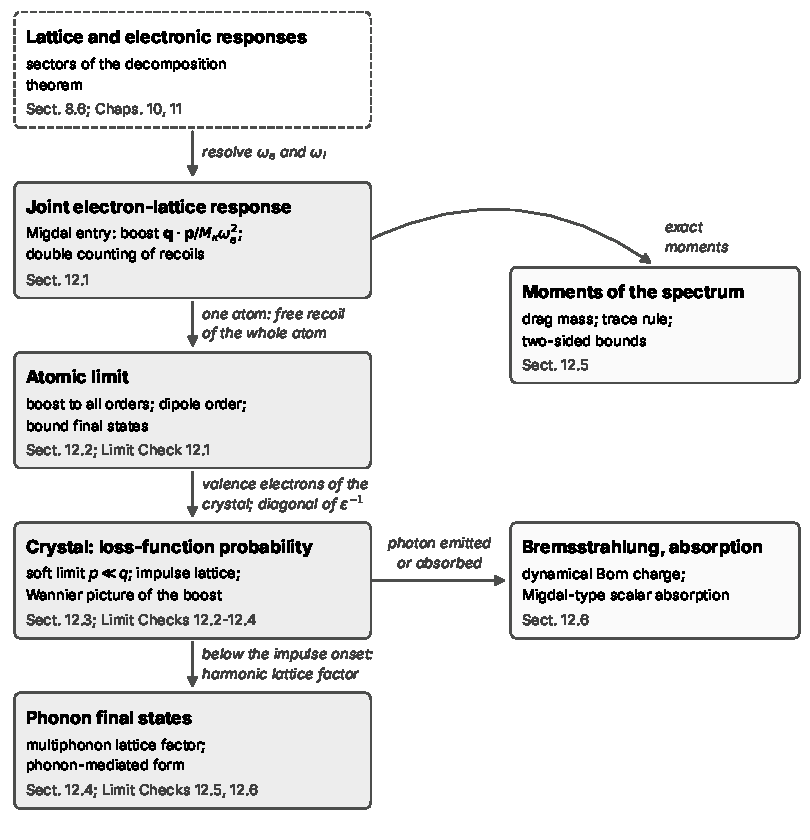
\includegraphics[width=0.85\linewidth]{figures/ch12/map12.pdf}
  \caption{The Migdal entry of the joint electron--lattice response and its truncations. Resolving the energy given to the electrons, $\omega_e$, and to the lattice, $\omega_l$, in the sectors of \cref{sec:8.6} gives the joint response, whose Migdal entry is a boost $\vect{q}\cdot\vect{p}/M_\kappa\omega_e^2$ (\cref{sec:12.1}). One atom with a free recoil gives the atomic limit (\cref{sec:12.2}; \cref{lim:12.2a}); the valence electrons of the crystal with the diagonal of $\varepsilon^{-1}$ give the loss-function probability (\cref{sec:12.3}; \cref{lim:12.3a,lim:12.3b,lim:12.3c}); below the impulse onset the harmonic lattice factor gives the phonon final states (\cref{sec:12.4}; \cref{lim:12.4a,lim:12.4b}). Branches: the exact moments of the spectrum (\cref{sec:12.5}), and the emission or absorption of a photon or scalar (\cref{sec:12.6}).}
  \label{fig:12-map}
\end{figure}

\section{The joint electron--lattice response}\label{sec:12.1}

At a momentum transfer of \SI{50}{keV} a silicon nucleus receives the recoil energy $E_R = q^2/2M_\kappa = \SI{47.8}{meV}$. The lattice takes the recoil energy as a few phonons: the Debye--Waller exponent is $2W_\kappa = 1.57$, and in \SI{21}{\percent} of the kicks the lattice is left as it was (\cref{sec:11.3}). In about three kicks in a million, in the model of \cref{fig:12-plane} below, the electrons do not follow the nucleus, and an electron--hole pair of a few eV is made as well. An event with a pair deposits about \SI{6}{eV}, of which \SI{48.5}{meV} are in the lattice and the rest in the electrons, and a detector treats the two parts differently. The electronic energy makes charge at once; the lattice energy lies below the gap and reaches only a phonon sensor (\cref{chap:18,chap:20}). The response $S_{ab}(\vect{q},\omega)$ of the master formula \cref{eq:8.2-spectrum} cannot separate the electronic energy from the lattice energy, because it adds all final states of the same total energy $\omega$. We need a response with two energy arguments.

\subsection{The joint response}\label{sec:12.1-def}

Every prompt final state $f$ of \cref{sec:8.7-classes} has a definite electronic content: none in the electron-following sector, and otherwise an electron--hole pair, an exciton or a core hole, with or without phonons. We give it an \emph{electronic energy} $E^{\mathrm{el}}_f$, zero in $\mathcal{P}_{\mathrm{ad}}$ and otherwise the zero-phonon energy of its electronic excitation; for a pair this is the quasiparticle energy $\tilde E_m$ of \cref{eq:8.6-dyson}. The remaining energy of the final state, $E_f - E^{\mathrm{el}}_f$, belongs to the lattice: phonons and a recoil. Sorting the final-state-resolved response \cref{eq:8.7-resolved} by the two energies defines the \emph{joint response}
\begin{equation}
  S_{ab}(\vect{q};\omega_l,\omega_e) = \frac{2\pi}{\Vol}\sum_{i,f}p_i\,\langle i|O_a(\vect{q})^\dagger|f\rangle\langle f|O_b(\vect{q})|i\rangle\,
  \delta\bigl(\omega_e - E^{\mathrm{el}}_f + E^{\mathrm{el}}_i\bigr)\,\delta\bigl(\omega_l - (E_f - E^{\mathrm{el}}_f) + (E_i - E^{\mathrm{el}}_i)\bigr) ,
  \label{eq:12.1-joint}
\end{equation}
with $\omega_e$ the energy given to the electrons and $\omega_l$ the energy given to the lattice. At $T \ll \Eg$ every initial state has $E^{\mathrm{el}}_i = 0$. Integrating over $\omega_e$ at fixed total energy removes one delta function and returns the response of \cref{sec:4.2},
\begin{equation}
  \int\dd\omega_e\;S_{ab}(\vect{q};\omega - \omega_e,\omega_e) = S_{ab}(\vect{q},\omega) .
  \label{eq:12.1-marginal}
\end{equation}
The properties of the resolved response carry over to the joint response (\cref{app:D.33}). Where the electronic energy is a good label, each point of the $(\omega_l, \omega_e)$ plane is a sum of outer products with positive weights, and the matrix $S_{ab}(\vect{q};\omega_l,\omega_e)$ is positive semidefinite at every $(\omega_l, \omega_e)$. The rate into a region of the plane is a double spectrum $\dd^2\mathcal{R}/\dd\omega_l\,\dd\omega_e$: \cref{eq:8.2-spectrum} with the joint response \cref{eq:12.1-joint} in place of $S_{ab}(\vect{q},\omega)$ and $\omega = \omega_l + \omega_e$ in the delta function. The cascade of \crefrange{chap:18}{chap:20} turns this double spectrum, not $\dd\mathcal{R}/\dd\omega$, into charge and phonon signals.

The electronic energy is a label, and it is defined where \cref{sec:8.6} defines labels. Inside the off-shell window it is unique to relative order $\theta_{\mathrm{ep}}$. Near a resonant zero-phonon pair the Dyson convention \cref{eq:8.6-dyson} decides: the delta part of \cref{eq:8.6-dyson} lies at $(\omega_l, \omega_e) = (0, \tilde E_m)$, and its finite-part and principal-value parts at the pair energy and $\omega_l = \pm\omega_{\vect{Q}\nu}$ of the phonon made with the pair. We take the zero-phonon energy, and not the vertical energy at the equilibrium positions, because the two differ by the energy the lattice gains when it relaxes around the excitation, and that energy ends up in phonons. For a pair spread over many cells the difference is negligible, since a delocalized pair displaces no nucleus (\cref{sec:8.6}); for a localized excitation it is not, as \cref{we:12-oscillator} shows.

At $T = 0$ the three sectors of \cref{eq:8.6-partition} fall on three parts of the plane,
\begin{equation}
  S_{ab}(\vect{q};\omega_l,\omega_e) = \underbrace{\delta(\omega_e)\,S^{\mathrm{ad}}_{ab}(\vect{q},\omega_l)}_{\text{electron-following}} + \underbrace{\delta(\omega_l)\,S^0_{ab}(\vect{q},\omega_e)}_{\text{zero-phonon electronic}} + \underbrace{S^+_{ab}(\vect{q};\omega_l,\omega_e)}_{\text{phonon-dressed electronic}} ,
  \label{eq:12.1-sectors}
\end{equation}
with $S^{\mathrm{ad}}_{ab}$ and $S^0_{ab}$ the sector responses \cref{eq:8.6-sector}, each a function of one energy. The electron-following sector is the line $\omega_e = 0$, the zero-phonon electronic sector the line $\omega_l = 0$, and the phonon-dressed sector fills the quadrant $\omega_l, \omega_e > 0$. In a warm target phonons can also be absorbed, and $\omega_l$ takes either sign.

Each row of the master formula occupies its own parts of the plane. The electron density has weight in three places. The phonons excited through the electrons that follow the nuclei (\cref{eq:8.6-follow}) lie on the line $\omega_e = 0$, the clamped-nuclei response of \cref{chap:10} lies on the line $\omega_l = 0$, and the phonon sideband of \cref{chap:13} lies at $\omega_l = \pm\omega_{\vect{Q}\nu}$ for one phonon. The nuclear density puts the lattice response of \cref{chap:11}, single phonons, multiphonons and free recoil, on the line $\omega_e = 0$. The weight of the nuclear density off that line is the Migdal effect, which the rest of this chapter computes. The interference $S_{e\kappa}$ of the two densities is the Born-charge interference of \cref{sec:8.4} on the line $\omega_e = 0$. Off that line it is the interference of a Migdal amplitude with an electron-recoil amplitude into the same final state, a zero-phonon pair at $\omega_l = 0$ or a pair with a phonon at $\omega_l = \omega_{\vect{Q}\nu}$. Positivity bounds $S_{e\kappa}$ at every point of the plane, $|S_{e\kappa}|^2 \le S_{ee}S_{\kappa\kappa}$ (\cref{eq:4.2-positivity}), and \cref{sec:12.5,sec:17.4} compute it.

\subsection{The boosted electronic response}\label{sec:12.1-boost}

The nuclear density reaches the electronic sectors only through the nonadiabatic coupling. \Cref{eq:8.6-boost} gives the amplitude at first order in the nonadiabatic coupling: a kick $\ee^{\ii\vect{q}\cdot\vect{X}_I}$ excites the electrons to $\Psi_j$ with the factor $-\ii\,\vect{q}\cdot\vect{d}^I_{j0}/(M_\kappa\Delta E_j)$, times the kick of the nuclear wavefunction. To turn this amplitude into a response we write the derivative coupling as the matrix element of an operator whose response we know. By \cref{eq:5.1-dcoup}, $\vect{d}^I_{j0} = -\vect{F}^I_{j0}/\Delta E_j$, with $\vect{F}^I_{j0}$ the matrix element of the force that nucleus $I$ exerts on the electrons. Let the nucleus act on the electrons through a potential $v_\kappa$ that moves rigidly with it, the bare Coulomb potential $-Z_\kappa e^2/(4\pi r)$ or a pseudopotential (\cref{sec:6.1}). With the Fourier convention \cref{eq:A.3-space}, the projected force is a sum of density components,
\begin{equation}
  \vect{q}\cdot\nabla_{\vect{X}_I}V_{eN} = -\ii\int\frac{\dd^3p}{(2\pi)^3}\;(\vect{q}\cdot\vect{p})\,v_\kappa(\vect{p})\,\ee^{-\ii\vect{p}\cdot\vect{X}_I}\,n_e(\vect{p}) .
  \label{eq:12.1-force}
\end{equation}
The nucleus is, for its electrons, an external potential with Fourier components $v_\kappa(\vect{p})$, and moving it by $\delta\vect{X}$ changes each component by $-\ii\vect{p}\cdot\delta\vect{X}$ times itself. Here $\vect{p}$ is the momentum given to the electrons. Inserting \cref{eq:12.1-force} in \cref{eq:8.6-boost} gives (\cref{app:D.33-amp})
\begin{equation}
  \bigl\langle\Psi^{\mathrm{nuc}\prime}\Psi_j\big|n_\kappa(\vect{q})\big|\Psi^{\mathrm{nuc}}\Psi_0\bigr\rangle
  = \sum_{I\in\kappa}\int\frac{\dd^3p}{(2\pi)^3}\;\frac{\vect{q}\cdot\vect{p}}{M_\kappa\Delta E_j^2}\,v_\kappa(\vect{p})\,\langle\Psi_j|n_e(\vect{p})|\Psi_0\rangle\,\bigl\langle\Psi^{\mathrm{nuc}\prime}\big|\ee^{\ii(\vect{q} - \vect{p})\cdot\vect{X}_I}\big|\Psi^{\mathrm{nuc}}\bigr\rangle .
  \label{eq:12.1-amp}
\end{equation}
Read from right to left, \cref{eq:12.1-amp} says that the nucleus takes the kick $\vect{q}$, passes the momentum $\vect{p}$ to the electrons through its own field and keeps $\vect{q} - \vect{p}$; the electrons are excited by the density component $n_e(\vect{p})$, as by any external potential. The factor $\vect{q}\cdot\vect{p}/(M_\kappa\Delta E_j) = \vect{v}_N\cdot\vect{p}/\Delta E_j$ is the sudden amplitude \cref{eq:6.1-sudden1}, and the remaining $v_\kappa/\Delta E_j$ turns the force into a derivative coupling.

\Cref{eq:12.1-amp} takes the transition density $\langle\Psi_j|n_e(\vect{p})|\Psi_0\rangle$ at the equilibrium positions (the Condon approximation of \cref{sec:5.6}) and takes the vibrational final states on the ground surface, so that $\Delta E_j$ is the vertical excitation energy; for a delocalized pair it is also the zero-phonon energy. Freezing the transition density in the frame of the crystal makes the lattice recoil with $\vect{q} - \vect{p}$, as in the crystal formulas of Knapen, Kozaczuk and Lin~\cite[Eq.~(3)]{knapen2021migdal} and of Berghaus and collaborators~\cite[Eq.~(3.8)]{berghaus2023migdal}. For an isolated atom, whose electrons move with the nucleus, the same steps give $\ee^{\ii\vect{q}\cdot\vect{X}}$: the whole atom recoils (\cref{app:D.33-amp}). Valence electrons in a crystal lie between these two cases, the frame of the crystal and the frame of the struck ion, and it is an open question which of the two frames their transition densities follow. The difference between the two frames is a Herzberg--Teller term, which is the dependence of the transition density on the displacement in \cref{eq:8.6-electronic}. The Herzberg--Teller term changes the momentum the lattice keeps and leaves the electronic spectrum unchanged: at $q = \SI{5}{keV}$ it changes the fraction of Migdal events that emit phonons by a factor 2.4 (\cref{sec:12.4}).

Squaring \cref{eq:12.1-amp}, summing over nuclei and final states, and using the conservation of crystal momentum by the electronic transition (\cref{app:D.33-square}), we obtain the entry of the joint response that holds the Migdal effect.
\begin{keyresult}[The Migdal entry of the joint response]
At Born--Oppenheimer order $n_B = 2$, with Condon transition densities and lattice final states on the ground surface, the nuclear density of species $\kappa$ has, for $\omega_e > 0$,
\begin{equation}
  \begin{split}
  S_{\kappa\kappa}(\vect{q};\omega_l,\omega_e) = \frac{1}{2\pi}\int_{\mathrm{BZ}}\frac{\dd^3k}{(2\pi)^3}\sum_{\vect{G}\vect{G}'}\;
  &\underbrace{\frac{[\vect{q}\cdot(\vect{k}+\vect{G})]\,[\vect{q}\cdot(\vect{k}+\vect{G}')]}{M_\kappa^2\,\omega_e^4}}_{\text{boost}}\;
  \underbrace{v_\kappa(\vect{k}+\vect{G})^*\,v_\kappa(\vect{k}+\vect{G}')}_{\text{vertex}} \\
  &\times\underbrace{S^{ee}_{\vect{G}\vect{G}'}(\vect{k},\omega_e)}_{\text{electrons}}\;
  \underbrace{S^{\mathrm{ad}}_{\kappa;\vect{G}\vect{G}'}(\vect{q} - \vect{k},\omega_l)}_{\text{lattice}} ,
  \end{split}
  \label{eq:12.1-Skk}
\end{equation}
where $S^{ee}_{\vect{G}\vect{G}'}(\vect{k},\omega) = (2\pi/\Vol)\sum_{j\neq0}\langle\Psi_0|n_e(\vect{k}+\vect{G})^\dagger|\Psi_j\rangle\langle\Psi_j|n_e(\vect{k}+\vect{G}')|\Psi_0\rangle\,\delta(\omega - \Delta E_j)$ is the density response matrix of the electrons at clamped nuclei and $S^{\mathrm{ad}}_{\kappa;\vect{G}\vect{G}'}(\vect{Q},\omega)$ the electron-following response \cref{eq:8.6-sector} between $n_\kappa(\vect{Q} - \vect{G})$ and $n_\kappa(\vect{Q} - \vect{G}')$. The zero-phonon part of the Migdal entry, at $\omega_l = 0$, lies in $\mathcal{P}_0$, and the rest in $\mathcal{P}_+$.
\end{keyresult}
\noindent The electronic factor is the full response of the interacting electrons, with screening and local fields inside it, and the vertex is the bare potential of the nucleus. The moving nucleus is an external charge to the electrons, exactly as the dark matter is in the loss-function rate of \cref{sec:10.2}. If the core electrons are frozen into a pseudopotential, $v_\kappa$ is that pseudopotential and $S^{ee}$ the response of the valence electrons; \cref{sec:12.3} works in this frozen-core setting. The lattice factor is the response of \cref{chap:11}, evaluated at the momentum $\vect{q} - \vect{k} - \vect{G}$ that the nucleus keeps.

The size of the effect follows from the moments of $S^{ee}$. The first electronic moment of the Migdal probability is fixed by the drag mass, $\int\dd\omega_e\,\omega_e\,\dd P_{\mathrm{Mig}}/\dd\omega_e = E_R\,\delta M_\kappa/M_\kappa$ for an isotropic drag mass (\cref{eq:8.6-fsum-k}). With a typical electronic energy $\langle\omega_e\rangle$, therefore,
\begin{equation*}
  P_{\mathrm{Mig}} \approx \frac{E_R}{\langle\omega_e\rangle}\,\frac{\delta M_\kappa}{M_\kappa} ,
\end{equation*}
the recoil energy in units of the typical electronic energy, times the share of the mass that the electrons carry. For silicon at $q = \SI{50}{keV}$, with the atomic estimate $\delta M_\kappa/M_\kappa = 2.7\times10^{-4}$ of \cref{sec:8.6} and $\langle\omega_e\rangle \approx \SI{6}{eV}$, $P_{\mathrm{Mig}}$ is about $2\times10^{-6}$. The atomic estimate of $\delta M_\kappa$ is the sum of the drag masses over all nuclei, while a kick probes only the drag-mass element of the struck nucleus, and in silicon that element is about twice the atomic value (\cref{sec:12.5-trace}). The agreement with the model below is therefore partly fortuitous. Since $E_R$ grows as $q^2$, so does $P_{\mathrm{Mig}}$, and the Migdal effect matters where the recoil itself is invisible: it trades the factor $P_{\mathrm{Mig}}$ for an energy $\langle\omega_e\rangle/E_R$ times larger, 120 times at \SI{50}{keV} in silicon.

\Cref{fig:12-plane} shows the plane for silicon at $q = \SI{50}{keV}$, in a model that keeps the valence electrons, the diagonal $\vect{G} = \vect{G}'$ and the incoherent lattice factor, \cref{eq:12.4-harm}. The line $\omega_e = 0$ carries the lattice spectrum of \cref{sec:11.3}, with the zero-phonon weight $\ee^{-2W_\kappa} = 0.21$ and the mean $E_R$. The Migdal weight, $P_{\mathrm{Mig}} = 2.92\times10^{-6}$, or $6.1\times10^{-5}$ per eV of recoil energy (\cref{sec:12.3}), lies at $\omega_e$ above the gap: half of it below \SI{4.4}{eV}, \SI{89}{\percent} below \SI{10}{eV}, with a mean of \SI{5.9}{eV}. Along $\omega_l$ the Migdal weight repeats the lattice spectrum. The line $\omega_l = 0$ holds \SI{21}{\percent} of the Migdal weight, and the rest has the peaks of the phonon density of states. The mean lattice energy of a Migdal event is \SI{48.5}{meV}, above $E_R$ by $\langle p^2\rangle/2M_\kappa$, the recoil of the momentum the electrons take, with $\langle p^2\rangle^{1/2} = \SI{6.1}{keV}$. The map is close to a product of the lattice spectrum and the electronic spectrum. That product is the soft limit $p \ll q$, which \cref{sec:12.3} makes precise; here $p/q$ is about 0.1.

\begin{figure}[tbp]
  \centering
  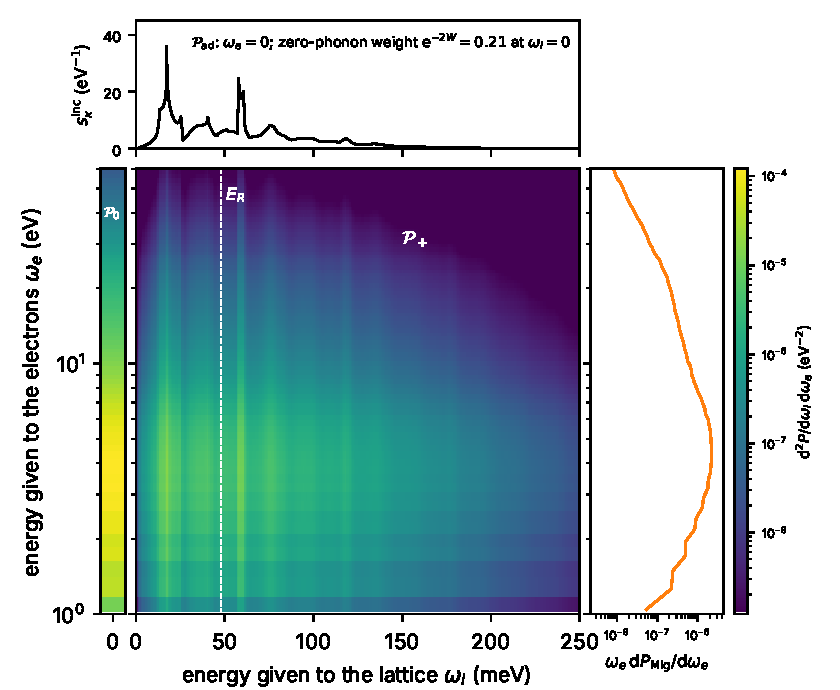
\includegraphics[width=0.92\linewidth]{figures/ch12/fig12_1.pdf}
  \caption{The joint response of silicon at $q = \SI{50}{keV}$ in the plane of the energy $\omega_l$ given to the lattice and the energy $\omega_e$ given to the electrons, per nucleus and normalized as probabilities, at $T = 0$. Top: the electron-following line $\omega_e = 0$, the incoherent lattice spectrum $s^{\mathrm{inc}}_\kappa$ of one nucleus without its zero-phonon part $\ee^{-2W} = 0.21$ at $\omega_l = 0$ ($E_R = \SI{47.8}{meV}$, $2W = 1.57$, phonon density of states from density-functional perturbation theory). Main panel: the Migdal probability density $\dd^2P/\dd\omega_l\,\dd\omega_e$ in the phonon-dressed sector $\mathcal{P}_+$; the dashed line marks $E_R$. Left strip: the zero-phonon Migdal line $\omega_l = 0$ (sector $\mathcal{P}_0$), drawn as a bin of \SI{1}{meV} in $\omega_l$ on the same color scale. Right: the marginal $\omega_e\,\dd P_{\mathrm{Mig}}/\dd\omega_e$. Model: \cref{eq:12.1-Skk} with valence electrons only, the ion charge $Z_{\mathrm{ion}}(p)$ of \cref{eq:12.3-Zion} and the diagonal $\vect{G} = \vect{G}'$. The electronic factor is the random-phase loss function of silicon with local fields of Knapen, Kozaczuk and Lin~\cite{knapen2021dark} (threshold \SI{1.11}{eV}, the step-model gap that accompanies the tables, $p \le \SI{22.5}{keV}$, $\omega_e \le \SI{89}{eV}$, averaged over directions); the transition densities are Condon in the frame of the crystal (lattice factor at $|\vect{q} - \vect{p}|$), and the lattice response is incoherent.}
  \label{fig:12-plane}
\end{figure}

The energy denominators of the boost neglect the nuclear motion against $\omega_e$, at relative order $v_Np/\omega_e$ and $(\omega_l/\omega_e)^2$; at the momenta of \cref{fig:12-plane} these are $3\times10^{-3}$ and $10^{-4}$. The exact denominators are \cref{eq:12.3-bracket} for a free nucleus and \cref{eq:12.4-exact} for a bound one. The Condon approximation drops the change of the transition density with the displacements, the Herzberg--Teller term above. The ground-surface final states drop the displacement of the excited surface, which moves energy from $\omega_e$ to $\omega_l$ without changing their sum, and which is negligible for a delocalized pair. \Cref{we:12-oscillator} shows the Herzberg--Teller term and the excited-surface displacement at work where they are not small.

\Cref{app:E.6} gives the dielectric matrix of the electrons, with local fields, on a grid of $(\vect{k}, \omega_e)$, and \cref{app:E.17} gives the lattice response on a grid of momenta.

\begin{workedexample}{The joint response of a displaced oscillator}\label{we:12-oscillator}
We take the model, the kick $\ee^{\ii qx}$ with $q\ell_0 = 1$ ($E_R = \omega_0 = \SI{64.1}{meV}$) and the labels of \cref{we:8-sectors}. A state on the excited surface with vibrational level $m$ gets $\omega_e = \SI{1.0463}{eV}$, the zero-phonon energy of the upper level, and $\omega_l = m \times \SI{65.5}{meV}$, the quanta of the excited surface, both read off the exact diagonalization.

\emph{The exact plane.} The line $\omega_e = 0$ carries the kick on the ground surface, with weight $1 - P_{\mathrm{Mig}}$. The Migdal weight $P_{\mathrm{Mig}} = 3.94\times10^{-6}$ of \cref{we:8-sectors} lies on the line $\omega_e = \SI{1.0463}{eV}$ as a comb in $\omega_l$, with the fractions 0.097, 0.227, 0.265, 0.205, 0.119 and 0.055 for $m = 0$ to 5. The lattice receives on average \SI{0.153}{eV} in a Migdal event, more than twice the recoil energy.

\emph{The leading entry with ground-surface final states.} This entry is \cref{eq:12.1-Skk}: every Migdal event sits at the vertical energy $\omega_e = \Delta_{\mathrm{tl}} = \SI{1.17}{eV}$, and the lattice factor is the kick of the ground surface, Poisson distributed with mean $(q\ell_0)^2 = 1$. The fractions are 0.368, 0.368, 0.184, 0.061, and the mean lattice energy is $E_R = \SI{64.1}{meV}$. The total energy per event, $\Delta_{\mathrm{tl}} + E_R = \SI{1.234}{eV}$, is close to the exact \SI{1.199}{eV}, but the split between electrons and lattice is wrong.

\emph{Excited-surface final states.} Projecting the kicked state on the vibrational states of the excited surface puts the relaxation energy in $\omega_l$. For surfaces of equal frequency the overlap $\langle m_{\mathrm{up}}|\ee^{\ii qx}|0_{\mathrm{lo}}\rangle$ is that of a coherent state whose amplitude adds the imaginary kick $\ii q\ell_0$ to the real displacement $-S_{\mathrm{HR}}^{1/2}$. The weights are then Poisson with mean $(q\ell_0)^2 + S_{\mathrm{HR}} = 3$, and the mean lattice energy is $3\omega_0 = \SI{0.192}{eV}$, against $E_R$ before. On the computed surfaces, with their unequal quanta, the same projection gives the mean lattice energy \SI{0.188}{eV} and the zero-phonon fraction 0.056 instead of $\ee^{-3} = 0.050$, with the derivative coupling evaluated at $x = 0$ (the Condon approximation). The relaxation energy $S_{\mathrm{HR}}\omega_0 = \SI{0.128}{eV}$ has moved from $\omega_e$ to $\omega_l$, and the total $\SI{1.0463}{eV} + \SI{0.188}{eV} = \SI{1.234}{eV}$ is unchanged. The probability is $3.52\times10^{-6}$, the value of the boost formula of \cref{we:8-sectors}, and the zero-phonon fraction 0.056 falls short of the exact 0.097.

\emph{Beyond Condon.} The derivative coupling and the gap both vary along $x$: the gap is $\Delta_{\mathrm{tl}} + g_{\mathrm{d}}x/\ell_0$, smaller on the side of the displaced minimum. Keeping $q\,d_{10}(x)/[(M/2)\Delta E(x)]$ inside the vibrational matrix element, as a function of $x$, gives $P_{\mathrm{Mig}} = 4.00\times10^{-6}$, the fractions 0.104, 0.236, 0.267, 0.201, 0.113 and 0.051, and the mean lattice energy \SI{0.148}{eV}, all within a few percent of the exact values. \Cref{we:8-sectors} traced the \SI{12}{\percent} excess of the exact probability over the boost formula to the displaced surface; this excess is the Herzberg--Teller term, and it acts most on the zero-phonon line.

A strongly displaced excited surface, as for an exciton bound to a defect, therefore needs the zero-phonon energy as its electronic energy and the non-Condon term. For an electron--hole pair spread over $N$ cells, $S_{\mathrm{HR}}$ is of order $1/N$, and the ground-surface form \cref{eq:12.1-Skk} is the right one.
\end{workedexample}

\subsection{Local fields and the choice of electrons}\label{sec:12.1-truncations}

Each truncation of \cref{fig:12-map} keeps the boost and makes a choice for the vertex, the electronic factor and the lattice factor. On the diagonal of $\varepsilon^{-1}$ the local fields lower the silicon probability by a factor 1.35 against a scalar dielectric function (\cref{lim:12.3a}). Through the off-diagonal elements $\vect{G} \neq \vect{G}'$ they couple different momenta. No table in this book contains the off-diagonal part; it is sized only in a model of silicon, where it raises the rate, and the full calculation is still open (\cref{sec:12.3-validity}). The same matrix $\varepsilon^{-1}$ changes the electron-recoil rate of silicon by a factor of 1.5 at \SI{10}{MeV} (\cref{sec:10.2-corrections}). The atomic formula, applied to the valence electrons of a crystal, puts the wrong electrons in the electronic factor. The valence electrons of silicon are not those of a silicon atom, and their gap is \SI{1.17}{eV} instead of the atomic binding of several eV; the factor $\omega_e^{-4}$ magnifies the difference between the two energies. For the core shells, whose electrons do move with their nucleus, the atomic form is the right truncation (\cref{sec:12.2}).

\subsection{Double counting of recoils}\label{sec:12.1-counting}

The joint response holds the lattice and the Migdal parts of one nuclear response, and its moments fix how they add. Take the incoherent response, one nucleus at a time. The total weight of $n_\kappa(\vect{q})$ is $2\pi\nd_\kappa$, the density of nuclei times $2\pi$, whatever the final states; integrated over the plane, \cref{eq:12.1-joint} has that weight. The Migdal entry takes $2\pi\nd_\kappa P_{\mathrm{Mig}}(q)$ of it, and the line $\omega_e = 0$ keeps
\begin{equation}
  \int\dd\omega_l\;S^{\mathrm{ad}}_{\kappa\kappa}(\vect{q},\omega_l) = 2\pi\nd_\kappa\bigl[1 - P_{\mathrm{Mig}}(q)\bigr] .
  \label{eq:12.1-zeroth}
\end{equation}
The first moment of the line, by \cref{eq:8.6-fsum-k}, is that of a nucleus of mass $M_\kappa + \delta M_\kappa$. The lattice responses of \cref{chap:11} are normalized to unit weight and use the bare mass. Added to a Migdal rate, they count twice the kicks that excited the electrons: once as pure recoils on the line $\omega_e = 0$ and once as Migdal events. The double count is a fraction $P_{\mathrm{Mig}}$ of the kicks, but in each of them the lattice energy is not small: \cref{fig:12-plane} shows that a Migdal event carries the whole recoil, \SI{48.5}{meV} on average against $E_R = \SI{47.8}{meV}$, and the electronic energy on top of it. The consistent sum takes the lattice response with the weight $1 - P_{\mathrm{Mig}}$ and the mass $M_\kappa + \delta M_\kappa$, the first prescription of \cref{sec:8.6}, and the joint response applies this prescription by construction. In silicon the weight correction $P_{\mathrm{Mig}}$ and the mass correction $\delta M_\kappa/M_\kappa$ are both below $10^{-3}$ for $E_R \lesssim \SI{16}{eV}$, which covers the phonon and multiphonon momenta of \cref{chap:11}, and the rate of a phonon detector does not see the two corrections there. At \SI{500}{eV} the weight $1 - P_{\mathrm{Mig}}$ is a \SI{3}{\percent} correction (\cref{sec:12.5-bounds}). The counting of Migdal and lattice events, however, is exact, and \cref{sec:12.5} completes it with the higher moments.

The same entry fixes the lattice factor of the Migdal rate itself. A Migdal event leaves the lattice in the state that the kick $\vect{q} - \vect{p}$ makes, so the lattice factor of a Migdal rate below the impulse onset is the multiphonon response of \cref{sec:11.3}, not a free recoil. Combining a free-recoil Migdal formula with a multiphonon lattice rate counts nothing twice; it mixes two truncations of one response, and a rate built that way is labeled by neither. On the scale of \cref{sec:8.5} the two pieces of a rate should carry the same lattice regime $\mathcal{K}$.

Measured nuclear-recoil signals obey the same rule from the other side. A calibration with neutrons measures the ionization of nuclear recoils, and the Migdal electrons of those recoils are part of what it measures. A nuclear-recoil rate converted to charge with a measured yield already contains the Migdal ionization, and a computed Migdal rate added to it counts that ionization twice. The yield and its Migdal part are separated in \cref{sec:19.2}.

\subsection{Targets without a gap}\label{sec:12.1-gapless}

The construction used the gap three times: to give each final state an electronic energy, to make the energy denominators of the boost large compared with the lattice energies, and to keep the low-energy end of $S^{ee}$ empty. In a metal, a superconductor or a semimetal all three fail.

With the quasiparticle sectors $\mathcal{P}^{\mathrm{qp}}_{n,m}$ of \cref{sec:8.6}, $\omega_e$ becomes the energy of the quasiparticles created, defined to within their width, and the joint response is meaningful on bins of the plane that satisfy the bin bound \cref{eq:8.6-bin}.

In a metal the loss function grows linearly from $\omega_e = 0$, since electron--hole pairs at the Fermi surface cost nothing, and with the factor $\omega_e^{-4}$ the Migdal probability \cref{eq:12.1-Skk} integrates as $\int\dd\omega_e\,\omega_e^{-3}$ and diverges at small $\omega_e$. The divergence marks the failure of the sudden expansion, not a large effect. Once $\omega_e$ falls to the phonon energies, the electrons follow the nucleus instead of being left behind. The boost denominator $\omega_e^2$ must then be replaced by the full denominator. For a bound nucleus the full denominator is the phonon propagator $\omega_e^2 - \omega_{\mathrm{ph}}^2$ of the phonon-mediated form, whose pole at $\omega_e = \omega_{\mathrm{ph}}$ is the ordinary electron--phonon coupling of \cref{chap:6}. The part of the plane with $\omega_e \lesssim \omega_{\mathrm{D}}$ then belongs to the electron--phonon response of the metal, computed with Fan--Migdal and Eliashberg methods (\cref{sec:6.3,sec:6.4}), and only $\omega_e \gg \omega_{\mathrm{D}}$ is a Migdal process in the sense of this chapter. The electronic factor also changes character: $S^{ee}$ contains the intraband response of the conduction electrons, which screens the moving ion at small $\omega_e$, so that a slowly moving ion in a metal carries no charge. The full response contains this intraband screening, and a formula that screens the vertex statically does not. In a superconductor, whose hierarchy is reversed (\cref{sec:8.6}), a kicked nucleus breaks pairs through the phonons it emits (\cref{chap:15,chap:20}).

\section{The atomic limit}\label{sec:12.2}

A germanium atom that recoils with \SI{1}{keV} loses an electron to the continuum in one recoil in 580 according to the calculation of Ibe and collaborators, and in one recoil in 610 according to that of Cox and collaborators; in one recoil in 230 its electrons are left excited or ionized. Most of these events come from two shells, the $3d$ shell, bound by about \SI{30}{eV} and smaller than an angstrom, and the valence shell. A crystal of germanium keeps the first nearly as it is in the atom and rebuilds the second into bands. In the atom the Migdal entry \cref{eq:12.1-Skk} of the joint response can be evaluated to all orders in the momentum given to the electrons, and every number can be checked against a sum rule.

\subsection{The boost of a free atom}\label{sec:12.2-boost}

Take one atom at rest in its ground state, with a nucleus of mass $M$ at $\vect{X}$ and $N_e$ electrons at $\vect{r}_e$. Dark matter couples to the nucleus through $\ee^{\ii\vect{q}\cdot\vect{X}}$, to first order in the coupling. The Coulomb energy depends only on the positions of the electrons relative to the nucleus, $\vect{\rho}_e = \vect{r}_e - \vect{X}$. We trade $\vect{X}$ for the center of mass $\vect{R}_{\mathrm{cm}} = (M\vect{X} + m_e\sum_e\vect{r}_e)/m_A$ and keep the $\vect{\rho}_e$, with
\begin{equation}
  m_A = M + N_em_e ,
  \label{eq:12.2-mA}
\end{equation}
the mass of the atom up to the binding energy of its electrons, less than a part in $10^{6}$. The chain rule gives $\nabla_{\vect{X}} = (M/m_A)\nabla_{\vect{R}_{\mathrm{cm}}} - \sum_e\nabla_{\vect{\rho}_e}$ and $\nabla_{\vect{r}_e} = (m_e/m_A)\nabla_{\vect{R}_{\mathrm{cm}}} + \nabla_{\vect{\rho}_e}$. In the kinetic energy $-\nabla_{\vect{X}}^2/2M - \sum_e\nabla_{\vect{r}_e}^2/2m_e$ the cross terms between $\nabla_{\vect{R}_{\mathrm{cm}}}$ and $\nabla_{\vect{\rho}_e}$ cancel, and the terms in $\nabla_{\vect{R}_{\mathrm{cm}}}^2$ add up to $1/2m_A$. The Hamiltonian separates exactly,
\begin{equation}
  H = -\frac{\nabla_{\vect{R}_{\mathrm{cm}}}^2}{2m_A} + H_{\mathrm{rel}} , \qquad
  H_{\mathrm{rel}} = -\sum_e\frac{\nabla_{\vect{\rho}_e}^2}{2m_e} - \frac{1}{2M}\Bigl(\sum_e\nabla_{\vect{\rho}_e}\Bigr)^2 + V_{eN} + V_{ee} .
  \label{eq:12.2-Hint}
\end{equation}
The internal Hamiltonian is the clamped-nucleus Hamiltonian of \cref{sec:5.1} plus one term, the kinetic energy $(\sum_e\vect{p}_e)^2/2M$ of a nucleus that balances the momentum of its electrons. Its diagonal part turns $m_e$ into the reduced mass, and its off-diagonal part, $-M^{-1}\sum_{e<e'}\nabla_{\vect{\rho}_e}\cdot\nabla_{\vect{\rho}_{e'}}$, is the mass-polarization term of atomic physics. Both change energies and wavefunctions at relative order $m_e/M$.

The kick separates just as exactly. Since $\vect{X} = \vect{R}_{\mathrm{cm}} - (m_e/m_A)\sum_e\vect{\rho}_e$,
\begin{equation}
  \ee^{\ii\vect{q}\cdot\vect{X}} = \ee^{\ii\vect{q}\cdot\vect{R}_{\mathrm{cm}}}\;\exp\Bigl(-\ii\vect{q}_e\cdot\sum_e\vect{\rho}_e\Bigr) , \qquad
  \vect{q}_e = \frac{m_e}{m_A}\,\vect{q} = m_e\vect{v}_A ,
  \label{eq:12.2-cm}
\end{equation}
with $\vect{v}_A = \vect{q}/m_A$ the velocity of the recoiling atom. The first factor gives the whole atom the momentum $\vect{q}$ and the kinetic energy $q^2/2m_A$. The second acts on the internal state alone, as a momentum $-\vect{q}_e$ given to every electron. For hydrogen this is the separation of \cref{sec:6.1}. With $N_e$ electrons the center of mass still separates exactly; what the other electrons change is the internal Hamiltonian, through the mass-polarization term, and the boost mass, $m_A$ in place of the proton mass. The joint response \cref{eq:12.1-joint} of a gas of $\nd_T$ such atoms per unit volume, incoherent between atoms, is therefore
\begin{keyresult}[Migdal effect of a free atom]
\begin{gather}
  S_{\kappa\kappa}(\vect{q};\omega_l,\omega_e) = 2\pi\nd_T\,\delta\Bigl(\omega_l - \frac{q^2}{2m_A}\Bigr)\sum_fP_f(\vect{q})\,\delta(\omega_e - E_f + E_0) , \nonumber\\
  P_f(\vect{q}) = \Bigl|\Bigl\langle\Psi_f\Big|\exp\Bigl(-\ii\vect{q}_e\cdot\sum_e\vect{\rho}_e\Bigr)\Big|\Psi_0\Bigr\rangle\Bigr|^2 ,
  \label{eq:12.2-joint}
\end{gather}
with $\Psi_f$ and $E_f$ the eigenstates and energies of $H_{\mathrm{rel}}$ and $\vect{q}_e = m_e\vect{q}/m_A$. It holds to first order in the dark-matter coupling and to all orders in $q$, with no assumption about time.
\end{keyresult}
\noindent The term $f = 0$ is the line $\omega_e = 0$, the electron-following sector of \cref{eq:12.1-sectors}, with weight $P_0 = 1 - P_{\mathrm{Mig}}$. The rest is the Migdal entry. All of it sits on the line $\omega_l = q^2/2m_A$: a free atom has no phonons, and the lattice energy of every event is the recoil of the atom. \Cref{eq:12.2-joint} is the electron-cloud transition factor of Ibe and collaborators, who derive it in the same way and write the argument as the final velocity of the atom times $m_e$~\cite[Eqs.~(55), (57) and (73)]{ibe2018migdal}. Their phase $\ee^{-\ii\vect{q}_e\cdot\vect{x}}$ in the electron coordinates and the opposite sign of Kahlhoefer and Su~\cite[Eq.~(1)]{kahlhoefer2026probing} leave $|\cdot|^2$ unchanged.

\Cref{sec:6.1} reached the same structure from the other side, as the sudden boost \cref{eq:6.1-boost} with the velocity $v_N = q/M$ of the bare nucleus, and the leading entry \cref{eq:12.1-Skk} carries the same mass. Both are right to the order they claim. The exact separation fixes the next order: the boost mass is $m_A$, and at fixed $q$ the electrons receive $m_eq/m_A$, smaller than $m_eq/M$ by the factor $1 - N_em_e/m_A$. The electrons that follow the nucleus add their mass to it. This is the drag mass of \cref{eq:8.6-fsum-k}, $\delta M = N_em_e$ for an atom, and $M + \delta M = m_A$. The probability changes by $2N_em_e/m_A$, $5.5\times10^{-4}$ for silicon and $4.8\times10^{-4}$ for germanium, far below any other uncertainty of the calculation, but the counting of Migdal and lattice events in \cref{sec:12.5} needs it, and in a crystal the same role falls to $M_\kappa + \delta M_\kappa$ with the tensor drag mass of \cref{sec:8.6}. What the separation leaves to be solved is the internal problem. The states $\Psi_f$ are those of $H_{\mathrm{rel}}$, and the atomic calculations used below solve the clamped-nucleus problem instead, an error of relative order $m_e/M$ in each $P_f$.

The rate of a free-atom target follows from \cref{eq:8.2-spectrum} with the joint response \cref{eq:12.1-joint}. For a spin-independent coupling the nuclear vertex is $AF_N(q)$, the delta function of $\omega_l$ fixes $q = (2m_AE_R)^{1/2}$, and energy conservation needs $\omega_{\vect{q}} = E_R + \omega_e$. With the minimum velocity \cref{eq:1.3-vmin} at $\omega = E_R + \omega_e$, the free-recoil rate \cref{eq:11.4-LS} becomes
\begin{equation}
  \frac{\dd^2\mathcal{R}}{\dd E_R\,\dd\omega_e} = \frac{\rho_\chi\,\sigma_N}{2\mchi\,\mu_{\chi N}^2}\,F_N(q)^2\,\eta\Bigl(\frac{q}{2\mu_{\chi N}} + \frac{\omega_e}{q}\Bigr)\,\frac{\dd P}{\dd\omega_e}(q) ,
  \label{eq:12.2-rate}
\end{equation}
a rate per target atom, with $\mu_{\chi N}$ the reduced mass of the dark matter and the atom and $\dd P/\dd\omega_e = \sum_{f\neq0}P_f\,\delta(\omega_e - E_f + E_0)$. This is the rate of Ibe and collaborators~\cite[Eqs.~(91) and (92)]{ibe2018migdal}. The electronic energy raises $\vmin$ by $\omega_e/q$, and at fixed $\omega_e$ the recoil energy can no longer be arbitrarily small, since $\vmin$ grows without bound as $q \to 0$. The total deposit is at most the kinetic energy $\frac12\mchi v_{\mathrm{max}}^2$ of the dark matter, with the largest laboratory speed $v_{\mathrm{max}} = \SI{795}{km.s^{-1}}$ of the halo of \cref{sec:1.2}, \SI{35}{eV} at \SI{10}{MeV} and \SI{3.5}{keV} at \SI{1}{GeV}, and this, more than the probability, decides which shells a light particle can ionize.

\subsection{Shell probabilities at dipole order}\label{sec:12.2-dipole}

The electrons of an atom receive little momentum. A recoil energy $E_R$ gives them $q_e = m_e(2E_R/m_A)^{1/2}$, \SI{88}{eV} for germanium at $E_R = \SI{1}{keV}$, and the multipole parameter of \cref{sec:8.5} is $\xi_D = q_er_{\mathrm{orb}} = 0.07$ for its valence shell, of mean radius $2.9\,a_0$, and 0.02 for the $3d$ shell. The boost can be expanded. With $D_{\hat q} = \hat{\vect{q}}\cdot\sum_e\vect{\rho}_e$ the dipole operator of the electrons along the kick, the amplitude of an excited state is $-\ii q_e\langle\Psi_f|D_{\hat q}|\Psi_0\rangle$ plus terms of order $q_e^2$, and
\begin{equation}
  P_f = q_e^2\,\bigl|\langle\Psi_f|D_{\hat q}|\Psi_0\rangle\bigr|^2 , \qquad f \neq 0 ,
  \label{eq:12.2-dipole}
\end{equation}
at multipole order $n_D = 2$. Its corrections, of relative order $\xi_D^2$, come from the quadrupole and monopole terms of the boost and from the dipole term at second order. For hydrogen \cref{eq:12.2-dipole} sums to $q_e^2\langle z^2\rangle = q_e^2a_0^2$, the small-$v_N$ form of \cref{eq:6.1-P0}.

Two sums over final states are fixed without solving for any of them. Closure over $f \neq 0$ gives the total probability, and the double commutator of $D_{\hat q}$ with $H_{\mathrm{rel}}$ gives its first moment,
\begin{equation}
  P_{\mathrm{Mig}} = q_e^2\bigl(\langle D_{\hat q}^2\rangle - \langle D_{\hat q}\rangle^2\bigr) , \qquad
  \int\dd\omega_e\,\omega_e\,\frac{\dd P}{\dd\omega_e} = \frac{N_em_e}{M}\,E_R ,
  \label{eq:12.2-sums}
\end{equation}
with expectation values in the ground state. The total holds at dipole order; the first moment is exact to all orders in $q_e$. It is the f-sum rule \cref{eq:4.3-atomq} of the internal Hamiltonian, whose kinetic term \cref{eq:12.2-Hint} gives the double commutator $N_e/m_e + N_e^2/M = N_em_A/(m_eM)$, multiplied by $q_e^2/2$. At $E_R = \SI{1}{keV}$ it is \SI{0.27}{eV} for silicon, \SI{0.24}{eV} for germanium and \SI{0.23}{eV} for xenon: the mean energy the electrons take per recoil, carried by the small fraction of events that excite them. It is also the drag-mass term of \cref{eq:8.6-fsum-k}, $\vect{q}\cdot\delta M\cdot\vect{q}/2M^2$ with $\delta M = N_em_e$, up to a relative $m_e/M$. Any table of atomic Migdal probabilities must reproduce it, and the core shells, whose large excitation energies weight the sum, dominate it.

In practice the atom is described by one Slater determinant of orbitals, from a Hartree--Fock or Dirac--Hartree--Fock calculation, and \cref{eq:12.2-dipole} becomes a sum of one-electron transitions. The dipole operator is a sum of one-electron operators, so at this order it moves one electron, from an occupied orbital $a$ of a shell $n\ell$ to an empty orbital $b$. A transition into an occupied orbital is blocked by the Pauli principle. Summed over the orbitals of the shell and the degenerate final ones, the probability per unit energy of an ejected electron is
\begin{equation}
  \frac{\dd P_{n\ell}}{\dd E_{\mathrm{ej}}} = q_e^2\sum_{a\in n\ell}\sum_b\bigl|\langle b|\hat{\vect{q}}\cdot\vect{\rho}|a\rangle\bigr|^2\,\delta(E_{\mathrm{ej}} - \epsilon_b) ,
  \label{eq:12.2-shell}
\end{equation}
with $\epsilon_b$ the energy of a continuum orbital normalized per unit energy and $\omega_e = E_B + E_{\mathrm{ej}}$, with $E_B$ the binding energy of the shell. Bound empty orbitals $b$ give the excitation probabilities of the shell. Only $\ell' = \ell \pm 1$ is reached, and for a closed shell the result does not depend on the direction of $\vect{q}$. This is the leading-order formula of Ibe and collaborators~\cite[Eqs.~(86)--(90)]{ibe2018migdal}, and since every term carries $q_e^2$, a table at one $q_e$ gives every other. The orbitals are atomic Hartree--Fock orbitals and continuum states in the field of the ion, computed as for the ionization form factors of dark-matter--electron scattering (\cref{app:E.7}); \cref{eq:12.2-shell} is the dipole limit of the ionization form factor \cref{eq:2.2-fion}, with $q_e$ in place of $q$.

\begin{limitbox}[Atomic Migdal effect at dipole order][lim:12.2a]
For a free atom recoiling with $q$, each shell is ionized with $\dd P_{n\ell}/\dd E_{\mathrm{ej}} = q_e^2\sum_{a,b}|\langle b|\hat{\vect{q}}\cdot\vect{\rho}|a\rangle|^2\delta(E_{\mathrm{ej}} - \epsilon_b)$, $q_e = m_eq/m_A$, and the rate is \cref{eq:12.2-rate}~\cite[Eqs.~(73), (86)--(92)]{ibe2018migdal}.
\par\smallskip
{\centering
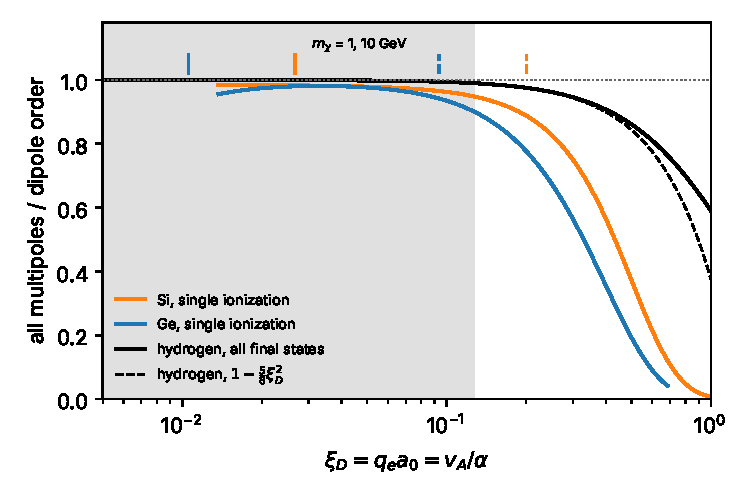
\includegraphics[width=\linewidth]{figures/ch12/limit12_2a.pdf}
\captionof{figure}{The Migdal probability with the full boost $\exp(-\ii\vect{q}_e\cdot\sum_e\vect{\rho}_e)$, all multipoles, divided by its dipole-order value, against $\xi_D = q_ea_0 = v_A/\alpha$. Black: hydrogen, all final states, $[1 - F_{1s}^2]/\xi_D^2$ from \cref{eq:6.1-P0}, exact. Dashed: its leading correction, $1 - \frac58\xi_D^2$. Orange and blue: single ionization of silicon and germanium atoms, Dirac--Hartree--Fock tables with multipoles up to $L = 10$ and at dipole order~\cite{cox2023precise}; a velocity-independent part of the tabulated full probabilities, $1.6\times10^{-4}$ (Si) and $1.3\times10^{-4}$ (Ge), which no transition between orthogonal states can have, is subtracted. Ticks: the largest recoil velocity for $\mchi = \SI{1}{GeV}$ (solid) and \SI{10}{GeV} (dashed), $v_A = 2\mu_{\chi N}v_{\mathrm{max}}/m_A$. Gray: $\xi_D \le 0.127$, where both atoms stay within \SI{10}{\percent} of the dipole result; silicon does so up to 0.188.}\label{fig:12-limit-2a}
\par}
\smallskip
Beyond $\xi_D \approx 0.13$ in germanium, reached by dark matter heavier than \SI{14}{GeV} (silicon: 0.19, \SI{9}{GeV}), an electron that is ionized can no longer leave the rest of the outer shell unexcited, and the single-ionization probability falls below the dipole value much earlier than in hydrogen.
\end{limitbox}

\noindent On the truncation label of \cref{eq:8.5-label} \cref{lim:12.2a} sits at $n_B = 2$, $n_D = 2$, $\mathfrak{M}$ = sudden and $\mathcal{K}$ = impulse. The dipole formula fails first in the outer shell, as Cox and collaborators showed. The exclusive probability of one ionization multiplies the transition of one electron by the probability that every other electron stays in its orbital. That product feels the bound--bound transitions of the outer shell at order $\xi_D^2$, with $r_{\mathrm{orb}}$ the outer-shell radius~\cite[Sect.~II\,C]{cox2023precise}. Below $\xi_D = 0.1$ all three curves of the box lie within \SI{7}{\percent} of one. The offset of about \SI{2}{\percent} of the two tabulated atoms at the smallest $\xi_D$, where the full and the dipole tables must agree, measures the numerical precision of the tables. For a particle of \SI{1}{GeV}, the endpoints are $\xi_D = 0.027$ in silicon and 0.011 in germanium, and \cref{eq:12.2-dipole} is as good as the atomic structure behind it.

\Cref{fig:12-atoms} shows the Migdal ionization spectra of silicon and germanium atoms at $E_R = \SI{1}{keV}$ against the electronic energy transfer $\omega_e$, the energy a detector records. The valence shells, bound by a few eV, dominate below a few tens of eV and fall as a power of $\omega_e$. The core shells open at their binding energies in $\omega_e$ and, because a tightly bound orbital couples to fast electrons, keep their spectrum flat up to energies of the order of their binding before they fall. The silicon $2p$ shell and the germanium $3d$ shell carry the spectrum from about \SI{50}{eV} to about a keV, and deeper shells beyond. Integrated over $\omega_e$, the ionization probability at \SI{1}{keV} is $2.09\times10^{-3}$ for silicon, of which the core shells $1s$, $2s$ and $2p$ give $7.9\times10^{-4}$, and $1.63\times10^{-3}$ for germanium in the Dirac--Hartree--Fock tables of Cox and collaborators. Xenon, from the tables of Ibe and collaborators, gives $1.98\times10^{-3}$. The three numbers are close because at fixed $E_R$ the factor $q_e^2 = 2m_e^2E_R/m_A$ falls with the mass of the atom while the dipole sum $\langle D_{\hat q}^2\rangle$ grows with the number of outer electrons. Two independent calculations exist for germanium, the relativistic local-potential one of Ibe and collaborators and the Dirac--Hartree--Fock one of Cox and collaborators. They agree within \SI{0.5}{\percent} on the $3d$ and $3p$ shells and within \SI{13}{\percent} on the valence $4p$ shell, and differ by \SI{6}{\percent} on the total, $1.73\times10^{-3}$ against $1.63\times10^{-3}$, the size of the uncertainty that the atomic structure adds.

\begin{figure}[tbp]
  \centering
  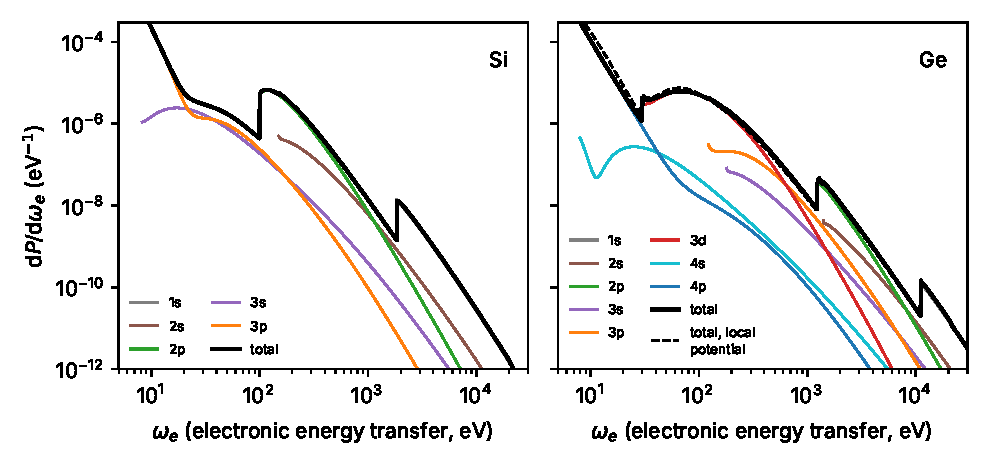
\includegraphics[width=\linewidth]{figures/ch12/fig12_2.pdf}
  \caption{Migdal ionization spectra of free silicon (left) and germanium (right) atoms at the recoil energy $E_R = \SI{1}{keV}$, per unit $\omega_e$ (electronic energy transfer), by initial shell (colors) and in total (black). Each shell is placed at $\omega_e = E_B + E_{\mathrm{ej}}$, its binding energy plus the kinetic energy of the ejected electron: measured binding energies of the core shells (\cref{sec:3.5}) and, for the valence shells, the measured first ionization energy of the atom, \SI{8.15}{eV} (Si) and \SI{7.90}{eV} (Ge), exact for the outer $p$ shell and a lower limit for the valence $s$ shell. Dipole-order Dirac--Hartree--Fock tables of Cox and collaborators~\cite{cox2023precise}, with the spin--orbit partners of each shell added, rescaled from $q_e = m_e\times10^{-3}$ to $q_e = m_e(2E_R/m_A)^{1/2}$, \SI{141}{eV} for silicon and \SI{88}{eV} for germanium. Dashed: total for germanium from the local-potential calculation of Ibe and collaborators~\cite{ibe2018migdal}, same rescaling. At other recoil energies every curve scales as $E_R$.}
  \label{fig:12-atoms}
\end{figure}

\begin{workedexample}{The Migdal probability of a germanium atom at \SI{1}{keV}}\label{we:12-germanium}
A germanium atom, $m_A = 72.630\,\mathrm{u} = \SI{67.654}{GeV}$, recoils with $E_R = \SI{1}{keV}$. Dark matter must be at least \SI{2.27}{GeV} to give it this energy at $v_{\mathrm{max}}$. The momentum transfer is $q = (2m_AE_R)^{1/2} = \SI{11.63}{MeV}$, the atom moves at $v_A = q/m_A = 1.72\times10^{-4}$, or \SI{51.5}{km.s^{-1}}, and each electron receives $q_e = m_ev_A = \SI{87.9}{eV}$, so that $q_ea_0 = v_A/\alpha = 0.024$. The tables of Ibe and collaborators are given at $q_e = m_e\times10^{-3} = \SI{511}{eV}$~\cite[Table~II]{ibe2018migdal}, and at dipole order we multiply them by $(87.9/511)^2 = 0.0296$.

The ionization probabilities are then $8.2\times10^{-4}$ from the $3d$ shell and $7.8\times10^{-4}$ from the $4p$ shell. The $3p$, $2p$ and $4s$ shells add $7.1\times10^{-5}$, $2.1\times10^{-5}$ and $1.8\times10^{-5}$, and the deeper shells less. The total is $1.73\times10^{-3}$: in this calculation one recoil in 580 ejects an electron. The shells with $n \le 3$ give $9.3\times10^{-4}$ of it. The table also lists transitions to bound orbitals. They add up to $8.75\times10^{-2}$ at the reference $q_e$, or $2.59\times10^{-3}$ at \SI{1}{keV}, more than the ionization, and the single transition $4s \to 4p$ gives $1.18\times10^{-3}$ of it. Every transition together has the probability $4.3\times10^{-3}$, one recoil in 230.

The sum rule \cref{eq:12.2-sums} checks the table. At the reference $q_e$ the exact first moment is $q_e^2N_e/2m_e = 32\times(\SI{511}{eV})^2/(2\times\SI{511}{keV}) = \SI{8.18}{eV}$. The ionization spectra, weighted with $\omega_e = E_B + E_{\mathrm{ej}}$ and the binding energies of the table, give \SI{7.28}{eV}, and the bound transitions, weighted with the differences of the tabulated level energies, \SI{0.63}{eV}. The tabulated transitions hold \SI{96.8}{\percent} of the moment; the rest lies in what the table omits, levels above $n' = 6$ and electrons faster than \SI{70}{keV}, and in the relativistic corrections to the nonrelativistic sum rule. At \SI{1}{keV} the moment is $(N_em_e/M)E_R = \SI{0.242}{eV}$, bound transitions included. Its ionization part, $\SI{7.28}{eV}\times0.0296 = \SI{0.215}{eV}$, carried by one event in 580, gives an ionizing event \SI{124}{eV} on average, and a $3d$ ionization \SI{135}{eV}.

Inside a germanium crystal the $3d$ shell keeps this probability. Its binding is \SI{29.4}{eV} below the valence maximum (\cref{sec:10.6}) where the table uses a computed \SI{35}{eV}, and the spectrum shifts with it. The valence part, $8.0\times10^{-4}$ of ionization and most of the bound transitions, does not carry over: in the crystal the $4s$ and $4p$ orbitals form the valence and conduction bands, $4s \to 4p$ is a transition across the gap, and \cref{sec:12.3} computes it from the loss function.
\end{workedexample}

\subsection{Core shells inside a crystal}\label{sec:12.2-cores}

\Cref{eq:12.2-joint} assumes three things that a crystal can violate: that the atom recoils freely, that it is isolated, and that the kick is over before the electrons respond.

\emph{Free recoil.} A nucleus bound in a lattice recoils like a free one once the recoil parameter $x_R = E_R/\langle\omega\rangle$ is large, above the impulse onset $x_R = 4$ of \cref{sec:11.4}: $q = \SI{92.5}{keV}$ and $E_R = \SI{164}{meV}$ in silicon, \SI{113}{keV} and \SI{95}{meV} in germanium. Above it the line $\omega_l = q^2/2m_A$ of \cref{eq:12.2-joint} becomes the impulse peak of \cref{eq:11.4-IA}, of relative width $x_R^{-1/2}$, $5\times10^{-3}$ at \SI{1}{keV} in germanium. The electronic factor is untouched. After the kick the neighbors pull the nucleus back on the time $1/\omega_{\mathrm{ph}}$, and the model of \cref{sec:6.1} found that this multiplies the excitation probability by $[1 - (\omega_{\mathrm{ph}}/\Delta E)^2]^{-2}$. For the germanium $3d$ shell, with the optical phonon of \SI{37.6}{meV} (\cref{tab:5-phonons}), the factor exceeds one by $3\times10^{-6}$, and for silicon $2p$ by $8\times10^{-7}$. Below the onset the lattice keeps the recoil in phonons, and the lattice factor is the multiphonon response of \cref{sec:12.4}.

\emph{Suddenness.} The kick lasts about as long as the dark matter takes to cross the nucleus, \SI{6e-21}{s} for germanium at $v_{\mathrm{max}}$ (\cref{sec:6.1}). Against the $3d$ excitation energy this is $\Delta E\,\tau_{\mathrm{acc}} = 3\times10^{-4}$, and for silicon $2p$ $7\times10^{-4}$, deep in the sudden region of \cref{fig:6-sudden}. The free atom needs no such condition, since \cref{eq:12.2-joint} is exact for it; in a crystal the condition is what lets the nucleus be treated as kicked first and decelerated afterward.

\emph{An isolated atom.} The electrons must move with their own nucleus and not with the crystal. A core orbital does. The silicon $2p$ shell has a mean radius of \SI{0.28}{\angstrom} and the germanium $3d$ shell \SI{0.39}{\angstrom}, against bonds of \SI{2.35}{\angstrom} and \SI{2.45}{\angstrom}. Their binding energies, \SI{99.5}{eV} (the spin--orbit centroid) and \SI{29.4}{eV} below the valence maximum, lie far below a valence band about \SI{12}{eV} wide. Such a shell forms a flat band whose orbitals are those of the atom, which first-principles calculations confirm for exactly these two shells (\cref{app:E.7}). The valence orbitals, of mean radius \SI{1.5}{\angstrom}, reach the neighbors, and their transitions become the band-to-band transitions of \cref{chap:10}. Their Migdal rate is the crystal formula of \cref{sec:12.3}, with the gap in place of the atomic binding. The atomic valence numbers above do not carry over: the crystal changes the valence channel by more than an order of magnitude (\cref{sec:12.3-atom}).

The mass that sets $q_e$ is $M_\kappa + \delta M_\kappa$, with the core electrons in $\delta M_\kappa$ exactly and the valence part a tensor (\cref{sec:8.6}), an effect of order $10^{-4}$. The largest correction is not in these three conditions but in the final state. Near its threshold the ejected core electron enters the conduction bands of the crystal and not the atomic continuum, and \cref{sec:10.6} found that the choice of final states changes the germanium $3d$ contribution to an electron-scattering rate by an order of magnitude near its opening. The atomic tables are reliable for core electrons ejected with tens of eV or more; within a few eV of the edge they are an estimate. With these provisos the core shells of a crystal take their Migdal probability from the atom, and \cref{sec:12.3} adds them to the valence rate.

\subsection{Excitation without ionization}\label{sec:12.2-excitation}

A kick can also leave an electron in an empty bound orbital. Kahlhoefer and Su proposed to detect this in superfluid helium, where an excited atom binds to a neighbor and the excimer emits an ultraviolet photon~\cite{kahlhoefer2026probing}. The first excited level of helium lies at \SI{20.6}{eV}, so a recoil far too weak to excite a neighbor by collision can still excite its own electrons. The probability is the sum of \cref{eq:12.2-joint} over the bound final states, and at dipole order, with the oscillator strengths \cref{eq:4.3-osc},
\begin{equation}
  P_{\mathrm{exc}} = q_e^2\sum_{f\,\mathrm{bound}}\bigl|\langle\Psi_f|D_{\hat q}|\Psi_0\rangle\bigr|^2 = \frac{q_e^2}{2m_e}\sum_{f\,\mathrm{bound}}\frac{f^{\mathrm{osc}}_{f0}}{E_f - E_0} .
  \label{eq:12.2-exc}
\end{equation}
The rate is \cref{eq:12.2-rate} with $\dd P/\dd\omega_e$ replaced by a sum of lines at the excitation energies, which is the form of Kahlhoefer and Su~\cite[Eq.~(6)]{kahlhoefer2026probing}. Only levels reached by the dipole operator appear: from the $1s^2$ ground state of helium, the $1snp\,{}^1P$ levels. With the measured oscillator strengths of these lines~\cite{kramida2024nist}, $0.276$ for $2\,{}^1P$ at \SI{21.22}{eV} and $0.073$ for $3\,{}^1P$ at \SI{23.09}{eV}, \cref{eq:12.2-exc} gives $P_{\mathrm{exc}} = 0.177\,(v_A/\alpha)^2$ for the first line, $0.220\,(v_A/\alpha)^2$ with the second, and $0.263\,(v_A/\alpha)^2$ with all lines up to the series limit at \SI{24.59}{eV}. A helium atom recoiling with \SI{10}{eV}, which dark matter of \SI{52}{MeV} can produce, has $v_A/\alpha = 0.010$ and is excited with probability $2.7\times10^{-5}$.

Any finite list of lines underestimates $P_{\mathrm{exc}}$, since every term of \cref{eq:12.2-exc} is positive; the first two helium lines hold \SI{84}{\percent} of it. A sharper statement compares the bound part with the ionization. Every bound level lies below the ionization energy $I$ and every continuum state above it. Weighting the oscillator strengths with $1/(E_f - E_0)$ therefore favors the bound part. Let $F_{\mathrm{exc}}$ and $F_{\mathrm{ion}}$ be the oscillator strength in the bound lines and in the continuum, and $P_{\mathrm{ion}} = P_{\mathrm{Mig}} - P_{\mathrm{exc}}$ the ionization probability. Then $P_{\mathrm{exc}} \ge q_e^2F_{\mathrm{exc}}/2m_eI$ and $P_{\mathrm{ion}} \le q_e^2F_{\mathrm{ion}}/2m_eI$, and
\begin{equation}
  \frac{P_{\mathrm{exc}}}{P_{\mathrm{ion}}} \ge \frac{F_{\mathrm{exc}}}{F_{\mathrm{ion}}} .
  \label{eq:12.2-bound}
\end{equation}
An estimate of the bound share from the oscillator strength alone, the share of the Thomas--Reiche--Kuhn sum \cref{eq:4.3-TRK} in the lines, is a lower bound. For hydrogen the lines hold 0.565 of the oscillator strength (\cref{sec:4.3}) but 0.717 of the dipole probability, of which the $2p$ level gives 0.555 and the levels with $n \le 3$ give 0.644.

\begin{limitbox}[Migdal excitation of bound final states][lim:12.2b]
A free atom recoiling with $q$ is left in the bound level $f$ with $P_f = |\langle\Psi_f|\exp(-\ii\vect{q}_e\cdot\sum_e\vect{\rho}_e)|\Psi_0\rangle|^2$, and the rate is the free-recoil rate times $\sum_fP_f\,\delta(\omega_e - E_f + E_0)$ over a list of levels~\cite[Eqs.~(1) and (6)]{kahlhoefer2026probing}; at dipole order this is \cref{eq:12.2-exc}.
\par\smallskip
{\centering
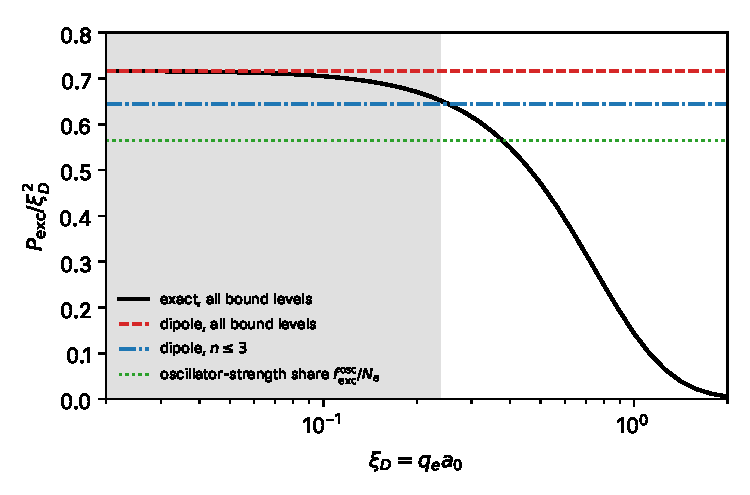
\includegraphics[width=\linewidth]{figures/ch12/limit12_2b.pdf}
\captionof{figure}{Probability that a kick leaves a hydrogen atom in a bound excited level, divided by $\xi_D^2 = (q_ea_0)^2$, against $\xi_D$. Solid: exact, the full boost and every bound level, from radial integrals with the spherical Bessel functions $j_\ell(q_er)$ for $n \le 40$ and $\ell \le 12$ and an $n^{-3}$ tail. Dashed: dipole order, all $np$ levels, 0.717. Dash-dotted: dipole order, levels with $n \le 3$ only, 0.644. Dotted: the bound share of the oscillator strength times the total dipole probability, 0.565, the lower bound \cref{eq:12.2-bound}. Gray: $\xi_D \le 0.24$, where the dipole sum over all levels is within \SI{10}{\percent} of the exact result.}\label{fig:12-limit-2b}
\par}
\smallskip
Beyond $\xi_D \approx 0.24$ the boost carries the electron more and more into the continuum, and the dipole sum overstates the bound probability, which falls to a fifth of it at $\xi_D = 1$.
\end{limitbox}

\noindent \Cref{lim:12.2b} sits at $n_B = 2$, $n_D = 2$, $\mathfrak{M}$ = sudden and $\mathcal{K}$ = impulse, as \cref{lim:12.2a} does. For dark matter lighter than \SI{1}{GeV} in helium, $\xi_D$ stays below 0.16, where the dipole sum for hydrogen is within \SI{4}{\percent} of the exact one; the finite list of lines, \SI{16}{\percent} short in helium, sets the larger error of the published estimate.

In germanium the bound transitions outnumber the ionizations. The table of \cref{we:12-germanium} lists $8.75\times10^{-2}$ in bound transitions against $5.86\times10^{-2}$ in ionization at the reference $q_e$, mostly $4s \to 4p$ and $4p \to 4d,\,5s$, and since the table stops at $n' = 6$ the true bound share is larger still. In a crystal these valence transitions do not exist as such. The bound final states of a crystal are excitons, whose lines below the pair continuum carry as much weight as the free pairs within $8E_x^b$ of the edge would (\cref{sec:10.5}). The Migdal entry \cref{eq:12.1-Skk} weights each final state with $\omega_e^{-4}$, which favors the lines below the edge for the same reason as \cref{eq:12.2-bound}. The exciton share of the Migdal spectrum is therefore at least the share of the lines in the electronic response near the edge. In silicon, with $E_x^b = \SI{14.7}{meV}$, and in germanium, whose indirect exciton is bound by about \SI{5}{meV}~\cite{macfarlane1957fine}, that share is negligible. In wide-gap crystals with binding energies of an eV and more it is not, and the lines are a separate, optically detectable signal (\cref{app:E.15}).

\section{The loss-function Migdal probability}\label{sec:12.3}

A dark-matter particle of \SI{300}{MeV} can give a silicon nucleus a momentum of \SI{1.6}{MeV} and a recoil energy of \SI{47}{eV}. The momentum is seven hundred times the size of the Brillouin zone, the recoil energy a thousand times that of a phonon, and the nucleus leaves its site as a free particle (\cref{sec:11.4}). The electrons it sets in motion take a momentum of a few keV, and half of the time they receive less than \SI{4.6}{eV}, a few times the gap. In this regime the Migdal entry \cref{eq:12.1-Skk} of the joint response simplifies twice. The lattice factor collapses to a free recoil, and the electronic factor becomes the loss function $L(\vect{p},\omega_e)$ that \cref{sec:10.2} used for the electron-recoil rate. The probability that a kick leaves an electron--hole pair is then fixed by one material function, an integral of $L$ over momenta weighted by $\omega_e^{-4}$, and it comes out thirty times larger in crystalline silicon than in a silicon atom. The same function sets the rate per unit target mass, which \cref{sec:17.5} uses to compare materials.

\subsection{Migdal probability through the loss function}\label{sec:12.3-soft}

Three approximations take \cref{eq:12.1-Skk} to the loss function: the diagonal $\vect{G} = \vect{G}'$ of the electronic factor, a free recoil, and the soft limit $p \ll q$. On the diagonal the integral over the zone and the sum over $\vect{G}$ then combine into one integral over the unreduced momentum $\vect{p} = \vect{k} + \vect{G}$ given to the electrons. By \cref{eq:4.4-SL}, with the diagonal inverse dielectric matrix \cref{eq:E.6-L}, the diagonal element of the density response at $\vect{p}$ is the loss function at that momentum:
\begin{equation}
  S^{ee}_{\vect{G}\vect{G}}(\vect{k},\omega_e) = \frac{2p^2}{e^2}\,L(\vect{p},\omega_e) , \qquad \omega_e > 0,\; T \ll \Eg .
  \label{eq:12.3-See}
\end{equation}
The local fields on the diagonal stay inside $L$; the dropped elements $\vect{G} \ne \vect{G}'$ carry the part of the local fields that couples different momenta, and we return to both parts of the local fields below. The free recoil treats each nucleus as if it were alone and in the impulse regime, so that the lattice factor is the free recoil of \cref{sec:11.4} at the momentum $\vect{q} - \vect{p}$ the nucleus keeps, $S^{\mathrm{ad}}_{\kappa}(\vect{q} - \vect{p},\omega_l) = 2\pi\nd_\kappa\,\delta(\omega_l - |\vect{q} - \vect{p}|^2/2M_\kappa)$. The \emph{soft limit} $p \ll q$ says that the electrons take a small part of the momentum. The lattice factor then becomes $2\pi\nd_\kappa\,\delta(\omega_l - E_R)$ with $E_R = q^2/2M_\kappa$, and it no longer depends on $\vect{p}$. The Migdal entry then factorizes into the free recoil and a probability per kick,
\begin{equation}
  S_{\kappa\kappa}(\vect{q};\omega_l,\omega_e) = 2\pi\nd_\kappa\,\delta(\omega_l - E_R)\,\frac{\dd P_{\mathrm{Mig}}}{\dd\omega_e} .
  \label{eq:12.3-factor}
\end{equation}

The vertex is the potential of the moving ion. In silicon the ten electrons of the $1s$, $2s$ and $2p$ shells are bound by \SI{100}{eV} or more and follow their nucleus; for the valence electrons whose response is $L$, nucleus and core act together as one ion. The potential of this ion is
\begin{equation}
  v_\kappa(\vect{p}) = -\frac{Z_{\mathrm{ion}}(p)\,e^2}{p^2} , \qquad Z_{\mathrm{ion}}(p) = Z_\kappa - f^{\mathrm{core}}_\kappa(p) ,
  \label{eq:12.3-Zion}
\end{equation}
with $f^{\mathrm{core}}_\kappa(p)$ the form factor of the core electrons, the Fourier transform of their density. \Cref{eq:12.3-Zion} defines the \emph{valence ionization factor} $Z_{\mathrm{ion}}(p)$. At small $p$ it is the ionic charge, 4 for silicon; at large $p$ the probe resolves the core and $Z_{\mathrm{ion}}$ rises toward the nuclear charge 14. With the core orbitals of the free atom from \cref{sec:3.5}, $Z_{\mathrm{ion}}$ of silicon exceeds 4 by \SI{5}{\percent} at \SI{2.4}{keV} and by \SI{10}{\percent} at \SI{3.4}{keV}, and reaches 4.84 at \SI{5}{keV} and 6.78 at \SI{10}{keV}. The split between core and valence is a convention, and $Z_{\mathrm{ion}}$ must count exactly the electrons that $L$ leaves out.

When \cref{eq:12.3-See,eq:12.3-Zion} and the lattice factor are inserted in \cref{eq:12.1-Skk}, the factors combine as
\begin{equation*}
  \frac{1}{2\pi}\,\frac{(\vect{q}\cdot\vect{p})^2}{M_\kappa^2\omega_e^4}\,\frac{Z_{\mathrm{ion}}^2e^4}{p^4}\,\frac{2p^2}{e^2}\,L\;2\pi\nd_\kappa
  = 2\pi\nd_\kappa\,\frac{e^2}{\pi}\,\frac{Z_{\mathrm{ion}}^2(\vect{v}_N\cdot\vect{p})^2}{\omega_e^4\,p^2}\,L ,
\end{equation*}
with $\vect{v}_N = \vect{q}/M_\kappa$ the recoil velocity of \cref{sec:6.1}. Since $e^2/\pi = 4\alpha$, comparison with \cref{eq:12.3-factor} gives the result.
\begin{keyresult}[The crystal Migdal probability in the soft limit]
For a kick of momentum $\vect{q}$ in the impulse regime, with $p \ll q$, the probability per unit electronic energy that a nucleus of species $\kappa$ leaves the valence electrons excited is
\begin{equation}
  \frac{\dd P_{\mathrm{Mig}}}{\dd\omega_e} = 4\alpha\int\frac{\dd^3p}{(2\pi)^3}\;Z_{\mathrm{ion}}(p)^2\,\frac{(\vect{v}_N\cdot\vect{p})^2}{\omega_e^4\,p^2}\,L(\vect{p},\omega_e)
  = \frac{4\alpha v_N^2}{3\,\omega_e^4}\,L_{\mathrm{Mig}}(\omega_e) ,
  \label{eq:12.3-soft}
\end{equation}
where the second form holds for a direction-averaged loss function and defines the Migdal-weighted loss function
\begin{equation}
  L_{\mathrm{Mig}}(\omega_e) = \int\frac{\dd^3p}{(2\pi)^3}\;Z_{\mathrm{ion}}(p)^2\,\bar L(p,\omega_e) .
  \label{eq:12.3-LMig}
\end{equation}
\end{keyresult}
\noindent This is the formula of Knapen, Kozaczuk and Lin~\cite[Eq.~(6)]{knapen2021migdal}. Read as a product, it is the probability of a dipole boost, $v_N^2$, times the response of the electrons to the field of a charge $Z_{\mathrm{ion}}$ that has suddenly started to move. The screening and the local fields of \cref{sec:10.2} enter here unchanged. The factor $\omega_e^{-4}$ is the square of the boost denominator $\omega_e^2$ of \cref{eq:12.1-amp}. With $v_N^2 = 2E_R/M_\kappa$ the probability grows linearly with the recoil energy, and the material enters only through $L_{\mathrm{Mig}}$.

For silicon we evaluate \cref{eq:12.3-soft} with the loss function of Knapen, Kozaczuk and Lin with local fields~\cite{knapen2021dark}, which is the table of \cref{sec:10.2}. We count the table from \SI{1.11}{eV}, the step-model gap that accompanies it, rather than from its scissor gap, the physical \SI{1.17}{eV}; the table stops at \SI{89}{eV} and \SI{22.5}{keV}. At $E_R = \SI{100}{eV}$, reached at $q = \SI{2.29}{MeV}$ with $v_N = 8.74\times10^{-5}$ (\SI{26}{km/s}), the probability is $P_{\mathrm{Mig}} = 6.1\times10^{-3}$, or $6.1\times10^{-5}$ per eV of recoil energy. Half of the probability lies below $\omega_e = \SI{4.6}{eV}$ and \SI{89}{\percent} below \SI{10}{eV}; the mean is \SI{6.0}{eV}. The momenta are larger than the zone: the median $p$ is \SI{5.7}{keV}, two and a half times $q_{\mathrm{BZ}}$ of \cref{eq:11.1-qBZ}, and \SI{97}{\percent} of the probability comes from $p > q_{\mathrm{BZ}}$. The plasmon, at $p \lesssim \SI{2.5}{keV}$, carries \SI{4}{\percent}: the factor $\omega_e^{-4}$ favors the single-pair continuum near the gap over the plasmon at \SI{17}{eV}. With a point ion of charge 4 instead of $Z_{\mathrm{ion}}(p)$ the probability falls to $3.9\times10^{-3}$, lower by a factor 1.57.

\begin{workedexample}{The coefficient $4\alpha$ from the f-sum}\label{we:12-fsum}
The coefficient of \cref{eq:12.3-soft} can be checked without the diagrams of \cref{eq:12.1-Skk}, from a sum rule. Take one Fourier component $\vect{p}$ of the force of the ion, $F_{\vect{p}} = \vect{v}_N\cdot\nabla_{\vect{X}}V_{eN}$ restricted to that component. By \cref{eq:12.1-force} it is $-\ii(\vect{v}_N\cdot\vect{p})\,v_\kappa(\vect{p})\,n_e(\vect{p})/\Vol$ up to a phase, and the Migdal amplitude to a final state $j$ is $\langle\Psi_j|F_{\vect{p}}|\Psi_0\rangle/\Delta E_j^2$. The fifth moment of the probability weighs each final state with $\Delta E_j^5$ and therefore equals the energy-weighted sum $\sum_j\Delta E_j|\langle\Psi_j|F_{\vect{p}}|\Psi_0\rangle|^2$. For the density operator this sum is the f-sum rule \cref{eq:4.3-fsum}, $\sum_j\Delta E_j|\langle\Psi_j|n_e(\vect{p})|\Psi_0\rangle|^2 = N_ep^2/2m_e$ at $T = 0$, which holds for the interacting electrons exactly. Per unit volume the fifth moment is therefore
\begin{equation*}
  (\vect{v}_N\cdot\vect{p})^2\,|v_\kappa(\vect{p})|^2\,\frac{\nd_e\,p^2}{2m_e} = (\vect{v}_N\cdot\vect{p})^2\,\frac{Z_{\mathrm{ion}}^2e^4}{p^4}\,\frac{\nd_e\,p^2}{2m_e} .
\end{equation*}
The loss-function form with an unknown coefficient $c$ in place of $4\alpha$ gives instead, with the f-sum of the loss function $\int_0^\infty\dd\omega\,\omega L = (\pi/2)\omega_p^2$ (\cref{eq:10.2-moments}) and $\omega_p^2 = e^2\nd_e/m_e$,
\begin{equation*}
  c\,Z_{\mathrm{ion}}^2\,\frac{(\vect{v}_N\cdot\vect{p})^2}{p^2}\int_0^\infty\dd\omega\,\omega L = c\,Z_{\mathrm{ion}}^2\,\frac{(\vect{v}_N\cdot\vect{p})^2}{p^2}\,\frac{\pi}{2}\,\frac{e^2\nd_e}{m_e} .
\end{equation*}
The two fifth moments agree if $c = e^2/\pi = 4\alpha$, at every $\vect{p}$ and for any electron density.

For silicon the check also measures the table. At the valence density, $\nd_e = \SI{2.00e23}{cm^{-3}}$ and $\omega_p^{\mathrm{val}} = \SI{16.6}{eV}$, the table holds 0.94, 0.93, 0.92 and 0.90 of the f-sum at $p = 1$, 2, 3 and \SI{5}{keV}, so the fifth moment of the computed spectrum is within \SI{10}{\percent} of its exact value there. At \SI{7.5}{keV} the table holds 0.62 and at \SI{10}{keV} only 0.17, because the free-electron peak $p^2/2m_e$ moves past the table's last energy of \SI{89}{eV}. The probability is far less sensitive than the fifth moment, since $\omega_e^{-4}$ weights the low energies the table does contain. The momenta above \SI{10}{keV} give \SI{2.3}{\percent} of $P_{\mathrm{Mig}}$, and an upper bound on the energies beyond the table follows from the same sum rule, $\int_{\omega_{\mathrm{top}}}^\infty\dd\omega\,L/\omega^4 \le (\pi/2)\omega_p^2/\omega_{\mathrm{top}}^5$. At $\omega_{\mathrm{top}} = \SI{89}{eV}$, summed over the momenta of the table, the bound is \SI{1.6}{\percent} of the probability below $\omega_{\mathrm{top}}$.
\end{workedexample}

The material input of \cref{eq:12.3-soft} is the loss function of the valence electrons at momenta up to about \SI{20}{keV}, where the Migdal weight ends, and energies from the gap to about \SI{50}{eV}. At these momenta the calculation needs the diagonal elements far from the head; \cref{sec:10.2} met the same requirement for electron recoil. An all-electron calculation of $L$ at $p \le \SI{30}{keV}$ removes the need for $Z_{\mathrm{ion}}$ and puts the core shells in the same table. The random-phase loss function does not contain the Migdal lines of excitons below the gap.

\subsection{Validity of the soft limit}\label{sec:12.3-validity}

Knapen and collaborators state \cref{eq:12.3-soft} with the scalar dielectric function $\varepsilon(\vect{p},\omega)$ and note that it holds only for $\vect{p}$ in the first zone~\cite[text after Eq.~(6)]{knapen2021migdal}. Inside the zone the scalar function is the macroscopic one, and the loss function is the head of the inverse matrix. Outside it, a scalar function of $|\vect{p}|$ has no unique meaning, and the derivation above says which element to take: the diagonal element of the inverse at the reciprocal vector that contains $\vect{p}$. The distinction matters because the Migdal weight lies outside the zone. \Cref{lim:12.3a} compares, momentum by momentum, the loss function that a scalar random-phase $\varepsilon$ gives with the diagonal element of the inverse with local fields. The two agree within \SI{10}{\percent} up to $p = 1.3\,q_{\mathrm{BZ}} = \SI{2.9}{keV}$, which holds \SI{8}{\percent} of the probability. Beyond, the scalar function overestimates the weight by \SI{24}{\percent} at $2q_{\mathrm{BZ}}$ and \SI{35}{\percent} at $3q_{\mathrm{BZ}}$, where the probability peaks, and the total by a factor 1.35. The mechanism is the one of \cref{sec:10.2}: at $|\vect{p}| \approx 2$--$3\,|\vect{G}_{111}|$ the charge induced in the cell has a macroscopic component that screens the field of the ion.
\begin{limitbox}[Crystal Migdal effect through the loss function][lim:12.3a]
$\dd P/\dd\omega = 4\alpha\int\dd^3p/(2\pi)^3\,Z_{\mathrm{ion}}(p)^2|\vect{v}_N\cdot\vect{p}|^2\,\Imag[-1/\varepsilon(\vect{p},\omega)]/(\omega^4p^2)$ with a scalar dielectric function, for $\vect{p}$ in the first zone~\cite[Eq.~(6)]{knapen2021migdal}.
\par\smallskip
{\centering
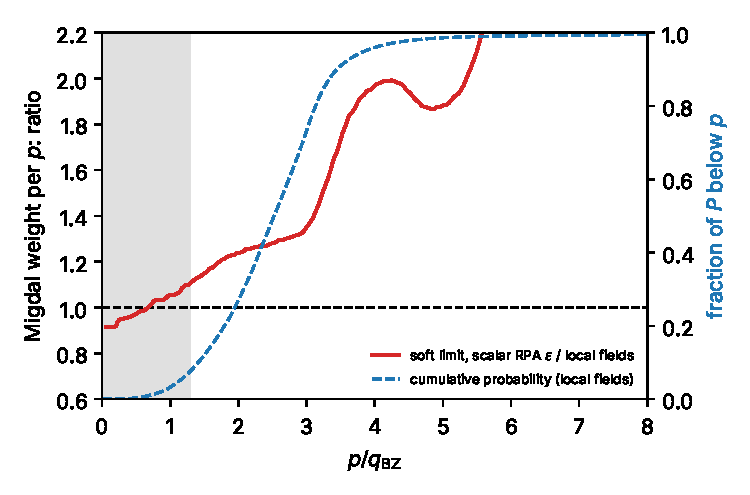
\includegraphics[width=\linewidth]{figures/ch12/limit12_3a.pdf}
\captionof{figure}{Migdal weight of silicon per unit momentum $p$ given to the electrons, $p^2Z_{\mathrm{ion}}(p)^2\int_{\Eg}\dd\omega\,L(p,\omega)/\omega^4$, from the loss function of a scalar random-phase dielectric function at $|\vect{p}|$ (no local fields), divided by the same with the diagonal element of the inverse dielectric matrix with local fields, against $p/q_{\mathrm{BZ}}$ ($q_{\mathrm{BZ}} = \SI{2.25}{keV}$). Both from the direction-averaged tables of Knapen, Kozaczuk and Lin~\cite{knapen2021dark} (threshold \SI{1.11}{eV}, the step-model gap that accompanies them, $\omega \le \SI{89}{eV}$), smoothed over \SI{0.7}{keV} in $p$; $Z_{\mathrm{ion}}(p)$ of \cref{eq:12.3-Zion}. The elements $\vect{G} \neq \vect{G}'$ are in neither curve. Dashed, right axis: the fraction of $P_{\mathrm{Mig}}$ carried by momenta below $p$. Gray band: $p \le 1.3\,q_{\mathrm{BZ}}$, where the two agree within \SI{10}{\percent}; it holds \SI{8}{\percent} of the probability.}\label{fig:12-limit-3a}
\par}
\smallskip
Beyond the first zone the scalar form has to be replaced by the diagonal of the inverse dielectric matrix, and the local fields lower the silicon probability by a factor 1.35; the elements $\vect{G} \neq \vect{G}'$ are the next correction.
\end{limitbox}

The elements $\vect{G} \neq \vect{G}'$ keep the full matrix in \cref{eq:12.1-Skk}. For a direction-averaged target the boost factor averages to $\langle[\hat{\vect{q}}\cdot(\vect{k}+\vect{G})][\hat{\vect{q}}\cdot(\vect{k}+\vect{G}')]\rangle = (\vect{k}+\vect{G})\cdot(\vect{k}+\vect{G}')/3$. At the random-phase level the response matrix is $S^{ee}_{\vect{G}\vect{G}'} = (2|\vect{k}+\vect{G}||\vect{k}+\vect{G}'|/e^2)\,\Imag[-(\tilde\varepsilon^{-1})_{\vect{G}\vect{G}'}]$, with the symmetrized matrix $\tilde\varepsilon_{\vect{G}\vect{G}'} = \delta_{\vect{G}\vect{G}'} - v_{\mathrm{C}}^{1/2}(\vect{k}+\vect{G})\,R^0_{\vect{G}\vect{G}'}(\vect{k},\omega)\,v_{\mathrm{C}}^{1/2}(\vect{k}+\vect{G}')$, which has the same inverse diagonal as $\varepsilon$. In a crystal with time reversal and inversion it is symmetric, $\tilde\varepsilon_{\vect{G}\vect{G}'} = \tilde\varepsilon_{\vect{G}'\vect{G}}$, but not Hermitian at frequencies where the crystal absorbs; $\Imag[-(\tilde\varepsilon^{-1})_{\vect{G}\vect{G}'}]$ denotes the anti-Hermitian part $[(\tilde\varepsilon^{-1})^\dagger - \tilde\varepsilon^{-1}]_{\vect{G}\vect{G}'}/2\ii$, which for a symmetric matrix is the imaginary part element by element. With a constant ion charge, $L_{\mathrm{Mig}}$ of \cref{eq:12.3-LMig} becomes
\begin{equation}
  \begin{aligned}
  L_{\mathrm{Mig}}(\omega) &= \frac{Z_{\mathrm{ion}}^2}{\Omega}\,\mathcal{F}_{\mathrm{Mig}}(\omega) , \\
  \mathcal{F}_{\mathrm{Mig}}(\omega) &= \sum_{\vect{G}\vect{G}'}\int_{\mathrm{BZ}}\frac{\Omega\,\dd^3k}{(2\pi)^3}\,\frac{(\vect{k}+\vect{G})\cdot(\vect{k}+\vect{G}')}{|\vect{k}+\vect{G}|\,|\vect{k}+\vect{G}'|}\,\ee^{\ii(\vect{G}-\vect{G}')\cdot\vect{\tau}_\kappa}\,\Imag\bigl[-(\tilde\varepsilon^{-1})_{\vect{G}\vect{G}'}(\vect{k},\omega)\bigr] ,
  \end{aligned}
  \label{eq:12.3-FL}
\end{equation}
where $\vect{\tau}_\kappa$ is the position of the struck nucleus in the cell, averaged over the equivalent sites of its species. The indices are in the order of $S^{ee}_{\vect{G}\vect{G}'}$ in \cref{eq:12.1-Skk}, with $n_e(\vect{k}+\vect{G})^\dagger$ on the left of $R^0_{\vect{G}\vect{G}'}$; the transposed order reverses the sign of the phase. The reversal leaves silicon unchanged, since its two sites are images under inversion, but not GaAs. The phase belongs to the struck nucleus: the off-diagonal elements depend on where the origin of $\varepsilon$ is placed, and the phase is one only when the origin sits on that atom. The diagonal terms carry no phase and give back \cref{eq:12.3-LMig} at any origin. The off-diagonal terms need the full matrix, which the tables of \cref{sec:10.2} do not contain. In an empirical-pseudopotential random-phase model of silicon, with the phase of \cref{eq:12.3-FL}, the full matrix exceeds the diagonal form on the total by a factor of 1.38 with $8^3$ points $\vect{k}$ and $|\vect{G}|^2 \le 19\,(2\pi/a)^2$ and of about 1.2 when extrapolated in both. The two numbers are not a bracket: the factor still falls as reciprocal-lattice vectors are added, and the fall is not slowing, so 1.2 is not a lower bound. The off-diagonal elements raise the rate at every truncation computed, and the factor is flat in $\mchi$. The model carries only about two thirds of the diagonal local-field effect of \cref{lim:12.3a}, so its off-diagonal size is a guide, not a bound in either direction. The full local-field calculation that would replace the model estimate is open.

The free recoil is the second approximation. Below the impulse onset of \cref{sec:11.4}, $x_R = 4$ at $q = \SI{92.5}{keV}$ in silicon, the lattice takes the recoil as single phonons and multiphonons, not as a free particle. In the soft limit, however, the lattice factor drops out of the probability. It enters the rate only through the energy balance $\omega = \omega_e + \omega_l$ in $\vmin$, and the lattice energy has the mean $E_R$ in every regime (\cref{eq:5.6-sum}) and is small against $\omega_e$: \SI{0.16}{eV} at the onset, against a few eV. Replacing the free recoil by the incoherent response of a bound silicon nucleus at all phonon orders, including its zero-phonon line, changes the rate by less than $10^{-5}$ at every mass from 3 to \SI{110}{MeV} (\cref{lim:12.3b}). The impulse onset is therefore not where the Migdal formula fails.

Dropping $\vect{p}$ from the lattice factor, the soft limit as defined above, leaves the electronic spectrum unchanged, because the lattice factor has unit weight at every $\vect{q} - \vect{p}$ (\cref{sec:12.4}). The boost amplitude remains to be examined, and it expands in $v_Np/\omega_e$, not in $p/q$. For a free nucleus the kick and the Coulomb exchange with the electrons come in two time orderings~\cite[Eq.~(1)]{liang2021describing}. Kicked first, the nucleus moves with $\vect{q}$, passes $\vect{p}$ to the electrons and leaves with $\vect{q} - \vect{p}$; the energy denominator is $\omega_e - b + a$, with $b = \vect{q}\cdot\vect{p}/M_\kappa$ and $a = p^2/2M_\kappa$. With the exchange first, the nucleus recoils with $-\vect{p}$ before the kick, and the denominator is $\omega_e + a$. The boost factor $(\vect{v}_N\cdot\vect{p})/\omega_e^2$ becomes
\begin{equation}
  \frac{1}{\omega_e - b + a} - \frac{1}{\omega_e + a} = \frac{b}{(\omega_e - b + a)(\omega_e + a)} = \frac{b}{\omega_e^2}\Bigl(1 + \frac{b - 2a}{\omega_e} + \cdots\Bigr) ,
  \label{eq:12.3-bracket}
\end{equation}
the free-nucleus case of \cref{eq:12.4-exact}. The numerator of \cref{eq:12.3-bracket} is $\vect{q}\cdot\vect{p}/M_\kappa$ at every $p$: the velocity in the boost is that of the kicked nucleus, whatever momentum the electrons take. Averaged over the angle $c$ between $\vect{q}$ and $\vect{p}$, the square gives
\begin{equation*}
  \Bigl\langle\frac{b^2}{(\omega_e - b + a)^2(\omega_e + a)^2}\Bigr\rangle = \frac{v_N^2p^2}{3\omega_e^4}\Bigl[1 - \frac{2p^2}{M_\kappa\omega_e} + \frac95\,\frac{v_N^2p^2}{\omega_e^2} + \cdots\Bigr] ,
\end{equation*}
the free-nucleus part of \cref{eq:12.4-corr}. The terms odd in $c$ drop out; in a crystal they drop out because the loss function is even under $\vect{p} \to -\vect{p}$ in any target with time reversal. There is no term in $p/q$, so the soft limit does not fail when the electrons take a momentum comparable with the kick. The recoil term $2p^2/M_\kappa\omega_e$ is $2\times10^{-3}$ at the median $p$ near the gap. The Doppler term $\tfrac95v_N^2p^2/\omega_e^2$ grows with the recoil energy; it is the shift $\vect{v}_N\cdot\vect{p}$ of the electronic energy by the moving nucleus, taken at second order. Weighted with the silicon spectrum, the Doppler term is 0.04 at $E_R = \SI{100}{eV}$, 0.13 at \SI{300}{eV} and 0.42 at \SI{1}{keV}. It is only the leading term. Near the gap $v_Np/\omega_e$ is already 0.41 at the median $p$ and $E_R = \SI{100}{eV}$, and the higher orders of \cref{eq:12.3-bracket} add as much again. With the exact bracket the soft-limit probability is low by the factor 0.93 at \SI{100}{eV}, 0.79 at \SI{300}{eV} and 0.62 at \SI{500}{eV}, whereas the leading term alone gives 0.96, 0.90 and 0.85. The soft limit holds within \SI{10}{\percent} up to $E_R \approx \SI{160}{eV}$, the spectrum-weighted counterpart of the bound $v_Np/\omega_e \le 0.27$ found near the gap at fixed $p$ in \cref{lim:12.4a}. Toward \SI{1}{keV} the expansion breaks down. There $v_Np$ at the median momentum is \SI{1.6}{eV}, above the gap, and the denominator $\omega_e - b + a$ vanishes inside the range of the integral: the kicked nucleus, already moving, ionizes the electrons as a slow ion does. Ionization by the already moving nucleus is an on-shell two-step process, the electronic stopping of the recoiling ion, not a Migdal transition, and the second-order amplitude does not describe it. The momenta where the denominator vanishes hold \SI{0.9}{\percent} of the soft-limit probability at \SI{500}{eV} and \SI{3.7}{\percent} at \SI{1}{keV}.
\begin{limitbox}[Crystal Migdal rate with free recoil][lim:12.3b]
$\mathcal{R} = (\rho_\chi/\mchi)\,[2A^2\sigma_p\,Z_{\mathrm{ion}}^2\,\alpha N_T/(3\mu_{\chi n}^2\Omega M^2)]\int\dd^3v\,(f/v)\int p_N^3\,\dd p_N\int\dd\omega\,\omega^{-4}\,\Theta(v - \vmin)\,\mathcal{F}_{\mathrm{Mig}}(\omega)$, $\vmin = p_N/2\mu_{\chi N} + \omega/p_N$, with $N_T$ the number of nuclei per unit target mass, $\Omega$ the cell volume, $p_N$ the momentum transfer, the soft-limit amplitude and $\mathcal{F}_{\mathrm{Mig}}$ of \cref{eq:12.3-FL}~\cite[Eqs.~(1), (7), (11), (12)]{liang2021describing}.
\par\smallskip
{\centering
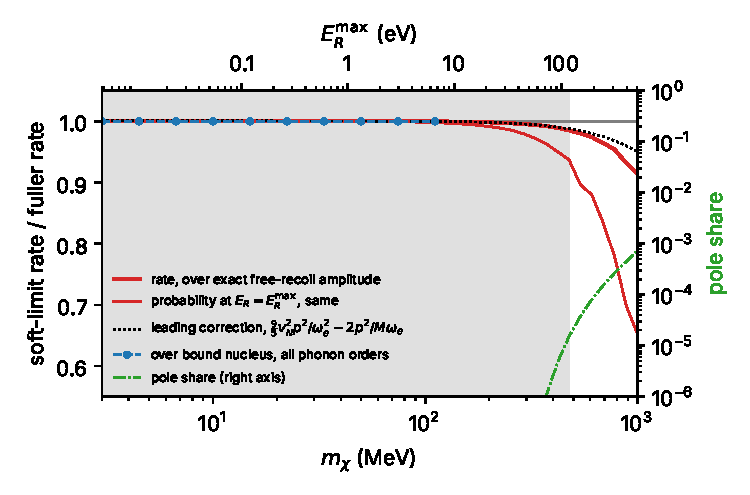
\includegraphics[width=\linewidth]{figures/ch12/limit12_3b.pdf}
\captionof{figure}{Total Migdal rate of silicon ($\omega_e \ge \SI{1.11}{eV}$, heavy mediator) in the soft limit with a free recoil, divided by two fuller results, against the dark-matter mass; top axis, the largest recoil energy $E_R^{\max} = 2\mu_{\chi N}^2v_{\mathrm{max}}^2/M$. Thick solid: over the rate with the exact free-recoil amplitude \cref{eq:12.3-bracket}. Thin solid: the same ratio for the probability at $E_R = E_R^{\max}$, the end of the recoil spectrum. Dotted: the leading correction $\frac95v_N^2p^2/\omega_e^2 - 2p^2/M_\kappa\omega_e$ alone. Dashed with points: over the soft-limit rate with the incoherent response of a bound nucleus at all phonon orders and $T = 0$ (density of states of \cref{sec:5.2}); it differs from one by less than $10^{-5}$. Dash-dotted, right axis: the share of the soft-limit rate at momenta where the exact amplitude has a pole, $v_Np \ge \omega_e + p^2/2M_\kappa$, which both rates of the ratio leave out. Every curve uses the same diagonal loss function with local fields and $Z_{\mathrm{ion}}(p)$ in place of $\mathcal{F}_{\mathrm{Mig}}$, and the halo of \cref{sec:1.2}. Gray band: $\mchi \lesssim \SI{0.5}{GeV}$, where the probability at the end of the recoil spectrum is within \SI{10}{\percent} of the exact one.}\label{fig:12-limit-3b}
\par}
\smallskip
Above about \SI{0.5}{GeV} the end of the recoil spectrum passes $E_R \approx \SI{160}{eV}$, where the motion of the nucleus during the electronic transition changes the probability by more than \SI{10}{\percent}, and near \SI{1}{keV} the moving nucleus ionizes the electrons by itself; the binding of the nucleus changes the soft-limit rate by less than $10^{-5}$ at every mass from 3 to \SI{110}{MeV}.
\end{limitbox}

\noindent From 3 to \SI{150}{MeV} the soft-limit rate is within $1.1\times10^{-3}$ of the exact free-recoil rate, and at \SI{1}{GeV}, where the rate integrates over the whole recoil spectrum, it is low by the factor 0.91.

Below the onset the bound amplitude of \cref{sec:12.4} stays within a few parts in $10^3$ of the soft limit (\cref{eq:12.4-corr}). At low mass, therefore, neither the soft limit nor the lattice limits the formula; the electronic factor does (\cref{lim:12.3a}).

The core shells stay frozen in $Z_{\mathrm{ion}}$. Their own excitation is a separate Migdal process of atomic type, with the boost of each core shell (\cref{sec:12.2}). The $2p$ shell of an isolated silicon atom gives $7.1\times10^{-5}$ at $E_R = \SI{100}{eV}$, \SI{1.2}{\percent} of the valence probability, at $\omega_e$ above \SI{100}{eV}. And the formula needs no restriction to $\mchi \ll M_\kappa$: the reduced mass $\mu_{\chi N}$ in $\vmin$ keeps the recoil of a heavy particle, and only the per-mass form below drops it.

\subsection{Crystal and atomic spectra of silicon}\label{sec:12.3-atom}

The crystal formula and the atomic formula of \cref{sec:12.2} answer the same question for the same nucleus, and they differ by more than an order of magnitude. \Cref{fig:12-crystal-atom} shows both at $E_R = \SI{100}{eV}$. The crystal probability is $6.1\times10^{-3}$. The isolated silicon atom, with all its shells and the Dirac--Hartree--Fock tables of Cox and collaborators~\cite{cox2023precise}, gives $2.1\times10^{-4}$, of which $1.3\times10^{-4}$ come from the $3s$ and $3p$ valence shells. The crystal is 29 times the whole atom and 47 times its valence shells.

\begin{figure}[tbp]
  \centering
  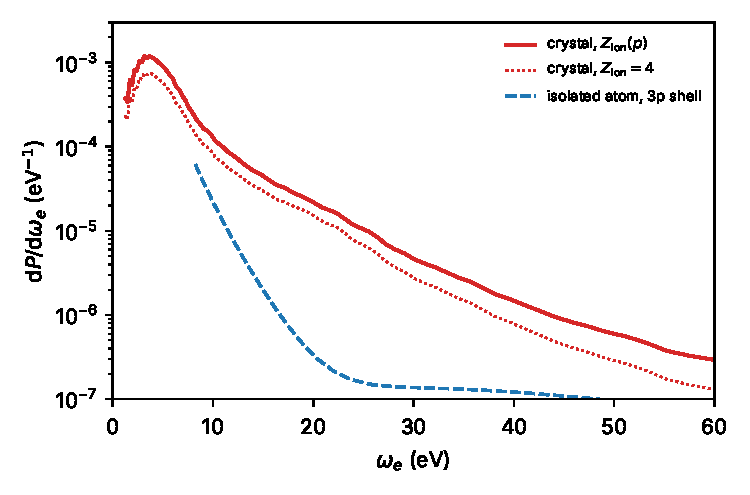
\includegraphics[width=0.75\linewidth]{figures/ch12/fig12_3.pdf}
  \caption{Migdal ionization spectra of silicon at the recoil energy $E_R = \SI{100}{eV}$ ($v_N = 8.74\times10^{-5}$), against the energy $\omega_e$ given to the electrons. Solid: the crystal, \cref{eq:12.3-soft}, with the loss function of Knapen, Kozaczuk and Lin with local fields (diagonal, direction-averaged, threshold \SI{1.11}{eV}, the step-model gap that accompanies the tables) and $Z_{\mathrm{ion}}(p)$ of \cref{eq:12.3-Zion}; $P_{\mathrm{Mig}} = 6.1\times10^{-3}$. Dotted: the same with a point ion, $Z_{\mathrm{ion}} = 4$; $3.9\times10^{-3}$. Dashed: the $3p$ shell of an isolated atom at dipole order, from the Dirac--Hartree--Fock tables of Cox, Dolan, McCabe and Quiney~\cite{cox2023precise} rescaled by $v_N^2$, with $\omega_e$ the kinetic energy of the electron plus the measured ionization energy of the atom, \SI{8.15}{eV}; $1.2\times10^{-4}$. The atomic $3s$ ($1.0\times10^{-5}$) and the core shells ($8\times10^{-5}$, nearly all $2p$ above \SI{100}{eV}) are not drawn.}
  \label{fig:12-crystal-atom}
\end{figure}

The ratio of the crystal to the atomic probability can be read off the figure. The crystal threshold is lower: the crystal spectrum starts at the gap, \SI{1.1}{eV}, the atomic one at the ionization energy of \SI{8.15}{eV}, and with the weight $\omega_e^{-4}$ the region between the two thresholds holds \SI{84}{\percent} of the crystal probability. Above \SI{8}{eV} the crystal is still larger, six times at \SI{10}{eV} and sixty times at \SI{20}{eV}. There the crystal spectrum acts as a loss function, which concentrates the oscillator strength of the valence electrons in the plasmon and the broad interband peak around it, between 10 and \SI{25}{eV}; the atom has only the tail of its $3p$ continuum there. The vertex differs too. The atom is boosted with all its electrons, and the boost probes each orbital at the momentum $q_e = m_ev_N$, \SI{45}{eV} at $E_R = \SI{100}{eV}$, far below the inverse size of any shell. The crystal formula probes the valence electrons at the momenta $p$ of the ion's field, mostly 3 to \SI{9}{keV}, where $Z_{\mathrm{ion}}(p)$ adds the factor 1.6 of the point-ion comparison.

None of the three differences makes the atom a lower bound on the crystal in general. A crystal with a gap larger than the ionization energy of its atoms would not show the first difference, and one with valence electrons as localized as atomic ones would not show the second.

\subsection{The Migdal rate per unit mass}\label{sec:12.3-rate}

The rate follows from the free-recoil spectrum \cref{eq:11.4-LS} by weighting each recoil with its Migdal probability. A recoil of momentum $q$ that also gives the electrons $\omega_e$ needs the minimum speed \cref{eq:1.3-vmin} at $\omega = \omega_e + q^2/2M_\kappa$, which is $\vmin = \omega_e/q + q/2\mu_{\chi N}$. With $\dd E_R = q\,\dd q/M_\kappa$ and \cref{eq:12.3-soft}, the rate per unit target mass of a crystal of one species, for a heavy mediator, is
\begin{equation}
  \begin{aligned}
  \frac{\dd\mathcal{R}}{\dd\omega_e} &= \frac{\rho_\chi\,\sigma_N}{2\mchi\,\mu_{\chi N}^2M_\kappa}\int\dd q\;q\,\eta\Bigl(\frac{\omega_e}{q} + \frac{q}{2\mu_{\chi N}}\Bigr)\frac{\dd P_{\mathrm{Mig}}}{\dd\omega_e} \\
  &= \frac{2\alpha\,\rho_\chi\,\sigma_N}{3\mchi\,\mu_{\chi N}^2M_\kappa^3}\,\frac{L_{\mathrm{Mig}}(\omega_e)}{\omega_e^4}\int\dd q\;q^3\,\eta\Bigl(\frac{\omega_e}{q} + \frac{q}{2\mu_{\chi N}}\Bigr) .
  \end{aligned}
  \label{eq:12.3-rate}
\end{equation}
For a compound each species adds its term with $1/M_\kappa$ replaced by its number of nuclei per unit mass. \Cref{eq:12.3-rate} is the formula of \cref{lim:12.3b} with $\mathcal{F}_{\mathrm{Mig}}$ replaced by its diagonal.

When $\omega_e$ is small against the kinetic energy of the dark matter, it can be dropped from $\vmin$, and the momentum integral becomes a moment of the halo: with $u = q/2\mu_{\chi N}$, $\int\dd q\,q^3\eta(q/2\mu_{\chi N}) = 16\mu_{\chi N}^4\int_0^\infty\dd u\,u^3\eta(u) = 4\mu_{\chi N}^4\langle v^3\rangle$, since $\int_0^\infty\dd u\,u^3\eta(u) = \int\dd^3v\,f_\chi(\vect{v})\,v^3/4$. For the halo of \cref{sec:1.2}, $\langle v^3\rangle^{1/3} = \SI{401}{km/s}$. With $\sigma_N = A^2\sigma_p\mu_{\chi N}^2/\mu_{\chi n}^2$ and $A_\kappa/M_\kappa = 1/m_u$, a compound of $N_\kappa$ atoms of each species per formula unit, of mass number $A_{\mathrm{cell}} = \sum_\kappa N_\kappa A_\kappa$, gives
\begin{equation}
  \frac{\dd\mathcal{R}}{\dd\omega_e} = \underbrace{\frac{8\alpha\,\rho_\chi\,\sigma_p\,\langle v^3\rangle}{3\,m_u^3}\,\frac{\mu_{\chi N}^4}{\mchi\,\mu_{\chi n}^2}}_{\text{halo and coupling}}\;\underbrace{\frac{1}{\omega_e^4}\sum_\kappa\frac{N_\kappa\,L_{\mathrm{Mig},\kappa}(\omega_e)}{A_{\mathrm{cell}}}}_{\text{material}} ,
  \label{eq:12.3-permass}
\end{equation}
where $L_{\mathrm{Mig},\kappa}$ is \cref{eq:12.3-LMig} with the ion factor of species $\kappa$, and $\mu_{\chi N}$ is taken equal for all species, as it is for $\mchi \ll M_\kappa$. This is the factorized rate of Knapen and collaborators~\cite[Eqs.~(1), (6) and (A36)]{knapen2021migdal} in per-mass form. The mass dependence $\mu_{\chi N}^4/(\mchi\mu_{\chi n}^2)$ grows as $\mchi$ below the nucleon mass and as $\mchi^3$ between the nucleon and the nuclear mass. This factor has the local exponents 1.01 between 5 and \SI{10}{MeV}, 1.24 between 100 and \SI{200}{MeV}, and 2.07 between 3 and \SI{6}{GeV}, where $\mu_{\chi N}$ already falls below $\mchi$. The material enters as $L_{\mathrm{Mig}}$ per nucleon: at fixed $L_{\mathrm{Mig}}$ the nuclear mass drops out, so that light nuclei win only if their ions keep a comparable $L_{\mathrm{Mig}}$, and comparing materials means comparing loss functions weighted by $Z_{\mathrm{ion}}^2$ and $\omega_e^{-4}$.

The comparison of materials carries a convention: $Z_{\mathrm{ion}}$ must count the electrons that are not in the loss function. For nickel the small-$p$ ion charge is 2, 10 or 18 according as $L$ holds the $4s$ electrons, the $3d$ and $4s$, or also the $3s$ and $3p$; the choice changes the nickel term by a factor 25 to 81. And the weight $\omega_e^{-4}$ makes $L_{\mathrm{Mig}}/\omega_e^4$ dominated by the region just above the gap: for a loss function that starts at $\Eg$, the f-sum bounds $\int\dd\omega\,L/\omega^4$ by $(\pi/2)\omega_p^2/\Eg^5$ at each $p$, so that a small gap is worth more than a large oscillator strength. \Cref{sec:17.5} uses \cref{eq:12.3-permass} as the Migdal figure of merit.

\begin{limitbox}[Per-mass Migdal rate with the valence ionization factor][lim:12.3c]
$\dd\mathcal{R}/\dd\omega \propto \mu_{\chi N}^4\mchi^{-1}\mu_{\chi n}^{-2}\,\omega^{-4}\sum_\kappa N_\kappa L_{\mathrm{Mig},\kappa}(\omega)/A_{\mathrm{cell}}$, the factorized soft-limit rate with free-recoil kinematics in which $\omega$ is dropped from energy conservation~\cite[Eqs.~(1), (6)]{knapen2021migdal}.
\par\smallskip
{\centering
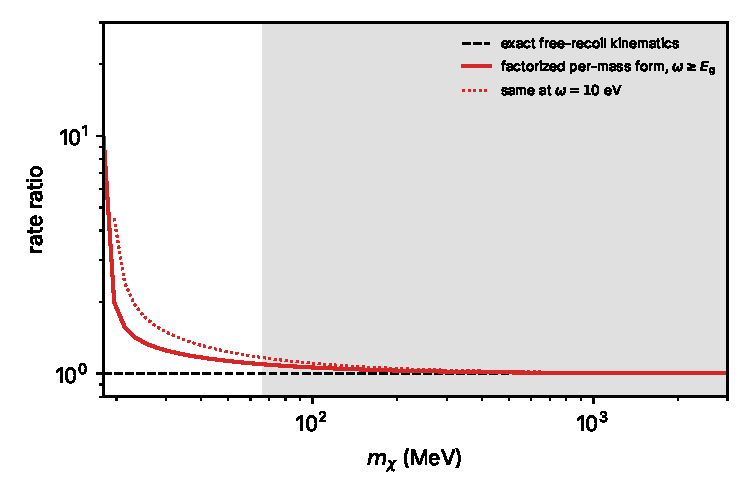
\includegraphics[width=\linewidth]{figures/ch12/limit12_3c.pdf}
\captionof{figure}{Migdal rate of silicon from the per-mass form \cref{eq:12.3-permass}, divided by the rate \cref{eq:12.3-rate} with the exact free-recoil kinematics, against the dark-matter mass. Solid: total rate for $\omega_e \ge \SI{1.11}{eV}$; dotted: the spectrum at $\omega_e = \SI{10}{eV}$. Both rates: heavy mediator, $\sigma_p = 10^{-38}\,\mathrm{cm}^2$, halo of \cref{sec:1.2}, the loss function with local fields and $Z_{\mathrm{ion}}(p)$, and momentum transfers above the impulse onset $q \ge \SI{92.5}{keV}$. Gray band: $\mchi \ge \SI{66}{MeV}$, where the total is within \SI{10}{\percent}.}\label{fig:12-limit-3c}
\par}
\smallskip
Below about \SI{60}{MeV} the electronic energy is no longer small against the kinetic energy of the dark matter. The per-mass form then overestimates the rate, by a factor 1.25 at \SI{30}{MeV} and 1.85 at \SI{20}{MeV}, and the exact $\vmin$ of \cref{eq:12.3-rate} must be kept.
\end{limitbox}

For orientation, at $\sigma_p = 10^{-38}\,\mathrm{cm}^2$ the exact rate \cref{eq:12.3-rate} above the onset is 1.9 events per kg and year at \SI{30}{MeV}, 30 at \SI{100}{MeV} and 970 at \SI{1}{GeV}. These are rates of primary pairs of a few eV, with the spectrum of \cref{fig:12-crystal-atom}. The number of electrons a detector counts follows from the cascade of \cref{chap:18}.

\section{Phonon final states at small momentum}\label{sec:12.4}

A dark-matter particle of \SI{2}{MeV} can transfer a momentum of at most $q = 2\mchi v_{\mathrm{max}} = \SI{10.6}{keV}$. At $q = \SI{10}{keV}$ a silicon nucleus would recoil with $E_R = \SI{1.9}{meV}$, less than the energy of most phonons, and the Debye--Waller exponent is $2W_\kappa = 0.063$: in \SI{94}{\percent} of the kicks the lattice is left exactly as it was (\cref{sec:11.3}). Yet the particle carries enough kinetic energy, $\frac12\mchi v_{\mathrm{max}}^2 = \SI{7}{eV}$, to make an electron--hole pair. If the electrons do not follow the kicked nucleus, a pair is made while the lattice stays in its ground state, and the whole deposit is electronic. The free recoil of \cref{sec:12.3} is the wrong lattice factor here; the impulse regime of \cref{sec:11.4} begins only at \SI{92.5}{keV}, that is at $\mchi = \SI{17.5}{MeV}$. Below it the lattice factor of the Migdal entry is the multiphonon response of \cref{sec:11.3} (\cref{sec:12.1-counting}).

Does the leading entry \cref{eq:12.1-Skk}, derived with a nucleus that is free during the electronic time, hold for a bound nucleus, and with the momentum $p$ taken by the electrons as large as the kick itself? It does, to a few parts in $10^3$ (\cref{sec:12.4-amp}). The real question at small $q$ is how a Migdal event shares its energy between electrons and lattice when the lattice can take zero, one or a few phonons.

\subsection{The amplitude of a bound nucleus}\label{sec:12.4-amp}

Write the Migdal process as two perturbations acting in turn: the kick $\ee^{\ii\vect{q}\cdot\vect{X}_I}$ from the dark matter, and the potential of nucleus $I$ acting on the electrons. By \cref{app:D.33-amp}, that potential is a sum of Fourier components $v_\kappa(\vect{p})\,\ee^{-\ii\vect{p}\cdot\vect{X}_I}\,n_e(\vect{p})$, and the electronic factor $v_\kappa(\vect{p})\langle\Psi_j|n_e(\vect{p})|\Psi_0\rangle$ is common to every term below. What depends on the lattice is the nuclear factor. Let $H_N$ be the Hamiltonian of the nuclei on the ground surface, with eigenstates $|\lambda\rangle$ of energy $E_\lambda$, the initial one $|0\rangle$. The two orderings of \cref{eq:2.4-orderings} give, for a final lattice state $f$ and electronic energy $\omega_e$,
\begin{equation}
  \mathcal{A}_f(\vect{q},\vect{p}) = \sum_\lambda\left[\frac{\langle f|\ee^{-\ii\vect{p}\cdot\vect{X}_I}|\lambda\rangle\langle\lambda|\ee^{\ii\vect{q}\cdot\vect{X}_I}|0\rangle}{\omega_e + E_f - E_\lambda}
  - \frac{\langle f|\ee^{\ii\vect{q}\cdot\vect{X}_I}|\lambda\rangle\langle\lambda|\ee^{-\ii\vect{p}\cdot\vect{X}_I}|0\rangle}{\omega_e + E_\lambda - E_0}\right] .
  \label{eq:12.4-exact}
\end{equation}
In the first ordering the kick acts first and the nucleus then passes $\vect{p}$ to the electrons; the denominator is the energy of the final state minus that of the intermediate one. In the second the electrons are excited first, by the nucleus at rest, and the intermediate state carries $\omega_e$ in addition to the lattice energy. This is the amplitude of Berghaus and collaborators~\cite[Eq.~(3.1)]{berghaus2023migdal}, with their lattice states as the $|\lambda\rangle$.

The electronic energy is large against the lattice energies that the matrix elements allow, and the denominators can be expanded in powers of $1/\omega_e$. Call $A = \ee^{-\ii\vect{p}\cdot\vect{X}_I}$ and $B = \ee^{\ii\vect{q}\cdot\vect{X}_I}$. Since $\langle f|H_N = E_f\langle f|$ and $H_N|0\rangle = E_0|0\rangle$, each power of $(E_f - E_\lambda)$ in the first term turns into a commutator with $H_N$ acting on $A$ from the left, and each power of $(E_\lambda - E_0)$ in the second into the same commutator acting on $A$ from the right. Order by order,
\begin{equation}
  \mathcal{A}_f = \frac{\langle f|[A,B]|0\rangle}{\omega_e} + \frac{\langle f|[[A,H_N],B]|0\rangle}{\omega_e^2} + \frac{\langle f|[[[A,H_N],H_N],B]|0\rangle}{\omega_e^3} + \cdots .
  \label{eq:12.4-series}
\end{equation}
The first term vanishes, since $A$ and $B$ are functions of the same position. For the second, $H_N = \sum_I\vect{P}_I^2/2M_\kappa + U(\{\vect{X}\})$ with any interatomic potential $U$. The potential commutes with $A$; the kinetic energy does not, because $A$ shifts the momentum of nucleus $I$ by $-\vect{p}$, $A\vect{P}_IA^\dagger = \vect{P}_I + \vect{p}$. Hence
\begin{equation*}
  [A,H_N] = \Bigl(\frac{\vect{p}\cdot\vect{P}_I}{M_\kappa} + \frac{p^2}{2M_\kappa}\Bigr)A , \qquad
  [[A,H_N],B] = \frac{\vect{p}}{M_\kappa}\cdot[\vect{P}_I,B]\,A = \frac{\vect{q}\cdot\vect{p}}{M_\kappa}\,\ee^{\ii(\vect{q}-\vect{p})\cdot\vect{X}_I} ,
\end{equation*}
and the leading nuclear factor is
\begin{equation}
  \mathcal{A}^{(2)}_f = \frac{\vect{q}\cdot\vect{p}}{M_\kappa\,\omega_e^2}\,\bigl\langle f\big|\ee^{\ii(\vect{q}-\vect{p})\cdot\vect{X}_I}\big|0\bigr\rangle .
  \label{eq:12.4-lead}
\end{equation}
This is the nuclear factor of \cref{eq:12.1-amp}, now obtained without any assumption about the binding of the nucleus. The interatomic potential has dropped out, as Berghaus and collaborators showed with their effective Hamiltonian $\nabla_IH_{\chi L}\cdot\nabla_IH_{eL}/(m_N\omega^2)$~\cite[Eq.~(3.6)]{berghaus2023migdal}. Esposito and Rocchi obtained the same matrix element from the first nonadiabatic correction to the Born--Oppenheimer product state~\cite[Eq.~(21)]{esposito2025migdal}, and showed that in an infinite crystal, whose center of mass does not move, the adiabatic part of the amplitude vanishes. Two routes therefore give one result: the boost of \cref{sec:8.6} and the second-order amplitude with the lattice integrated out.

The lattice enters at the next order, and the expansion shows what controls it. With $X = \vect{p}\cdot\vect{P}_I/M_\kappa + p^2/2M_\kappa$, the same steps give $[[[A,H_N],H_N],B] = (\vect{q}\cdot\vect{p}/M_\kappa)(2X - \vect{q}\cdot\vect{p}/M_\kappa)\,BA$, plus a term $-\ii(\vect{p}\cdot\nabla_IU/M_\kappa)A$ that commutes with $B$ and drops out. The potential first appears at order $\omega_e^{-4}$, through $[\vect{p}\cdot\nabla_IU,\vect{P}_I]$, the force constants. Summing $|\mathcal{A}_f|^2$ over all final states, averaging over the direction of $\vect{p}$ with the weight $(\vect{q}\cdot\vect{p})^2$ of the leading term, and collecting the terms of the first two orders,
\begin{equation}
  \frac{\sum_f|\mathcal{A}_f|^2}{\sum_f|\mathcal{A}^{(2)}_f|^2} = 1 - \frac{2p^2}{M_\kappa\,\omega_e} + \frac{2\langle\omega_{\mathrm{ph}}^2\rangle}{\omega_e^2} + \frac95\,\frac{v_N^2p^2}{\omega_e^2} + \cdots ,
  \label{eq:12.4-corr}
\end{equation}
with $v_N = q/M_\kappa$ and $\langle\omega_{\mathrm{ph}}^2\rangle$ the mean square phonon frequency seen by the nucleus. The first correction is the recoil energy of the momentum given to the electrons, $p^2/2M_\kappa$, over $\omega_e$: the expectation value of $2X - \vect{q}\cdot\vect{p}/M_\kappa$ in the kicked state is $\vect{p}\cdot(\vect{q} - \vect{p})/M_\kappa$, whose part odd in $\vect{p}$ averages away. The second is the binding of the nucleus, the factor $[1 - (\omega_{\mathrm{ph}}/\omega_e)^2]^{-2}$ that \cref{sec:6.1} found for a nucleus kicked in a harmonic well, at its first order. The third is the Doppler shift of the electronic energy by the moving nucleus, $\vect{v}_N\cdot\vect{p}$, at second order: for a free nucleus, \cref{eq:12.4-exact} is the bracket \cref{eq:12.3-bracket} with $b = \vect{q}\cdot\vect{p}/M_\kappa$, whose expansion $(b/\omega_e^2)(1 + b/\omega_e + b^2/\omega_e^2 + \cdots)$ squared and averaged with $\langle c^4\rangle/\langle c^2\rangle = 3/5$ gives the coefficient $9/5$.

None of the three is a ratio $p/q$, so the leading factor \cref{eq:12.4-lead} holds when the electrons take as much momentum as the nucleus receives, or more, as for the free nucleus of \cref{eq:12.3-bracket}. For silicon at $p = \SI{5.7}{keV}$, the median momentum of the Migdal weight (\cref{sec:12.3}), and $\omega_e = \SI{1.2}{eV}$, near the gap, the three terms of \cref{eq:12.4-corr} are $-2.1\times10^{-3}$, $+2.8\times10^{-3}$ (with the silicon phonon spectrum) and at most $5.1\times10^{-4}$ for every $q$ up to the impulse onset. The leading factor is exact to a few parts in $10^3$ throughout the region of this section. \Cref{lim:12.4a} below compares it with the full sum.

\subsection{Migdal rate with phonon final states}\label{sec:12.4-rate}

Squaring \cref{eq:12.4-lead}, summing over the nuclei and keeping the diagonal $\vect{G} = \vect{G}'$ of the electronic response and the self part of the lattice factor gives the Migdal entry with the lattice factor of one nucleus at the momentum $\vect{q} - \vect{p}$ that it keeps. For one nucleus per site the self response is $S^{\mathrm{ad}}_{\kappa;\vect{G}\vect{G}}(\vect{q} - \vect{k},\omega_l) = 2\pi\nd_\kappa\,s^{\mathrm{inc}}_\kappa(\vect{q} - \vect{k} - \vect{G},\omega_l)$, with $s^{\mathrm{inc}}_\kappa(\vect{Q},\omega)$ the spectrum of one nucleus normalized to $\int\dd\omega\,s^{\mathrm{inc}}_\kappa = 1$, zero-phonon line included. The self part is exact for the phonon-emitting terms, which are incoherent, and, averaged over the zone, for the zero-phonon term at $q \gtrsim 2q_{\mathrm{BZ}}$. Below the impulse onset that factor is the harmonic self response of \cref{eq:11.3-inc}, a zero-phonon line of weight $\ee^{-2W_\kappa}$ and the $n$-phonon spectra $P^\kappa_n$ with the Poisson weights \cref{eq:5.6-poisson}.
\begin{keyresult}[The Migdal probability with phonon final states]
At $n_B = 2$, for the valence electrons with the frozen-core vertex $v_\kappa = -Z_{\mathrm{ion}}(p)e^2/p^2$ of \cref{eq:12.3-Zion} and the diagonal loss function, a kick $\vect{q}$ of a nucleus of species $\kappa$ at a cubic site of a harmonic crystal at $T = 0$, with the incoherent lattice factor, leaves electronic energy $\omega_e$ and lattice energy $\omega_l$ with the probability density
\begin{equation}
  \begin{split}
  \frac{\dd^2P_{\mathrm{Mig}}}{\dd\omega_l\,\dd\omega_e} = 4\alpha\int\frac{\dd^3p}{(2\pi)^3}\;&Z_{\mathrm{ion}}(p)^2\,\frac{(\vect{v}_N\cdot\vect{p})^2}{\omega_e^4\,p^2}\,L(\vect{p},\omega_e)\,\ee^{-2W_\kappa(\vect{q}-\vect{p})} \\
  &\times\Biggl[\underbrace{\delta(\omega_l)}_{\text{zero-phonon, }\mathcal{P}_0} + \underbrace{\sum_{n\ge1}\frac{[2W_\kappa(\vect{q}-\vect{p})]^n}{n!}\,P^\kappa_n(\omega_l)}_{\text{phonon-emitting, }\mathcal{P}_+}\Biggr] .
  \end{split}
  \label{eq:12.4-harm}
\end{equation}
Integrated over $\omega_l$, the bracket times $\ee^{-2W_\kappa}$ gives one for every $\vect{p}$, and $\dd P_{\mathrm{Mig}}/\dd\omega_e$ is \cref{eq:12.3-soft} at every $q$ in this incoherent lattice form. The coherent zero-phonon process of the whole lattice has the same electronic spectrum, averaged over directions, for $q \gtrsim 2q_{\mathrm{BZ}}$. For $q \ll q_{\mathrm{BZ}}$ \cref{eq:8.3-boostward} fixes it at $(m_e/M_\kappa)^2(2q^2/e^2)L(\vect{q},\omega_e)/(2\pi\nd_\kappa)$, with $L$ the head of $-\varepsilon^{-1}$: in silicon $1/14.9$ of \cref{eq:12.3-soft}, with median $\omega_e = \SI{17.4}{eV}$ at the plasmon against \SI{4.5}{eV}. Between the two the coherent response is not computed (\cref{tab:12-nuisances}).
\end{keyresult}
\noindent This is the rate formula of Berghaus and collaborators~\cite[Eq.~(3.8)]{berghaus2023migdal}, with their partial structure factor in the incoherent harmonic form~\cite[Eqs.~(4.1), (4.5)]{berghaus2023migdal} and their effective charge $Z(k)$ as $Z_{\mathrm{ion}}$. Their full structure factor $S(\vect{q} - \vect{k}_e - \vect{K}, E)$ is the electron-following response of \cref{eq:12.1-Skk} at the momentum the nucleus keeps.

The sum rule in the key result, which Berghaus and collaborators pointed out, says that the electronic spectrum does not depend on the lattice dynamics. It needs no soft limit, since the lattice factor has unit weight at every $\vect{q} - \vect{p}$, and no impulse approximation. The lattice enters the rate only through energy conservation. In the double rate the lattice factor replaces the free recoil of \cref{eq:12.3-rate}. The weight $\dd E_R = q\,\dd q/M_\kappa$ is unchanged, and the minimum speed becomes $\vmin = (\omega_e + \omega_l)/q + q/2\mchi$, so that for a heavy mediator
\begin{equation}
  \frac{\dd^2\mathcal{R}}{\dd\omega_l\,\dd\omega_e} = \frac{\rho_\chi\,\sigma_N}{2\mchi\,\mu_{\chi N}^2M_\kappa}\int\dd q\;q\,\eta\Bigl(\frac{\omega_e + \omega_l}{q} + \frac{q}{2\mchi}\Bigr)\frac{\dd^2P_{\mathrm{Mig}}}{\dd\omega_l\,\dd\omega_e} .
  \label{eq:12.4-rate}
\end{equation}
Since $\omega_l$ is a few meV against an $\omega_e$ of a few eV, $\dd\mathcal{R}/\dd\omega_e$ hardly depends on how the lattice takes its share: replacing the free recoil by the bound response leaves the silicon rate unchanged (\cref{lim:12.3b}). What the lattice factor decides is the second axis of the joint response, the energy that a phonon sensor sees together with the charge. Berghaus, Essig and McDuffie extended \cref{eq:12.4-rate} to the nonrelativistic effective operators of the dark-matter--nucleon interaction~\cite{berghaus2026migdal}. Each operator multiplies the same electronic and lattice factors by its own nuclear response, and the lattice factor is again read at the momentum $\vect{q} - \vect{p}$ that the nucleus keeps.

\begin{limitbox}[Migdal effect with phonon final states][lim:12.4a]
$\dd^2P/\dd\omega_l\,\dd\omega_e = 4\alpha\int\dd^3p/(2\pi)^3\,Z_{\mathrm{ion}}(p)^2(\vect{v}_N\cdot\vect{p})^2L(\vect{p},\omega_e)\,s^{\mathrm{inc}}_\kappa(\vect{q} - \vect{p},\omega_l)/(\omega_e^4p^2)$, from the effective interaction $\nabla H_{\chi L}\cdot\nabla H_{eL}/(M_\kappa\omega_e^2)$~\cite[Eqs.~(3.6), (3.8)]{berghaus2023migdal}.
\par\smallskip
{\centering
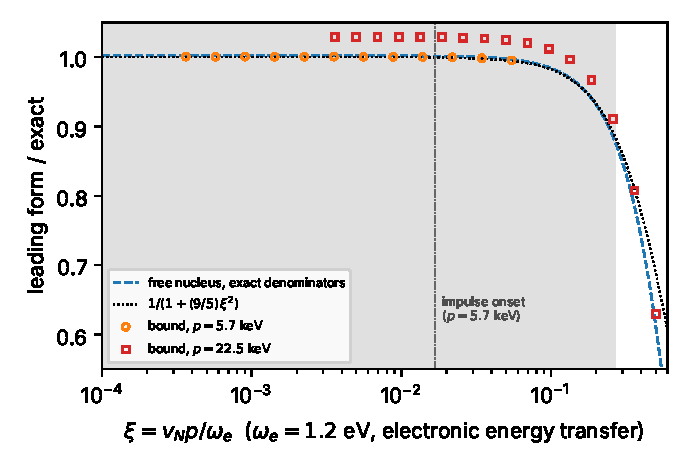
\includegraphics[width=\linewidth]{figures/ch12/limit12_4a.pdf}
\captionof{figure}{Migdal probability summed over all lattice final states, from the leading factor \cref{eq:12.4-lead}, divided by the same from the two time orderings \cref{eq:12.4-exact} with exact energy denominators, against $v_Np/\omega_e$ at the electronic energy transfer $\omega_e = \SI{1.2}{eV}$. Model: a silicon nucleus in an isotropic harmonic well of frequency $\omega_0 = \langle\omega^{-1}\rangle^{-1} = \SI{30.4}{meV}$, which has the Debye--Waller factor of the full phonon spectrum; direction of $\vect{p}$ averaged. Circles, $p = \SI{5.7}{keV}$ for $q = 2$ to \SI{300}{keV}; squares, $p = \SI{22.5}{keV}$ for $q$ up to \SI{700}{keV}, whose offset of 0.03 at small $v_Np/\omega_e$ is the recoil term $2p^2/M_\kappa\omega_e$. Dashed: free nucleus with exact denominators. Dotted: the leading correction $1/(1 + \frac95v_N^2p^2/\omega_e^2)$. Dash-dotted: the impulse onset at $p = \SI{5.7}{keV}$. Gray: within \SI{10}{\percent}, $v_Np/\omega_e \le 0.27$.}\label{fig:12-limit-4a}
\par}
\smallskip
The form fails when the Doppler shift $\vect{v}_N\cdot\vect{p}$ approaches $\omega_e$, at $q \approx \SI{1.5}{MeV}$ for $p = \SI{5.7}{keV}$ near the gap, far above the small-momentum region, where it holds to \num{e-3}.
\end{limitbox}

\noindent On the truncation label \cref{lim:12.4a} sits at $n_B = 2$, with $\mathfrak{M}$ = sudden, $\mathcal{K}$ = multiphonon at all orders (harmonic, incoherent), and $\mathcal{X}$ = random-phase with local fields on the diagonal. The diagonal is the approximation that costs most (\cref{sec:12.3-validity}).

\subsection{Zero-phonon, few-phonon and impulse regimes}\label{sec:12.4-regimes}

\Cref{fig:12-regimes} evaluates \cref{eq:12.4-harm} for silicon and sorts the Migdal events by the number of phonons they leave. The zero-phonon weight of the kick, $\ee^{-2W_\kappa(q)}$, falls to one half at $q = \SI{33.2}{keV}$, reached from $\mchi = \SI{6.3}{MeV}$. The impulse onset lies at \SI{92.5}{keV}. Below the first, most Migdal events are zero-phonon: at $q = \SI{10}{keV}$, \SI{92}{\percent} of them leave the lattice in its ground state, \SI{7.6}{\percent} emit one phonon and \SI{0.5}{\percent} two. Between the two boundaries a Migdal event emits a few phonons; at \SI{50}{keV} the fractions for zero, one, two and three or more are 0.21, 0.32, 0.25 and 0.22. Above the onset the lattice factor is the impulse Gaussian, and the soft-limit treatment of \cref{sec:12.3} holds.

\begin{figure}[tbp]
  \centering
  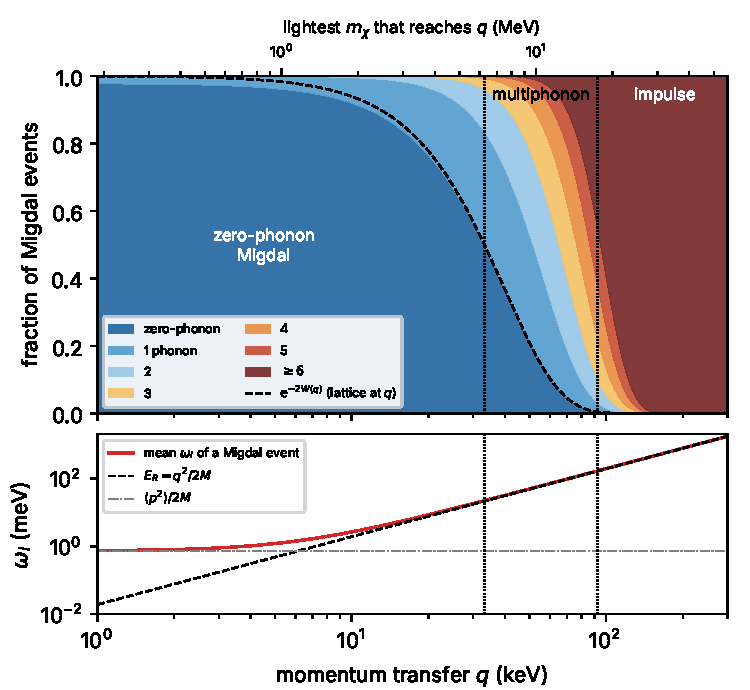
\includegraphics[width=0.84\linewidth]{figures/ch12/fig12_4.pdf}
  \caption{The three regimes of the Migdal effect in silicon against the momentum transfer $q$, at $T = 0$. Top: fraction of Migdal events that leave the lattice with zero, one, two, \ldots\ phonons, from \cref{eq:12.4-harm}, with the lattice factor at the momentum $\vect{q} - \vect{p}$ that the nucleus keeps, averaged over the momentum $\vect{p}$ given to the electrons with the weight $(\vect{q}\cdot\vect{p})^2Z_{\mathrm{ion}}(p)^2p^{-2}\int_{\Eg}\dd\omega_e\,L(p,\omega_e)/\omega_e^4$. Dashed: the zero-phonon weight $\ee^{-2W(q)}$ of the kick alone. Bottom: mean energy $\omega_l$ given to the lattice in a Migdal event, against the recoil energy $E_R$ and the recoil energy $\langle p^2\rangle/2M = \SI{0.72}{meV}$ of the electrons' momentum. Dotted lines: $\ee^{-2W(q)} = \frac12$ at \SI{33.2}{keV} and the impulse onset at \SI{92.5}{keV}. Top axis: the lightest dark matter that reaches $q$, $q/2v_{\mathrm{max}}$. Model: diagonal loss function with local fields of Knapen, Kozaczuk and Lin~\cite{knapen2021dark} (threshold \SI{1.11}{eV}, the step-model gap that accompanies the tables, $p \le \SI{22.5}{keV}$), $Z_{\mathrm{ion}}(p)$ of \cref{eq:12.3-Zion}, incoherent harmonic lattice factor with Poisson weights in $2W(Q) = Q^2\langle u_x^2\rangle$ from the PBE phonon spectrum of \cref{sec:5.2}.}
  \label{fig:12-regimes}
\end{figure}

At small $q$ the electrons' momentum controls the lattice. The momentum $p$ that the electrons take has $\langle p^2\rangle^{1/2} = \SI{6.1}{keV}$ in the weight of \cref{eq:12.4-harm}, and the nucleus keeps $\vect{q} - \vect{p}$, with $\langle|\vect{q} - \vect{p}|^2\rangle = q^2 + \langle p^2\rangle$. At \SI{5}{keV} this is 2.5 times $q^2$. The mean lattice energy of a Migdal event, $\langle|\vect{q} - \vect{p}|^2\rangle/2M_\kappa$ by the first moment of \cref{sec:11.3}, is then \SI{1.20}{meV}, 2.5 times the recoil energy, and at \SI{2}{keV} it is ten times $E_R$. The phonon-emitting fraction follows $2W_\kappa(\vect{q} - \vect{p})$, not $2W_\kappa(\vect{q})$: \SI{3.8}{\percent} at \SI{5}{keV}, against $1 - \ee^{-2W(q)} = \SI{1.6}{\percent}$. Above \SI{30}{keV} the difference fades, and at \SI{50}{keV} the mean lattice energy, \SI{48.5}{meV}, exceeds $E_R$ by \SI{1.5}{\percent}.

In the exact harmonic lattice factor, its part at $\omega_l = 0$ is the product of two ground-state expectation values of $n_\kappa$, which vanish unless $\vect{q} - \vect{p}$ is a reciprocal-lattice vector. A zero-phonon Migdal event is a Bragg process: the crystal takes a reciprocal-lattice vector $\vect{G}$ as a whole, with weight $\ee^{-2W_\kappa(\vect{G})}$ and the structure factor of the cell, and the electrons take exactly $\vect{p} = \vect{q} - \vect{G}$. The incoherent form in \cref{eq:12.4-harm} replaces this sum over discrete momenta by an integral over $\vect{p}$, which is its average over the zone (\cref{sec:11.3}). The two agree when the electronic weight varies slowly over $q_{\mathrm{BZ}}$. For silicon, averaging over the direction of $\vect{q}$ and keeping the diamond structure factor $|1 + \ee^{\ii\vect{G}\cdot\vect{\tau}}|^2$, the Bragg sum is 1.08, 1.04 and 1.03 times the incoherent integral at $q = 1.5$, 3 and \SI{5}{keV}, and within \SI{1}{\percent} of it from \SI{10}{keV}. This check keeps the diagonal $\vect{G} = \vect{G}'$ and averages over directions; the cross-site terms $\vect{G} \neq \vect{G}'$ of the coherent sum, which carry the screening of \cref{eq:8.3-boostward} at $q \ll q_{\mathrm{BZ}}$, are not tested by it. The electronic weight is spread over several zones, median $p = 2.5\,q_{\mathrm{BZ}}$, and the coherent sum samples it densely enough. For a fixed direction of $\vect{q}$ in a crystal at rest the sum depends on the orientation, which a direction-averaged rate does not see.

Germanium follows the same pattern at shifted boundaries. It has no first-principles phonon spectrum in this book (\cref{tab:5-phonons}). An estimate from its Debye temperature of \SI{373}{K}, scaled by the ratio 0.82 of the computed to the Debye value of $\langle\omega^{-1}\rangle^{-1}$ in silicon, gives $\langle\omega^{-1}\rangle^{-1} \approx \SI{17.6}{meV}$, and $\ee^{-2W(q)} = \frac12$ at $q \approx \SI{41}{keV}$, from $\mchi \approx \SI{7.7}{MeV}$. The impulse onset is at \SI{113}{keV}, from \SI{21.3}{MeV} (\cref{sec:11.4}). The heavier nucleus makes the recoil term of \cref{eq:12.4-corr} smaller by the mass ratio 2.6. The binding term is about the same as in silicon, $3\times10^{-3}$ at the germanium gap of \SI{0.67}{eV} with the phonon energies scaled by the ratio of the Debye temperatures.

\subsection{The phonon-mediated form}\label{sec:12.4-virtual}

Liang and collaborators describe the same process with the phonons as the intermediate states~\cite{liang2022phonon}. The kick creates on-shell phonons through the multiphonon vertex; one further phonon, virtual, carries momentum from the kicked nucleus to the bare electron--phonon vertex and excites a pair of energy $\varepsilon_i - \varepsilon_j$~\cite[Eq.~(3.1)]{liang2022phonon}. The virtual phonon brings the propagator $1/[(\varepsilon_i - \varepsilon_j)^2 - \omega_{\vect{Q}\nu}^2]$, which is the bound-nucleus form of the boost denominator, \cref{eq:12.4-pm}. For gaps large against the phonon energies they reduce it to $1/(\varepsilon_i - \varepsilon_j)^2$~\cite[Eq.~(3.2)]{liang2022phonon}, and with the completeness of the polarization vectors the amplitude becomes the leading one, with the lattice factor at $\vect{q}$ instead of $\vect{q} - \vect{p}$.

This form is exact at first order in $\vect{p}$ for a harmonic lattice. Write the displacement of nucleus $I$ in normal modes, $\vect{u}_I = \sum_\nu(\vect{\ell}_\nu a_\nu + \vect{\ell}_\nu^*a_\nu^\dagger)$, with $|\vect{\ell}_\nu|^2 = 1/(2NM_\kappa\omega_\nu)$ and $\nu$ running over the wavevectors and branches. The kick $B = \ee^{\ii\vect{q}\cdot\vect{u}_I}$, up to a phase, displaces every mode, $a_\nu B = B(a_\nu + \beta_\nu)$ with $\beta_\nu = \ii\vect{q}\cdot\vect{\ell}_\nu^*$. At first order in $\vect{p}$, $A = 1 - \ii\vect{p}\cdot\vect{u}_I$; the 1 drops out of \cref{eq:12.4-exact} as the first term of \cref{eq:12.4-series} does. The operator $\vect{p}\cdot\vect{u}_I$ changes one occupation by one, so the intermediate state differs from $f$ (first ordering) or from $0$ (second ordering) by one quantum, and the denominators are $\omega_e \mp \omega_\nu$ and $\omega_e + \omega_\nu$. Moving $a_\nu$ and $a_\nu^\dagger$ through $B$ with the displacement rule, $a_\nu B = B(a_\nu + \beta_\nu)$ and $Ba_\nu^\dagger = (a_\nu^\dagger - \beta_\nu^*)B$, the terms in $\langle f|a_\nu^\dagger B|0\rangle$ cancel between the two orderings, and what is left is proportional to $\langle f|B|0\rangle$:
\begin{equation}
  \mathcal{A}_f = -\ii\sum_\nu\Bigl[\frac{(\vect{p}\cdot\vect{\ell}_\nu)\beta_\nu}{\omega_e - \omega_\nu} + \frac{(\vect{p}\cdot\vect{\ell}_\nu^*)\beta_\nu^*}{\omega_e + \omega_\nu}\Bigr]\langle f|B|0\rangle
  = \frac{1}{N}\sum_\nu\frac{(\vect{q}\cdot\vect{e}_{\kappa\nu})(\vect{p}\cdot\vect{e}_{\kappa\nu}^*)}{M_\kappa(\omega_e^2 - \omega_\nu^2)}\,\bigl\langle f\big|\ee^{\ii\vect{q}\cdot\vect{X}_I}\big|0\bigr\rangle ,
  \label{eq:12.4-pm}
\end{equation}
for real polarization vectors $\vect{e}_{\kappa\nu}$, with $\vect{\ell}_\nu = \vect{e}_{\kappa\nu}/(2NM_\kappa\omega_\nu)^{1/2}$. The propagator is exact for every final state $f$, at all orders in $q$: the multiphonon blob and the virtual phonon factorize. At a cubic site the polarization sum is isotropic, $N^{-1}\sum_\nu e^\alpha_{\kappa\nu}e^{\beta*}_{\kappa\nu}\,\delta(\omega - \omega_\nu) = \delta_{\alpha\beta}\,g_{\mathrm{ph},\kappa}(\omega)/3$, and the propagator becomes $(\vect{q}\cdot\vect{p}/M_\kappa)\int\dd\omega\,g_{\mathrm{ph},\kappa}(\omega)/[3(\omega_e^2 - \omega^2)]$.
\begin{keyresult}[The phonon-mediated Migdal probability]
At first order in $\vect{p}$, for a harmonic crystal at $T = 0$ and a cubic site, the leading probability \cref{eq:12.4-harm} becomes
\begin{equation}
  \begin{split}
  \frac{\dd^2P_{\mathrm{Mig}}}{\dd\omega_l\,\dd\omega_e} = 4\alpha\int\frac{\dd^3p}{(2\pi)^3}\;&Z_{\mathrm{ion}}(p)^2\,\frac{(\vect{v}_N\cdot\vect{p})^2}{p^2}\,\biggl[\int\dd\omega\,\frac{g_{\mathrm{ph},\kappa}(\omega)/3}{\omega_e^2 - \omega^2}\biggr]^2L(\vect{p},\omega_e)\,\ee^{-2W_\kappa(\vect{q})} \\
  &\times\Biggl[\underbrace{\delta(\omega_l)}_{\text{zero-phonon}} + \underbrace{\sum_{n\ge1}\frac{[2W_\kappa(\vect{q})]^n}{n!}\,P^\kappa_n(\omega_l)}_{\text{phonon-emitting}}\Biggr] ,
  \end{split}
  \label{eq:12.4-pmrate}
\end{equation}
with the lattice factor at the kick $\vect{q}$. For $\omega_e \gg \omega_{\mathrm{ph}}$ the squared bracket is $\omega_e^{-4}[1 + 2\langle\omega_{\mathrm{ph}}^2\rangle/\omega_e^2 + \cdots]$, with $\langle\omega_{\mathrm{ph}}^2\rangle$ the mean of $\omega^2$ over $g_{\mathrm{ph},\kappa}/3$.
\end{keyresult}
\noindent With the propagator reduced to $\omega_e^{-2}$ this is the rate of Liang and collaborators~\cite[Eqs.~(3.3), (3.4)]{liang2022phonon}, whose $T_0(E) = \delta(E)$ is the zero-phonon term and whose $T_n$ with $n \ge 1$ are the phonon-emitting terms. Their factor $\Imag[-\tilde\varepsilon^{-1}_{\vect{G}\vect{G}'}]$ keeps the elements $\vect{G} \neq \vect{G}'$ that \cref{eq:12.4-pmrate} drops, and their $Z_{\mathrm{ion}}$ is the constant valence charge.

The zero-phonon term dominates wherever the phonon-mediated form is needed. At $q = \SI{5}{keV}$ it holds \SI{96}{\percent} of the Migdal events, and a rate that kept only the phonon-emitting terms would be low by a factor 26. The first numerical evaluation of the phonon-mediated rate omitted $T_0$ and found rates far below the free-recoil ones at small mass; with $T_0$ restored the two agree at all masses~\cite[Note added]{liang2022phonon}, as the sum rule under \cref{eq:12.4-harm} requires.

The two published forms are complementary truncations of \cref{eq:12.4-exact}. The leading form \cref{eq:12.4-harm} is exact in $\vect{p}$ and keeps the first order in $1/\omega_e$; the phonon-mediated form \cref{eq:12.4-pmrate} is exact in $\omega_{\mathrm{ph}}/\omega_e$ and keeps the first order in $\vect{p}$. Their difference at order $p^2$ is the lattice factor at $\vect{q} - \vect{p}$ against $\vect{q}$. For the electronic spectrum it is immaterial, since both lattice factors have unit weight. For the lattice spectrum it is not: at \SI{5}{keV} the phonon-emitting fraction is \SI{3.8}{\percent} with the lattice factor at $\vect{q} - \vect{p}$ and \SI{1.6}{\percent} at $\vect{q}$, because the electrons' momentum is larger than the kick. In the frame of the crystal, where the transition density is frozen and the nucleus feels the recoil of $\vect{p}$, the all-orders form is the correct one. The exact sum over a harmonic site confirms it (\cref{we:12-five-keV}). The frame itself is the open question of \cref{sec:12.1-boost}.

\begin{limitbox}[Phonon-mediated Migdal effect][lim:12.4b]
$\dd^2P/\dd\omega_l\,\dd\omega_e$ as \cref{lim:12.4a} with the propagator $(\vect{q}\cdot\vect{p}/M_\kappa)\sum_\nu|\vect{e}_\nu|^2/[N(\omega_e^2 - \omega_\nu^2)]$ reduced to $\vect{q}\cdot\vect{p}/(M_\kappa\omega_e^2)$, the lattice factor at $\vect{q}$ and its zero-phonon term included~\cite[Eqs.~(3.1)--(3.4)]{liang2022phonon}.
\par\smallskip
{\centering
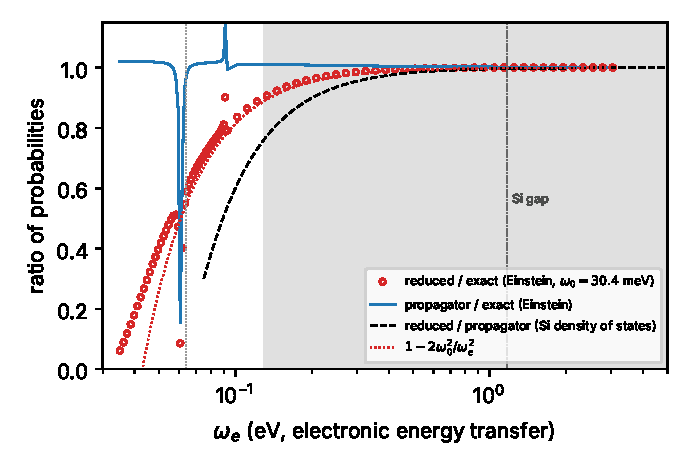
\includegraphics[width=\linewidth]{figures/ch12/limit12_4b.pdf}
\captionof{figure}{Migdal probability summed over lattice final states against the electronic energy transfer $\omega_e$, at $q = \SI{10}{keV}$ and $p = \SI{5.7}{keV}$, direction of $\vect{p}$ averaged. Circles: the reduced form over the exact second-order amplitude \cref{eq:12.4-exact} of a silicon nucleus in an isotropic harmonic well of frequency $\omega_0 = \SI{30.4}{meV}$. Solid: the unreduced propagator form \cref{eq:12.4-pm} over the same exact result; its narrow feature at $\omega_e = 2\omega_0$ is the two-phonon intermediate state, of relative weight $p^2/(2M_\kappa\omega_0) = 0.02$, which the first-order form lacks. Dotted: the leading correction $1 - 2\omega_0^2/\omega_e^2$. Dashed: reduced over propagator form with the PBE phonon spectrum of silicon (PBE band top \SI{63.7}{meV}, dotted vertical line). Gray: reduced form within \SI{10}{\percent} of the exact one, $\omega_e \ge 4.2\,\omega_0$. Dash-dotted: the silicon gap.}\label{fig:12-limit-4b}
\par}
\smallskip
The reduced form fails where $\omega_e$ approaches the phonon band, below \SI{0.20}{eV} with the silicon spectrum, where the electrons no longer see a sudden kick and the pole at $\omega_e = \omega_\nu$ turns the process into the absorption of a real phonon.
\end{limitbox}

\noindent On the truncation label \cref{lim:12.4b} sits at $n_B = 2$, with $\mathfrak{M}$ = sudden and the bound denominators $\omega_e^2 - \omega_\nu^2$, $\mathcal{K}$ = multiphonon at all orders with the lattice factor at $\vect{q}$, and $\mathcal{X}$ = random-phase with local fields. Its leading correction is one step of $n_B$, from 2 to 4: the phonon energies in the electronic denominators, of relative size $2\langle\omega_{\mathrm{ph}}^2\rangle/\omega_e^2$, as \cref{sec:8.5} counts it.

Silicon and germanium do not need the propagator. At the silicon gap of \SI{1.17}{eV} the reduced form is low by \num{2.9e-3}, at the germanium gap by about \num{3e-3}, and averaged over the silicon spectrum by \num{3e-4}. It is needed where the gap is comparable with the phonon energies: the narrow-gap and Dirac materials of \cref{chap:16}, whose gaps of tens of meV were the motivation of the phonon-mediated description, and the metals of \cref{sec:12.1-gapless}. There the region $\omega_e \lesssim 3\omega_{\mathrm{ph}}$ is not a Migdal process with a small correction but the electron--phonon response of the target.

\begin{workedexample}{The phonon-mediated term at $q = \SI{5}{keV}$}\label{we:12-five-keV}
A silicon nucleus kicked with $q = \SI{5}{keV}$ recoils with $E_R = q^2/2M_\kappa = \SI{0.478}{meV}$ and velocity $v_N = 1.91\times10^{-7}$, \SI{57}{m/s}. The momentum is reached by dark matter of $\mchi \ge q/2v_{\mathrm{max}} = \SI{0.94}{MeV}$; at \SI{1}{MeV} the largest energy transfer at this $q$, $qv_{\mathrm{max}} - q^2/2\mchi$, is \SI{0.75}{eV}, below the gap, and at \SI{2}{MeV} it is \SI{7.0}{eV}. The Debye--Waller exponent is $2W_\kappa(q) = 0.0157$. The momentum is 2.2 times $q_{\mathrm{BZ}}$, below the 2.95\,$q_{\mathrm{BZ}}$ from which \cref{sec:11.3} shows the incoherent multiphonon terms to hold and the \SI{18}{keV} from which the incoherent one-phonon term holds.

\emph{The probability.} By the sum rule of \cref{eq:12.4-harm}, the electronic spectrum is \cref{eq:12.3-soft} with the recoil energy $E_R$. At $q = 2.2\,q_{\mathrm{BZ}}$ this is the direction-averaged coherent process, within the $\vect{G} \neq \vect{G}'$ row of \cref{tab:12-nuisances}. With $Z_{\mathrm{ion}}(p)$, local fields and $\omega_e \ge \SI{1.11}{eV}$, \cref{sec:12.3} gives $6.07\times10^{-5}$ per eV of recoil energy, so $P_{\mathrm{Mig}} = 2.90\times10^{-8}$. One kick in $3.4\times10^7$ makes a pair.

\emph{The propagator.} With the PBE phonon spectrum, $\langle\omega_{\mathrm{ph}}^2\rangle^{1/2} = \SI{44.7}{meV}$. The squared bracket of \cref{eq:12.4-pmrate} times $\omega_e^4$ is 1.0029 at \SI{1.17}{eV}, the leading correction $2\langle\omega_{\mathrm{ph}}^2\rangle/\omega_e^2 = \num{2.9e-3}$, and 1.0003 averaged over the electronic spectrum, half of which lies above \SI{4.6}{eV}. The virtual phonon is far off shell, and the bound-nucleus correction is negligible.

\emph{The zero-phonon term.} With the lattice factor at $\vect{q} - \vect{p}$, \SI{96.2}{\percent} of the Migdal events leave no phonon, $P = 2.79\times10^{-8}$: the crystal takes the momentum as a whole, and all of the deposit, a few eV, is electronic. With the lattice factor at $\vect{q}$, as in \cref{eq:12.4-pmrate}, the share is \SI{98.4}{\percent}.

\emph{The phonon-emitting terms.} The rest, $1.10\times10^{-9}$, emits one phonon in \SI{96}{\percent} of the cases. Its energy follows the one-phonon spectrum of the incoherent response, $g_{\mathrm{ph},\kappa}(\omega)/\omega$, with mean $\langle\omega^{-1}\rangle^{-1} = \SI{30.4}{meV}$ and median \SI{21.7}{meV}: a phonon-emitting Migdal event gives the lattice 64 times the recoil energy. The energy comes from the dark matter, not from the recoil: kinematics bounds only the sum $\omega_e + \omega_l$, by \SI{7.0}{eV} at \SI{2}{MeV}, and a phonon costs a small part of it. Averaged over all Migdal events, the lattice receives \SI{1.20}{meV}, 2.5 times $E_R$, almost all in the rare events with a phonon.

\emph{A check.} Take a nucleus in a harmonic well of frequency \SI{30.4}{meV}, with $p = \SI{5.7}{keV}$ and $\omega_e = \SI{1.2}{eV}$. The exact amplitude \cref{eq:12.4-exact}, summed over final states, is 0.99934 times the leading form \cref{eq:12.4-lead} and 0.9980 times the propagator form \cref{eq:12.4-pm}. Its zero-phonon fraction is 0.967, against 0.984 for the lattice factor at $\vect{q}$ alone.
\end{workedexample}

The frame of the transition density, the lattice factor at small $|\vect{q} - \vect{p}|$ and the off-diagonal electronic response remain open at small momentum. The frame is the Herzberg--Teller term of \cref{sec:12.1-boost}, and at \SI{5}{keV} it is the factor 2.4 between the phonon-emitting fractions above; the electronic spectrum does not depend on it. Below $|\vect{q} - \vect{p}| \approx \SI{6.6}{keV}$ the incoherent multiphonon terms are not certified (\cref{lim:11.3a}), while the zero-phonon line, the dominant term, agrees with its diagonal, direction-averaged Bragg sum within \SI{8}{\percent}. The elements $\vect{G} \neq \vect{G}'$ of the electronic response are common to all crystal forms (\cref{app:E.18}). The frame and the lattice factor change the lattice spectrum of Migdal events, not their number, and \cref{tab:12-nuisances} carries all three.

\section{Moments of the Migdal spectrum}\label{sec:12.5}

A silicon nucleus kicked to a recoil energy of \SI{500}{eV} leaves its valence electrons excited in three events out of a hundred and gives them on average \SI{0.18}{eV} per kick, \SI{0.28}{eV} with the core shells. The second number needs no excited state of the crystal. It is the recoil energy times the ratio of the drag mass, the mass of the electrons that a slowly moving nucleus carries with it, to the mass of the nucleus. Every moment of the Migdal spectrum is fixed in the same way by the force that the electrons exert on one nucleus. The moments give the size of the effect without a spectrum, test a computed spectrum, bound the Migdal probability from both sides, and fix how a Migdal rate is added to a lattice rate.

\subsection{Inverse moments of the force spectrum}\label{sec:12.5-moments}

The force of \cref{eq:12.1-force} has a spectrum. With $|0\rangle$ the ground state of the clamped electrons, $|a\rangle$ their excited states and $\Delta_a = E_a - E_0$, we define the spectral measure of its component along the kick and its inverse moments,
\begin{equation}
  \dd\sigma_\kappa(\Delta) = \sum_{a\neq0}\bigl|\hat{\vect{q}}\cdot\langle a|\nabla_{\vect{R}_\kappa}V_{eN}|0\rangle\bigr|^2\,\delta(\Delta - \Delta_a) , \qquad
  \mathcal{I}_k = \int\Delta^{-k}\,\dd\sigma_\kappa(\Delta) ,
  \label{eq:12.5-sigma}
\end{equation}
for one nucleus $\vect{R}_\kappa$ of species $\kappa$. The leading-order Migdal probability \cref{eq:8.6-PMig}, with $\vect{d}_{a0} = -\vect{F}_{a0}/\Delta_a$ from \cref{eq:5.1-dcoup}, resolved in the electronic energy, is
\begin{equation}
  \frac{\dd P_{\mathrm{Mig}}}{\dd\omega_e} = \frac{q^2}{M_\kappa^2\,\omega_e^4}\,\frac{\dd\sigma_\kappa}{\dd\Delta}\bigg|_{\Delta = \omega_e} .
  \label{eq:12.5-spectrum}
\end{equation}
It is the electronic marginal of the Migdal entry \cref{eq:12.1-Skk}, divided by $2\pi\nd_\kappa$, once the lattice factor has been integrated over $\omega_l$ with its unit weight.

\begin{keyresult}[Moments of the Migdal spectrum]
At leading order in the boost, for a nucleus of species $\kappa$ kicked with momentum $\vect{q}$ and $E_R = q^2/2M_\kappa$,
\begin{equation}
  \begin{gathered}
  \int\dd\omega_e\,\omega_e^k\,\frac{\dd P_{\mathrm{Mig}}}{\dd\omega_e} = \frac{q^2}{M_\kappa^2}\,\mathcal{I}_{4-k} : \\
  \underbrace{P_{\mathrm{Mig}} = \frac{q^2\mathcal{I}_4}{M_\kappa^2}}_{k = 0} , \quad
  \underbrace{E^{\mathrm{Mig}}_1 = E_R\,\frac{\delta M_\kappa}{M_\kappa}}_{k = 1,\ \delta M_\kappa = 2\mathcal{I}_3} , \quad
  \underbrace{E^{\mathrm{Mig}}_2 = \frac{q^2\mathcal{I}_2}{M_\kappa^2}}_{k = 2} , \quad
  \underbrace{E^{\mathrm{Mig}}_3 = \frac{q^2\mathcal{I}_1}{M_\kappa^2}}_{k = 3} ,
  \end{gathered}
  \label{eq:12.5-moments}
\end{equation}
with $E^{\mathrm{Mig}}_k$ the $k$th moment. The first moment is the Born--Huang drag mass of \cref{eq:8.6-fsum-k} along $\hat{\vect{q}}$, times $E_R/M_\kappa$.
\end{keyresult}
\noindent Every moment is proportional to $E_R$, so each defines a material constant per unit recoil energy. Each also has a meaning in the ground state of the clamped electrons. The first is the drag mass of Born and Huang~\cite[App.~VIII]{born1954dynamical}: $\delta M_\kappa = 2\mathcal{I}_3$ is \cref{eq:D.28-dM} projected on $\hat{\vect{q}}$, the identity that \cref{sec:12.1-boost} used to estimate $P_{\mathrm{Mig}}$. It is also the curvature in frequency of the electronic force constant. A nucleus displaced at frequency $\omega$ below the gap feels the force constant $\Phi^{\mathrm{el}}_{\kappa\kappa}(\omega) = \langle\partial^2_{\hat q}V_{eN}\rangle - 2\int\dd\sigma_\kappa(\Delta)\,\Delta/(\Delta^2 - \omega^2)$, whose expansion in $\omega^2$ is $\Phi^{\mathrm{el}}_{\kappa\kappa}(0) - \omega^2\delta M_\kappa + O(\omega^4)$. The equation of motion $[\Phi(\omega) - \omega^2M_\kappa]u = 0$ then moves with the mass $M_\kappa + \delta M_\kappa$: the electrons that follow a slow nucleus add their inertia to it. The second moment is the diagonal Born--Huang correction of \cref{app:D.28}, $E_{\mathrm{BH}} = \mathcal{I}_2/2M_\kappa$ along $\hat{\vect{q}}$, so that $E^{\mathrm{Mig}}_2 = 4E_RE_{\mathrm{BH}}$. The third is the second-order energy of the electrons in the field of a displaced nucleus, and \cref{sec:12.5-third} turns it into the electron density at the nucleus.

The force spectrum of the valence electrons follows from the loss function. Comparing \cref{eq:12.5-spectrum} with the soft-limit probability \cref{eq:12.3-soft} gives, for the diagonal $\vect{G} = \vect{G}'$ and the frozen-core vertex of \cref{eq:12.3-Zion},
\begin{equation}
  \begin{gathered}
  \frac{\dd\sigma_\kappa}{\dd\omega} = \frac{e^2}{\pi}\int\frac{\dd^3p}{(2\pi)^3}\;Z_{\mathrm{ion}}(p)^2\,\frac{(\hat{\vect{q}}\cdot\vect{p})^2}{p^2}\,L(\vect{p},\omega) , \\
  \delta M^{\mathrm{val}}_\kappa = \frac{8\alpha}{3}\int\frac{\dd^3p}{(2\pi)^3}\;Z_{\mathrm{ion}}(p)^2\int_0^\infty\frac{\dd\omega}{\omega^3}\,\bar L(p,\omega) ,
  \end{gathered}
  \label{eq:12.5-dMval}
\end{equation}
the second form for a direction-averaged loss function, with $e^2/\pi = 4\alpha$. The drag mass of the valence electrons is a property of the clamped crystal, like the static dielectric constant, which fixes the $\omega^{-1}$ moment of the same loss function at $p \to 0$ (\cref{sec:4.4}).

The inverse moments come from linear-response calculations without any excited state. The drag mass is the $\omega^2$ coefficient of the on-site force constant, which the frequency-dependent Sternheimer equation of \cref{app:E.4} returns at a few imaginary frequencies, where the sign of the $\omega^2$ term changes, $\Phi^{\mathrm{el}}_{\kappa\kappa}(\ii\omega) = \Phi^{\mathrm{el}}_{\kappa\kappa}(0) + \omega^2\delta M_\kappa + O(\omega^4)$. Two static Sternheimer solves per occupied state give $\mathcal{I}_2$, $\mathcal{I}_3$ and $\mathcal{I}_4$ at the level of independent pairs.

\subsection{On-site drag mass and trace rule}\label{sec:12.5-trace}

The drag mass of a rigid translation and the on-site drag mass of one nucleus must be kept apart. Displace every nucleus of a crystal by the same $\vect{u}$, slowly. The electrons see a rigidly translated potential and follow it exactly, so the whole crystal moves with the mass of nuclei and electrons together. Let $\delta M_{IJ}$ be the drag-mass tensor between nuclei $I$ and $J$, defined as in \cref{eq:D.28-dM} with the forces of the two nuclei. The translation then gives the \emph{trace rule}
\begin{equation}
  \sum_J\delta M_{IJ} = Z_\kappa m_e\,\mathbf{1} \quad\text{(one species)} , \qquad
  \sum_{\kappa\kappa'}\delta M_{\kappa\kappa'}(\vect{Q} = 0) = N_em_e\,\mathbf{1} \quad\text{per cell} ,
  \label{eq:12.5-trace}
\end{equation}
which follows from the f-sum rule of the electrons in velocity form, because the summed force $\sum_J\nabla_JV_{eN}$ is the time derivative of the total electronic momentum (\cref{app:D.34-trace}). It holds for any insulator and any interaction among the electrons. For a free atom there is only one nucleus, the sum has one term, and it is the Thomas--Reiche--Kuhn value $N_em_e$ of \cref{eq:8.6-fsum-k}. The estimate $14\,m_e$ that \cref{sec:8.6} took for silicon is this sum; it is exact, but a kick probes a different element.

A dark-matter particle kicks one nucleus. The Migdal moments \cref{eq:12.5-moments} contain the force of nucleus $I$ alone, and $\delta M_\kappa$ in them is the on-site element $\delta M_{II}$. Written in phonon wavevectors, $\delta M_{II}$ is the average over the Brillouin zone of $\delta M_{\kappa\kappa}(\vect{Q})$, while \cref{eq:12.5-trace} fixes only the value at $\vect{Q} = 0$. The two differ by the off-site coupling,
\begin{equation}
  \delta M_{II} = Z_\kappa m_e - \sum_{J\neq I}\delta M_{IJ} ,
  \label{eq:12.5-onsite}
\end{equation}
which no sum rule fixes, in size or in sign. Positivity of the tensor at each $\vect{Q}$ gives $\delta M_{II} \ge 0$ and nothing more.

Silicon shows what the two elements are. Its cores move rigidly with the nucleus and contribute their own count to every element. The atomic Migdal tables of Cox and collaborators~\cite{cox2023precise}, rescaled to dipole order as in \cref{sec:12.2}, confirm this. The first moments of the $1s$, $2s$ and $2p$ ionization spectra, with the measured binding energies, add up to $10.1\,m_e$, of which $7.2\,m_e$ is $2p$. The valence part depends on the crystal. Evaluated on the loss function of Knapen, Kozaczuk and Lin with local fields, the table of \cref{sec:12.3}, \cref{eq:12.5-dMval} gives $\delta M^{\mathrm{val}} = 18.6\,m_e$, and with the cores the on-site drag mass is $28.7\,m_e$, $\delta M_{II}/M = 5.60\times10^{-4}$, twice the trace value. In the free atom the four valence electrons carry $4\,m_e$ in all, of which their ionization spectra carry $1.2\,m_e$ and the bound transitions the rest.

In silicon \SI{96}{\percent} of the valence integral comes from $p > q_{\mathrm{BZ}}$ and \SI{61}{\percent} from $p > \SI{5}{keV}$, where the ion charge has risen from 4 to 4.84 and the probe resolves the core region. In energy, \SI{67}{\percent} lies below \SI{10}{eV}, near the gap, where the weight $\omega^{-3}$ is largest. The table stops at \SI{89}{eV}; the valence f-sum held by the table bounds the missing part at \SI{24}{\percent}. Momenta above \SI{10}{keV} carry \SI{2.8}{\percent} of the integral, so those beyond the table's \SI{22.5}{keV} are estimated to add less. The approximations matter more than the truncation. A point ion of charge 4 gives $11.8\,m_e$, and the loss function without local fields $24.0\,m_e$. Both are uncontrolled at $p \gtrsim \SI{5}{keV}$. The frozen-core vertex assumes that the valence electrons inside the core region feel the bare nucleus screened by a rigid core. The diagonal $\vect{G} = \vect{G}'$ drops the off-diagonal elements of the dielectric matrix, which are sized only in a model and only for the rate (\cref{sec:12.3-validity}); the local fields on the diagonal already move the valence drag mass from $24.0$ to $18.6\,m_e$.

The excess over the trace value has no sign fixed by anything above. A model shows that it can go either way. In a periodic chain of Gaussian wells, two independent electrons per well and one filled band (\cref{app:D.34-trace}), the trace rule \cref{eq:12.5-trace} holds to $10^{-4}$ for every depth of the wells. The on-site element equals $2\,m_e$ while the wells are deep and isolated, and falls to $1.29\,m_e$ at a gap of \SI{8.1}{eV} and to $0.92\,m_e$ at \SI{5.4}{eV} as they overlap: with short-range wells the neighbors take part of the drag, and $\sum_{J\neq I}\delta M_{IJ} > 0$. The silicon table gives the opposite sign, $\sum_{J\neq I}\delta M_{IJ} = -14.7\,m_e$, from the long-range Coulomb vertex at large $p$ that the chain lacks. No calculation of $\delta M_{\kappa\kappa}(\vect{Q})$ exists that could decide between the two pictures for silicon. We therefore take the on-site valence drag mass of silicon as $18.6\,m_e$, with the band $12$ to $24\,m_e$ from the vertex and the local fields, and carry the band in the uncertainty budget of the chapter (\cref{tab:12-nuisances}). For germanium the same tables give $39.5\,m_e$, with the band $11.5$ to $52\,m_e$: the frozen $3d$ shell is shallow, bound by only \SI{29.4}{eV} and extended to \SI{0.4}{\angstrom}, and $Z_{\mathrm{ion}}(p)$ climbs from 4 already at a few keV. The cores of germanium carry $26.8\,m_e$ in the atomic tables without the $1s$, close to the $26\,m_e$ of a rigid core without the $1s$.

The difference between the two elements also tells which mass the lattice responses of \cref{chap:11} should carry. An incoherent kick probes $\delta M_{II}$. A coherent phonon of wavevector $\vect{Q}$ probes $\delta M_{\kappa\kappa'}(\vect{Q})$, and a long-wavelength acoustic phonon, which translates the whole cell, carries exactly the full mass of the atoms, $M_\kappa + Z_\kappa m_e$. The prescription of \cref{sec:8.6} and \cref{sec:12.1-counting}, mass $M_\kappa + \delta M_\kappa$ in the electron-following response, uses the on-site element for the impulse and multiphonon responses of an incoherent kick.

\subsection{Bounds on the Migdal probability}\label{sec:12.5-bounds}

The first moment and the threshold bound the probability from above, and the first and second moments bound it from below. On the support of the force spectrum every energy exceeds the threshold $E_{\mathrm{th}}$ of the electrons, the gap for the valence and the binding energy for a core shell, so $\mathcal{I}_4 \le \mathcal{I}_3/E_{\mathrm{th}}$. The Cauchy--Schwarz inequality for the measure $\dd\sigma_\kappa$, applied to the functions $\Delta^{-1}$ and $\Delta^{-2}$, gives $\mathcal{I}_3^2 \le \mathcal{I}_2\mathcal{I}_4$. With \cref{eq:12.5-moments} the two become a statement about the measured quantities.
\begin{keyresult}[Bounds on the Migdal probability]
For a nucleus kicked with recoil energy $E_R$, with the Migdal spectrum split into groups of final states $s$ (valence and core shells) with thresholds $E_s$ and drag masses $\delta M_s$, $\sum_s\delta M_s = \delta M_\kappa$,
\begin{equation}
  \frac{(E^{\mathrm{Mig}}_1)^2}{E^{\mathrm{Mig}}_2} \;\le\; P_{\mathrm{Mig}} \;\le\; \sum_s\frac{E_R}{E_s}\,\frac{\delta M_s}{M_\kappa} \;\le\; \frac{E_R}{\Eg}\,\frac{\delta M_\kappa}{M_\kappa} .
  \label{eq:12.5-bound}
\end{equation}
\end{keyresult}
\noindent The upper bound needs only the drag mass and the threshold, the two numbers a static calculation gives most reliably. It is reached when the whole force spectrum lies at the threshold, and the shell-resolved form is much tighter than the last one because the core shells, which hold a large part of $\delta M_\kappa$, have thresholds a hundred times the gap. The lower bound is reached when the spectrum is a single line. The ratio of the two bounds measures the width of the spectrum in energy.

On the silicon table the valence probability is \SI{19}{\percent} of its upper bound and 1.74 times its lower bound; for germanium the numbers are \SI{15}{\percent} and 1.92. The mean energy $E^{\mathrm{Mig}}_1/P_{\mathrm{Mig}}$ of the valence spectrum is \SI{6.0}{eV} in silicon and \SI{5.1}{eV} in germanium, five to seven times the gap, which is why the upper bound is loose. For the $2p$ shell of the silicon atom the probability is \SI{50}{\percent} of its bound, since a core spectrum begins with a sharp edge. The bounds carry the leading-order caveat of \cref{eq:12.5-moments}. At large recoil the motion of the nucleus during the transition, the free-recoil bracket \cref{eq:12.3-bracket}, raises the probability by the factor 1.6 at \SI{500}{eV} (\cref{sec:12.3-validity}); the bounds apply to the leading-order spectrum.

A lattice response added to a Migdal rate takes the weight $1 - P_{\mathrm{Mig}}$ of \cref{eq:12.1-zeroth}. On the silicon table the valence probability reaches $10^{-3}$ at $E_R = \SI{16.5}{eV}$ and grows linearly from there. The mass correction is smaller. It moves the mean of the impulse response by $-E_R\,\delta M_{II}/M_\kappa$, a few parts in $10^4$ of $E_R$, while the impulse width $E_Rx_R^{-1/2}$ of \cref{sec:11.4} is a percent of $E_R$ at these energies.

\begin{workedexample}{The silicon drag mass and the bound on the Migdal probability at \SI{500}{eV}}\label{we:12-drag}
A silicon nucleus, $M = \SI{26.16}{GeV}$, recoils with $E_R = \SI{500}{eV}$ when it receives $q = (2ME_R)^{1/2} = \SI{5.11}{MeV}$; its velocity is $v_N = 1.96\times10^{-4}$. The drag masses of \cref{sec:12.5-trace} are $10.1\,m_e$ for the cores and $18.6\,m_e$ for the valence, so $\delta M_{II} = 28.7\,m_e$ and $\delta M_{II}/M = 5.60\times10^{-4}$, against $2.73\times10^{-4}$ for the trace value $14\,m_e$. The first moment is $E^{\mathrm{Mig}}_1 = E_R\,\delta M_{II}/M = \SI{0.280}{eV}$: \SI{0.099}{eV} from the cores and \SI{0.181}{eV} from the valence.

The bounds follow shell by shell. The valence, with the threshold \SI{1.11}{eV} of the table, has $P \le 0.181/1.11 = 0.163$; its second moment, $E^{\mathrm{Mig}}_2 = \SI{1.89}{eV^2}$, gives $P \ge 0.181^2/1.89 = 0.0174$. The computed spectrum gives $P = 0.0303$, inside the window. The $1s$, $2s$ and $2p$ shells, with thresholds of 1839, 150 and \SI{99.5}{eV}, give $P \le 8.0\times10^{-4}$; the atomic tables give $4.0\times10^{-4}$. The total probability is $P_{\mathrm{Mig}} = 0.031$, below the shell-resolved bound $0.164$ and far below the single-threshold bound $E_R\,\delta M_{II}/(M\Eg) = 0.24$ with the physical gap of \SI{1.17}{eV}. Using the trace value $14\,m_e$ in that last bound gives $0.12$. It happens to lie above the true probability here, but it is not a bound, because the kick probes the on-site element.

A lattice response for silicon at $E_R = \SI{500}{eV}$, added to the Migdal rate, has the weight $1 - P_{\mathrm{Mig}} = 0.969$, a correction of \SI{3.1}{\percent}. It also has the mass $M(1 + 5.60\times10^{-4})$, which moves its mean by \SI{0.28}{eV}, a sixteenth of the impulse width $E_R(E_R/\langle\omega\rangle)^{-1/2} = \SI{4.5}{eV}$ with $\langle\omega\rangle = \SI{40.9}{meV}$ (\cref{sec:11.4}).
\end{workedexample}

\subsection{The cross first moment}\label{sec:12.5-cross}

A dark-matter particle that couples to both electrons and nucleons reaches the Migdal final states through two amplitudes, the boost of a kicked nucleus and the direct recoil of an electron, and they interfere. The interference $S_{e\kappa}$ has a vanishing total first moment, \cref{eq:4.3-species}, and \cref{eq:8.6-fsum-ek} split it into equal and opposite parts on and off the line $\omega_e = 0$. For a free atom the split is exact to all orders. Use the center-of-mass separation of \cref{sec:12.2}. In the elastic final states the atom recoils as a whole with the energy $q^2/2m_A$ and its electrons stay in the ground state; these states carry the first moment $\nd_\kappa(q^2/m_A)F_{\mathrm{cr}}(q)$, and the excited states carry the negative of it (\cref{app:D.34-cross}).
\begin{keyresult}[Electronic part of the cross first moment]
For a free atom of mass $m_A$, exactly,
\begin{equation}
  \begin{gathered}
  \mathscr{M}^1_{e\kappa}\big|_{\omega_e > 0} = -\nd_\kappa\,\frac{q^2}{m_A}\,F_{\mathrm{cr}}(q) , \\
  F_{\mathrm{cr}}(q) = \Real\Bigl[\langle0|\textstyle\sum_e\ee^{\ii\vect{q}\cdot\vect{\rho}_e}\ee^{-\ii\vect{q}_e\cdot\sum_{e'}\vect{\rho}_{e'}}|0\rangle^*\,\langle0|\ee^{-\ii\vect{q}_e\cdot\sum_{e'}\vect{\rho}_{e'}}|0\rangle\Bigr] ,
  \end{gathered}
  \label{eq:12.5-cross}
\end{equation}
with $\vect{\rho}_e$ and $\vect{q}_e = m_e\vect{q}/m_A$ as in \cref{eq:12.2-cm}. In a crystal, at leading order in $\kappa_{\mathrm{BO}}$, $m_A \to M_\kappa$ and $F_{\mathrm{cr}}$ is defined by the electron-following form of \cref{eq:8.6-fsum-ek}, $\mathscr{M}^1_{e\kappa}|_{\mathrm{ad}} = \nd_\kappa q^2F_{\mathrm{cr}}(\vect{q})^*/M_\kappa$.
\end{keyresult}
\noindent For an atom, $F_{\mathrm{cr}}(q) = f(q)[1 + O(q_e^2\langle\rho^2\rangle, m_e/m_A)]$, the atomic form factor. In a crystal $F_{\mathrm{cr}}$ counts the electrons that move with nucleus $\kappa$, weighted by the phase $\ee^{\ii\vect{q}\cdot\vect{r}}$ at the momentum of the probe. At $q \to 0$ it is the charge that follows the nucleus at zero macroscopic field, $\hat{\vect{q}}\cdot(Z_\kappa\mathbf{1} - Z^*_\kappa)\cdot\hat{\vect{q}}$, which is 14 for silicon and, with the Born charge $Z^* = 2.11$ of \cref{sec:5.5}, 28.9 for gallium and 35.1 for arsenic in GaAs. As $q$ grows past the inverse size of each shell, that shell drops out of $F_{\mathrm{cr}}$, and at $q \gg 1/a_{1s}$ only the nucleus is left to recoil with no electrons attached.

The negative part lies in the Migdal cells of $S_{e\kappa}$. Its size is close to the largest that the positivity \cref{eq:4.2-positivity} of the response matrix allows. For the free atom at small $q$, the Migdal first moment is $\nd_\kappa q^2N_em_e/m_A^2$, and that of the electronic sectors of $S_{ee}$ is $\nd_\kappa q^2N_e/m_e$. Their geometric mean, $\nd_\kappa q^2N_e/m_A$, is reached by \cref{eq:12.5-cross} when $F_{\mathrm{cr}} \to N_e$, because at small $q$ the boost and the direct recoil excite the same dipole, with amplitudes in the fixed ratio $-m_e/m_A$ of \cref{eq:8.3-boostward}. Any model of a mixed coupling that keeps the Born-charge interference on the line $\omega_e = 0$ must keep this negative Migdal interference, of equal size, off it.

\subsection{Third moment and contact density}\label{sec:12.5-third}

The third moment uses only the ground state. The inverse moment $\mathcal{I}_1 = \sum_a|\langle a|\partial_{\hat q}V_{eN}|0\rangle|^2/\Delta_a$ is half the second-order energy of the electrons when nucleus $\kappa$ is displaced along $\hat{\vect{q}}$. Second-order perturbation theory writes the curvature of the Born--Oppenheimer surface as $\partial^2_{\hat q}E_0 = \langle\partial^2_{\hat q}V\rangle - 2\mathcal{I}_1$, with $V$ the electron--nucleus and nucleus--nucleus potentials. For point nuclei the second derivative of the Coulomb potential is a contact term: $\nabla^2_{\vect{R}}V_{eN} = Z_\kappa e^2\sum_i\delta^3(\vect{r}_i - \vect{R}_\kappa)$, and $\nabla^2_{\vect{R}}V_{NN} = 0$ at the nucleus. On a cubic site a third of the trace lies along $\hat{\vect{q}}$, and with the curvature $c_3$ that \cref{sec:11.4} gives to the third cumulant of the impulse response we obtain the following result.
\begin{keyresult}[Third moment of the Migdal spectrum]
For point nuclei on cubic sites, at leading order in the boost and averaged over the zero-point motion,
\begin{equation}
  E^{\mathrm{Mig}}_3 = \underbrace{\frac{q^2}{2M_\kappa^2}\,\frac{Z_\kappa e^2\nd_e^{(\kappa)}}{3}}_{\text{contact}} \;-\; \underbrace{c_3}_{\text{lattice}} , \qquad
  c_3 = \frac{q^2}{2M_\kappa^2}\,\langle\partial^2_{\hat q}E_0\rangle ,
  \label{eq:12.5-third}
\end{equation}
with $\nd_e^{(\kappa)}$ the electron density at the nucleus of \cref{eq:8.3-M3}. The full third potential moment of the nuclear response, $c_3 + E^{\mathrm{Mig}}_3$, is the contact term alone.
\end{keyresult}
\noindent The lattice curvature is negligible: in silicon $M\langle\omega^2\rangle$ with $\langle\omega^2\rangle^{1/2} = \SI{44.7}{meV}$ from the phonon density of states of \cref{sec:11.4} is $1.3\times10^{-6}$ of the contact term. The split that \cref{sec:11.4} made, $c_3$ for the electron-following response and the rest for the electrons, is a split of the third moment into one part in a million and the rest. The leading corrections to \cref{eq:12.5-third} are those of the leading-order boost: relative order $\kappa_{\mathrm{BO}}^2$, and the ratio of the mean phonon energy to the electronic energies that dominate the moment, which are of the order of the $1s$ binding. With the contact density of \cref{we:8-third}, $\nd_e^{(\kappa)} = 1765\,a_0^{-3}$, the third moment of silicon is \SI{1497}{eV^2} per eV of recoil energy. For germanium an all-electron Hartree--Fock calculation of the free atom, done in the same way, gives $\nd_e^{(\kappa)} = 22\,475\,a_0^{-3}$, converged to \SI{0.2}{\percent} in the tight basis functions, and \SI{16849}{eV^2} per eV of recoil. The valence electrons hold \SI{0.43}{\percent} of the contact density in silicon and \SI{0.085}{\percent} in germanium. The third moment is a property of the $1s$ and $2s$ shells, whose spectra reach keV, and a valence table sees almost none of it: the silicon table, cut at \SI{89}{eV}, holds $5\times10^{-5}$ of it.

The same contact density appears in the mixed third moment of \cref{sec:8.3}. At $q \to 0$ on a cubic site \cref{eq:8.3-M3lim} reads $\mathscr{M}^3_{e\kappa} = -2\nd_\kappa(M_\kappa/m_e)(E^{\mathrm{Mig}}_3 + c_3)[1 + 2\nd_e/\nd_e^{(\kappa)}]$: the interference of electrons and nuclei measures the Migdal third moment, up to the uniform-density term $2\nd_e/\nd_e^{(\kappa)} = 1.2\times10^{-4}$ in silicon. At finite $q$ the $e\kappa$ face carries the bracket of \cref{eq:8.3-M3sph}, which climbs from $\nd_e^{(\kappa)}/3$ toward $\nd_e^{(\kappa)}$, while the $\kappa\kappa$ face keeps \cref{eq:12.5-third} at every $q$. The two faces agree only through that bracket.

Relativity changes the third moment more than anything else. The Dirac Hamiltonian depends on the nuclear position only through $V_{eN}$, so the derivation of \cref{eq:12.5-third} holds for relativistic electrons unchanged, with the relativistic density at the nucleus. The Foldy--Wouthuysen reduction of \cref{sec:10.6}, recapped in \cref{app:C.15}, identifies the change: the Darwin term \cref{eq:C.15-darwin} is a contact interaction proportional to $\nabla^2V$, and every operator that probes $\nabla^2V$ carries relative corrections of order $(Z\alpha)^2$ from the core $s$ shells. The expansion in $1/m_e$ cannot give their size, because the Dirac $1s$ orbital behaves as $r^{\gamma_{\mathrm{D}} - 1}$ near a point nucleus, with $\gamma_{\mathrm{D}} = [1 - (Z\alpha)^2]^{1/2}$, and its density diverges at $r = 0$. A nucleus of finite size cuts the divergence off, and its charge distribution $\rho_{\mathrm{nuc}}$ replaces the delta function: $\nabla^2_{\vect{R}}V_{eN} = Z_\kappa e^2\rho_{\mathrm{nuc}}(\vect{r} - \vect{R}_\kappa)$, so that $\nd_e^{(\kappa)}$ becomes the density averaged over the nucleus. For a $1s$ orbital of charge $Z$ and a uniform nucleus of radius $R_{\mathrm{nuc}}$, the ratio of that average to the nonrelativistic contact density is (\cref{app:D.34-dirac})
\begin{equation}
  \mathcal{R}_{\mathrm{rel}} = \frac{6}{(2\gamma_{\mathrm{D}} + 1)\,\Gamma(2\gamma_{\mathrm{D}} + 1)}\Bigl(\frac{2ZR_{\mathrm{nuc}}}{a_0}\Bigr)^{2\gamma_{\mathrm{D}} - 2}
  = 1 + (Z\alpha)^2\ln\frac{a_0}{2ZR_{\mathrm{nuc}}} + c_{\mathrm{rel}}(Z\alpha)^2 + \cdots ,
  \label{eq:12.5-Rrel}
\end{equation}
with the Euler gamma function $\Gamma$ and $c_{\mathrm{rel}}$ a coefficient of order one without the logarithm. The logarithm is the reason the $1/m_e$ series fails: the correction is of order $(Z\alpha)^2$ times the logarithm of the ratio of the atomic to the nuclear size. With the nuclear radii of \cref{sec:2.2}, \SI{3.47}{fm} for silicon and \SI{4.77}{fm} for germanium, $\mathcal{R}_{\mathrm{rel}}$ is 1.082 for silicon and 1.425 for germanium, and 1.397 and 1.454 for gallium and arsenic. The logarithm alone gives 0.066 of the excess 0.082 in silicon and 0.281 of 0.425 in germanium. We apply the $1s$ factor to every $s$ shell, since all of them behave alike inside the nucleus, and a change of the nuclear radius by \SI{10}{\percent} moves $\mathcal{R}_{\mathrm{rel}}$ by \SI{0.10}{\percent} in silicon and \SI{0.53}{\percent} in germanium. The remainder without the logarithm, 0.017 in silicon and 0.144 in germanium, depends on the model of the orbital inside the nucleus and is uncertain at order $(Z\alpha)^2$, about \SI{5}{\percent} in germanium. The $p_{1/2}$ shells add a contact density of relative order $(Z\alpha)^2$ that the $1s$ factor omits, since their small components are $s$-like at the origin. The relativistic third moments are \SI{1620}{eV^2} per eV of recoil for silicon and \SI{24000}{eV^2} for germanium, higher by \SI{8}{\percent} and \SI{42}{\percent} than the nonrelativistic values. Third moments from nonrelativistic all-electron densities are therefore about \SI{30}{\percent} low for germanium and gallium arsenide.

\Cref{tab:12-moments} collects the moments of both crystals.
\begin{table}[tbp]
  \centering
  \small
  \caption{Migdal moments of silicon and germanium per nucleus, at leading order in the boost. Drag masses in units of $m_e$; the other moments per eV of recoil energy $E_R$. Trace: the rule \cref{eq:12.5-trace}. Cores: first moments of the free-atom ionization spectra at dipole order (Dirac--Hartree--Fock tables of Cox, Dolan, McCabe and Quiney~\cite{cox2023precise}, measured binding energies; germanium without $1s$). Valence: \cref{eq:12.5-dMval,eq:12.3-soft} on the loss functions of Knapen, Kozaczuk and Lin, computed with the grid-based projector-augmented wave (GPAW) code, with local fields (diagonal, direction-averaged; thresholds \SI{1.11}{eV} for Si, the step-model gap that accompanies the table, and \SI{0.744}{eV} for Ge), with $Z_{\mathrm{ion}}(p)$ from the free-atom core; in brackets the range from a point ion $Z_{\mathrm{ion}} = 4$ to the loss function without local fields. Third moment: \cref{eq:12.5-third} with the Hartree--Fock contact densities of the free atoms, nonrelativistic and with the factor \cref{eq:12.5-Rrel}.}
  \label{tab:12-moments}
  \begin{tabular}{@{}lll@{}}
    \toprule
    Quantity & Si & Ge \\
    \midrule
    Trace $\sum_J\delta M_{IJ}$ & $14$ & $32$ \\
    On-site drag mass, cores & $10.1$ & $26.8$ \\
    On-site drag mass, valence & $18.6$ [$11.8$--$24.0$] & $39.5$ [$11.5$--$52.1$] \\
    Valence $P_{\mathrm{Mig}}/E_R$ (\si{eV^{-1}}) & $6.07\times10^{-5}$ & $5.89\times10^{-5}$ \\
    Valence mean $\omega_e$ (\si{eV}) & $5.97$ & $5.07$ \\
    Valence $E^{\mathrm{Mig}}_2/E_R$ (\si{eV}) & $3.77\times10^{-3}$ & $2.91\times10^{-3}$ \\
    Contact density $\nd_e^{(\kappa)}$ ($a_0^{-3}$), nonrelativistic & $1765$ & $22\,475$ \\
    $E^{\mathrm{Mig}}_3/E_R$ (\si{eV^2}), nonrelativistic & $1497$ & $16\,849$ \\
    Relativistic factor $\mathcal{R}_{\mathrm{rel}}$ & $1.082$ & $1.425$ \\
    $E^{\mathrm{Mig}}_3/E_R$ (\si{eV^2}), relativistic & $1620$ & $24\,008$ \\
    \bottomrule
  \end{tabular}
\end{table}

\paragraph{Open problem.} The finite-$q$ factor of the electron density at the nucleus, the bracket of \cref{eq:8.3-M3sph} that the mixed third moment carries, is known only for spherical atomic densities. For a crystal the valence anisotropy and the relativistic shape of the factor are missing. The valence density adds an anisotropy of tetrahedral symmetry, estimated at $1.3\times10^{-3}$ of the factor in silicon. Relativity changes the factor in two places that do not cancel. Its normalization, the contact density, rises by the $\mathcal{R}_{\mathrm{rel}}$ of \cref{eq:12.5-Rrel}. Its quadrupolar part, set by the density at distances $1/q$ from the nucleus, changes by only a few percent; applying the relativistic change of one to the nonrelativistic value of the other is an error of the size of $\mathcal{R}_{\mathrm{rel}} - 1$. Until both are computed, the mixed third moment at finite $q$ can check the Migdal third moment only to that accuracy in germanium and gallium arsenide, and the relativistic factor itself carries the non-logarithmic remainder and the $p_{1/2}$ contact density, each of relative order $(Z\alpha)^2$.

\section{Bremsstrahlung and Migdal-type absorption}\label{sec:12.6}

A nucleus that is suddenly set moving is a charge that radiates. Besides leaving an electron--hole pair behind, in $6.1\times10^{-3}$ of the kicks for silicon at a recoil energy of \SI{100}{eV} (\cref{sec:12.3}), it emits photons, the bremsstrahlung of the recoil. Kouvaris and Pradler pointed out that such photons, unlike the recoil, are easy to see, and used them to carry xenon searches to lower masses~\cite{kouvaris2017probing}. A second process uses the same nonadiabatic structure with the roles of energy and momentum exchanged. A scalar coupled to nucleons and absorbed by a nucleus gives it almost no momentum but its whole rest energy, and the electrons, which do not follow the nucleus exactly, take that energy~\cite{dzuba2024migdal}. Both effects were worked out for isolated atoms. We will compute both in a crystal. For bremsstrahlung the crystal replaces the charge of the nucleus by a dynamical Born charge, which in silicon and germanium is fixed exactly by the measured dielectric function; for absorption it replaces the atomic photoabsorption cross-section by the loss function.

\subsection{Photon emission in a medium}\label{sec:12.6-photon}

The photon is a new final-state particle in this book, and \cref{app:C.16} sets up what we need: the transverse radiation field as a set of oscillators, its minimal coupling to charges, and the golden-rule rate of emitting one photon. A charge $e_{\mathrm{c}}$ at rest that is set moving with velocity $\vect{v} \ll 1$ in a time short compared with $1/\omega$ radiates the photon number spectrum \cref{eq:C.16-soft}, flat in energy. And inside a transparent medium of refractive index $n_r(\omega)$ the same current radiates $n_r$ times more, \cref{eq:C.16-medium}: the density of photon modes grows as $n_r^2n_{\mathrm{grp}}$, the field of one photon shrinks as $(n_rn_{\mathrm{grp}})^{-1/2}$, and the group index $n_{\mathrm{grp}}$ cancels. Together,
\begin{equation}
  \frac{\dd N_\gamma}{\dd\omega_\gamma} = n_r(\omega_\gamma)\,\frac{2\alpha}{3\pi}\,\frac{e_{\mathrm{c}}^2}{e^2}\,\frac{v^2}{\omega_\gamma} ,
  \label{eq:12.6-classical}
\end{equation}
with $\omega_\gamma$ the energy of the photon. The spectrum holds for photon wavelengths long compared with the emitter, the dipole limit, and for a medium that does not absorb at $\omega_\gamma$, so that the photon is a propagating mode.

A nucleus in an atom does not radiate with its bare charge. Its electrons are pulled along, and the photon sees the dipole of the whole atom. Kouvaris and Pradler computed this in second-order perturbation theory, kick and emission in both orders, and found the bare spectrum, $e_{\mathrm{c}} = Z_\kappa e$ in \cref{eq:12.6-classical}~\cite[Eq.~(3)]{kouvaris2017probing}, with $Z_\kappa^2$ replaced by $|f(\omega_\gamma)|^2$~\cite[Eq.~(8)]{kouvaris2017probing}. Their $f$ is the atomic scattering factor, and in our units it is fixed by the dipole polarizability $\alpha_{\mathrm{pol}}(\omega)$ of the atom,
\begin{equation}
  Z^*_{\mathrm{at}}(\omega) \equiv f(\omega) = -\frac{m_e\omega^2}{e^2}\,\alpha_{\mathrm{pol}}(\omega) ,
  \label{eq:12.6-atom}
\end{equation}
the free-atom limit of the dynamical Born charge of \cref{sec:12.6-brems}. A model of electrons bound to the nucleus by springs shows what it means. If the nucleus moves by $u$ at frequency $\omega$, an electron with natural frequency $\omega_n$ follows with the amplitude $\omega_n^2u/(\omega_n^2 - \omega^2)$, and the atom acquires the dipole $-eu\sum_nf_n\omega^2/(\omega_n^2 - \omega^2)$, with $f_n$ the oscillator strengths, which sum to $Z_\kappa$ (\cref{sec:4.3}). At high frequency the electrons stay behind and the dipole is $Z_\kappa eu$, the bare charge. At low frequency they follow, the neutral atom carries no dipole, and $Z^*_{\mathrm{at}}$ falls as $\omega^2$. For silicon, with the static polarizability of $37.3$ atomic units~\cite{schwerdtfeger2019table}, that is $4\pi\times37.3\,a_0^3 = \SI{69.5}{\angstrom^3}$ in Heaviside--Lorentz units, $Z^*_{\mathrm{at}} = -0.050$ at \SI{1}{eV}: a photon of an electronvolt sees one twentieth of an electron charge.

\subsection{Crystal nuclear-recoil bremsstrahlung}\label{sec:12.6-brems}

In a crystal the charge that moves with a displaced nucleus is the Born effective charge of \cref{sec:5.5}. The Born charge is defined for slow displacements, with the electrons following adiabatically. A photon of an electronvolt oscillates faster than the lattice but not much slower than the electrons. What it sees is the \emph{dynamical Born charge} $Z^*_\kappa(\omega)$: the dipole created per unit displacement of one nucleus of species $\kappa$ oscillating at frequency $\omega$, all other nuclei at rest, at zero macroscopic field, with the electrons responding at $\omega$. By the Maxwell relation \cref{eq:5.5-Z}, taken at frequency $\omega$, it is also the force on the nucleus per unit field. At $\omega \to 0$ it is the Born charge $Z^*_\kappa$, at $\omega$ far above every electronic frequency it is $Z_\kappa$, and for a free atom it is $Z^*_{\mathrm{at}}$ of \cref{eq:12.6-atom}. The nucleus couples to the macroscopic field of a photon, $\vect{\mathcal{E}}_\gamma$, through the term of \cref{eq:5.5-HE} at that frequency,
\begin{equation}
  H_\gamma = -e\sum_I\vect{u}_I\cdot Z^*_\kappa(\omega_\gamma)\cdot\vect{\mathcal{E}}_\gamma .
  \label{eq:12.6-Hgamma}
\end{equation}
The local fields at the nucleus are inside $Z^*_\kappa$, and $\vect{\mathcal{E}}_\gamma$ is the field of the medium's photon mode of \cref{app:C.16}.

\emph{The amplitude.} Dark matter kicks nucleus $I$ with $K = \ee^{\ii\vect{q}\cdot\vect{X}_I}$, and the photon is emitted by $D = -e\vect{u}_I\cdot Z^*_\kappa\cdot\langle1_\gamma|\vect{\mathcal{E}}_\gamma|0\rangle$, which acts on the nucleus only. The process has two time orders. With $H$ the Hamiltonian of the crystal, $|i\rangle$ and $|f\rangle$ its initial and final states and $|n\rangle$ the intermediate ones, the second-order amplitude is
\begin{equation*}
  A_{fi} = \sum_n\Bigl[\frac{\langle f|D|n\rangle\langle n|K|i\rangle}{\omega_\gamma - (E_n - E_f)} - \frac{\langle f|K|n\rangle\langle n|D|i\rangle}{\omega_\gamma + (E_n - E_i)}\Bigr] .
\end{equation*}
When $\omega_\gamma$ is large compared with the energy differences in the denominators, we expand in their ratio. At zeroth order the two terms give $\langle f|[D,K]|i\rangle/\omega_\gamma$, which vanishes, since $\vect{u}_I$ and $\ee^{\ii\vect{q}\cdot\vect{X}_I}$ commute. At first order, closure turns the energy differences into commutators with $H$, and
\begin{equation*}
  A_{fi} = -\frac{1}{\omega_\gamma^2}\,\langle f|\bigl[[H,D],K\bigr]|i\rangle .
\end{equation*}
Whatever potential holds the nucleus, it is a function of the positions, so $[H,\vect{u}_I] = -\ii\vect{P}_I/M_\kappa$, and $[\vect{P}_I,\ee^{\ii\vect{q}\cdot\vect{X}_I}] = \vect{q}\,\ee^{\ii\vect{q}\cdot\vect{X}_I}$. The double commutator is the kick times $\ii e\,(\vect{q}/M_\kappa)\cdot Z^*_\kappa\cdot\langle1_\gamma|\vect{\mathcal{E}}_\gamma|0\rangle$, and the amplitude factorizes into the matrix element of the kick and the emission amplitude of a charge $eZ^*_\kappa$ that jumps to the velocity $\vect{v}_N = \vect{q}/M_\kappa$. This is the classical result of \cref{app:C.16} for a sudden kick, and the lattice potential has dropped out. The neglected terms are of relative order $(E_n - E_i)/\omega_\gamma$. The displacement $\vect{u}_I$ changes the number of phonons by one, so the energies in question are phonon energies, and the expansion holds for $\omega_\gamma \gg \omega_{\mathrm{ph}}$: the nucleus moves freely during one period of the photon.

Each kick of nucleus $\kappa$ thus comes with the photon spectrum \cref{eq:12.6-classical} for the charge $eZ^*_\kappa(\omega_\gamma)$ and the velocity $\vect{v}_N$. Inserting the kick into \cref{eq:8.2-spectrum} with the joint response of \cref{sec:12.1-def}, and the photon energy as a third energy deposited, gives the rate.
\begin{keyresult}[Crystal nuclear-recoil bremsstrahlung]
For photon energies $\omega_{\mathrm{ph}} \ll \omega_\gamma$ below the absorption edge of the crystal, and momentum transfers above the zone, where the kicks of different nuclei add incoherently,
\begin{equation}
  \begin{split}
  \frac{\dd^2\mathcal{R}}{\dd\omega_l\,\dd\omega_\gamma} = \frac{1}{\rho_T}\,\frac{\rho_\chi}{\mchi}\int\dd^3v\,f_\chi(\vect{v})\int\frac{\dd^3q}{(2\pi)^3}\sum_\kappa\,
  &\underbrace{\mathfrak{D}_{\kappa\kappa}(\vect{q},\vect{v})\,S_{\kappa\kappa}(\vect{q},\omega_l)}_{\text{kick}} \\
  &\times\underbrace{\frac{2\alpha\,n_r(\omega_\gamma)}{3\pi\,\omega_\gamma}\,\frac{|Z^*_\kappa(\omega_\gamma)\cdot\vect{q}|^2}{M_\kappa^2}}_{\text{photons per kick}}\,\delta(\omega_l + \omega_\gamma - \omega_{\vect{q}}) ,
  \end{split}
  \label{eq:12.6-brems}
\end{equation}
with $S_{\kappa\kappa}(\vect{q},\omega_l)$ the lattice response of \cref{chap:11} in whatever regime it is, single phonons, multiphonons or free recoil. At a cubic site $|Z^*_\kappa\cdot\vect{q}|^2 = Z^{*2}_\kappa q^2$.
\end{keyresult}
\noindent For a gas of atoms, $n_r = 1$, $Z^*_\kappa \to Z^*_{\mathrm{at}}$ and a free recoil, \cref{eq:12.6-brems} is the rate of Kouvaris and Pradler~\cite[Eq.~(8)]{kouvaris2017probing}; with the bare charge $Z_\kappa$ in place of $Z^*_\kappa$ it is their bare-nucleus rate~\cite[Eq.~(3)]{kouvaris2017probing}. Note that their derivation kept only the elastic atomic channel, the atom left in its ground state, and the crystal formula does the same: the electrons appear only through $Z^*_\kappa(\omega_\gamma)$.

The photon must be soft, its momentum $n_r\omega_\gamma$ small compared with $q$, which for photons of an eV and momentum transfers of keV holds by three orders of magnitude. The wavelength must be long compared with the cell, which makes $Z^*_\kappa$ the zone-center quantity. The impulse approximation, $E_R \gg \omega_{\mathrm{ph}}$, is not needed, since the lattice potential dropped out of the amplitude. Below the zone, however, the kicks of neighboring nuclei interfere, and the photon sees the dipole of a whole cell. For a coupling to nucleon number the cell is pushed as a unit. Its dipole is then accelerated only through the small difference of nucleon number per mass between its atoms, the cancellation that \cref{we:8-nucleon} found for optical phonons. Above the absorption edge the photon is absorbed before it leaves the crystal. The same amplitude then makes an electron--hole pair. That piece is the exchange of a transverse photon between the moving nucleus and the electrons, a correction to the Coulomb amplitude of the Migdal effect (\cref{sec:12.1}) suppressed by powers of the velocities of the charges. The photon pole is bremsstrahlung, and the continuum is Migdal ionization; nothing is counted twice.

\emph{The dynamical Born charge of silicon and germanium.} What remains is $Z^*_\kappa(\omega)$, and one exact sum rule fixes much of it. Let every nucleus of the crystal move together, by $\vect{u}(t) = \vect{u}\,\ee^{-\ii\omega t}$. In the frame that moves with the nuclei, the electrons see the clamped crystal plus the inertial force $-m_e\ddot{\vect{u}} = m_e\omega^2\vect{u}$ on each electron, a uniform force indistinguishable from a uniform field $\vect{\mathcal{E}}_{\mathrm{in}} = -m_e\omega^2\vect{u}/e$. At zero macroscopic field the electrons respond to $\vect{\mathcal{E}}_{\mathrm{in}}$ as to an applied field, with the polarization $[\varepsilon(\omega) - 1]\vect{\mathcal{E}}_{\mathrm{in}}$, local fields included, and $\varepsilon(\omega)$ the electronic dielectric function at clamped nuclei. A rigid translation of the neutral cell adds no dipole of its own, so this polarization is the whole dipole per cell, $\Omega\vect{P} = e\sum_\kappa Z^*_\kappa(\omega)\cdot\vect{u}$. Hence
\begin{equation}
  \sum_\kappa Z^*_\kappa(\omega) = -\frac{\Omega\,m_e\,\omega^2}{e^2}\,\bigl[\varepsilon(\omega) - 1\bigr] ,
  \label{eq:12.6-sum}
\end{equation}
with $\Omega$ the cell volume. At $\omega \to 0$ the right-hand side vanishes, the neutrality of the Born charges \cref{eq:5.5-neutral}. At $\omega$ above every electronic frequency, $\varepsilon - 1 \to -\omega_p^2/\omega^2$ with the plasma frequency of all $N_e$ electrons of the cell, $\omega_p^2 = e^2N_e/(\Omega m_e)$, and the sum tends to $N_e = \sum_\kappa Z_\kappa$, the bare charges. For a dilute gas, $\varepsilon - 1$ is the density of atoms times $\alpha_{\mathrm{pol}}$, and \cref{eq:12.6-sum} becomes \cref{eq:12.6-atom}. The two atoms of silicon or germanium are exchanged by the inversion through the bond center, so their dynamical Born charges are equal at every frequency, and
\begin{equation}
  Z^*(\omega) = -\frac{\Omega\,m_e\,\omega^2}{2e^2}\,\bigl[\varepsilon(\omega) - 1\bigr]
  = -\frac{N_{\mathrm{v}}}{2}\,\bigl[\varepsilon(\omega) - 1\bigr]\frac{\omega^2}{(\omega_p^{\mathrm{val}})^2}
  \qquad (\text{Si, Ge}) ,
  \label{eq:12.6-ZSi}
\end{equation}
with $N_{\mathrm{v}} = 8$ valence electrons per cell and the valence plasma frequency $\omega_p^{\mathrm{val}}$ of \cref{sec:10.2}. No calculation of the phonon response is needed: the measured refractive index gives the dynamical Born charge.

Below the gap $\varepsilon$ changes slowly, and $Z^*(\omega) \simeq -C_\kappa\omega^2$ with $C_\kappa = \Omega m_e(\varepsilon_\infty - 1)/2e^2$, the coefficient of the small-$\omega$ expansion that \cref{app:E.17} specifies. For silicon, with $\Omega = \SI{40.05}{\angstrom^3}$ and $\varepsilon_\infty = 11.7$, $C_\kappa = \SI{0.155}{eV^{-2}}$; with the measured dielectric function at \SI{1}{eV}, $\varepsilon = 12.37$~\cite{franta2017temperature}, $Z^*(\SI{1}{eV}) = -0.165$. The photons per kick then grow as $\omega_\gamma^3$, and the rate is suppressed by $\omega_\gamma^4$ against that of a nucleus with a fixed charge. The suppression is that of the free atom, but the crystal is a stronger emitter. The polarizability per atom of the solid, $\Omega(\varepsilon - 1)/2 = \SI{228}{\angstrom^3}$ at \SI{1}{eV}, is 3.3 times that of the free atom, \SI{69.5}{\angstrom^3}. The emission goes as the square of the charge, $3.3^2 = 10.7$, and the photon gains $n_r = 3.5$ on top. Per photon the silicon crystal emits 33 to 38 times more than its atoms between 0.3 and \SI{1}{eV}, and germanium, with $\varepsilon_\infty = 16.0$~\cite{li1980refractive}, 86 to 96 times more between 0.3 and \SI{0.65}{eV}. A free-atom estimate is therefore not an upper bound for the crystal.

\emph{Polar crystals.} In GaAs the Born charge is $Z^* = 2.11$ at zero frequency (\cref{we:5-lst}), and nothing suppresses the emission at small $\omega_\gamma$. The sum rule \cref{eq:12.6-sum} fixes the sum of the two dispersions, $Z^*_{\mathrm{Ga}}(\omega) - Z^* + Z^*_{\mathrm{As}}(\omega) + Z^*$, from the electronic dielectric function, but not their difference. That difference is a mixed response to a field and a displacement at frequency $\omega$, which frequency-dependent density-functional perturbation theory computes with shifted Sternheimer equations at $\pm\omega$ and a scissor to the measured gap, checked against \cref{eq:12.6-sum} and the static Born charge (\cref{app:E.17}), where each dispersion is also bounded by $|Z^*_\kappa(\omega) - Z^*_\kappa(0)| \le 0.9\,(\omega/\SI{1}{eV})^2$. We split the sum equally between the two sites and carry the bound as a band. The rate depends on the difference only through the cross term with $Z^*$, and below \SI{0.3}{eV} the band is a few percent wide.

\begin{figure}[tbp]
  \centering
  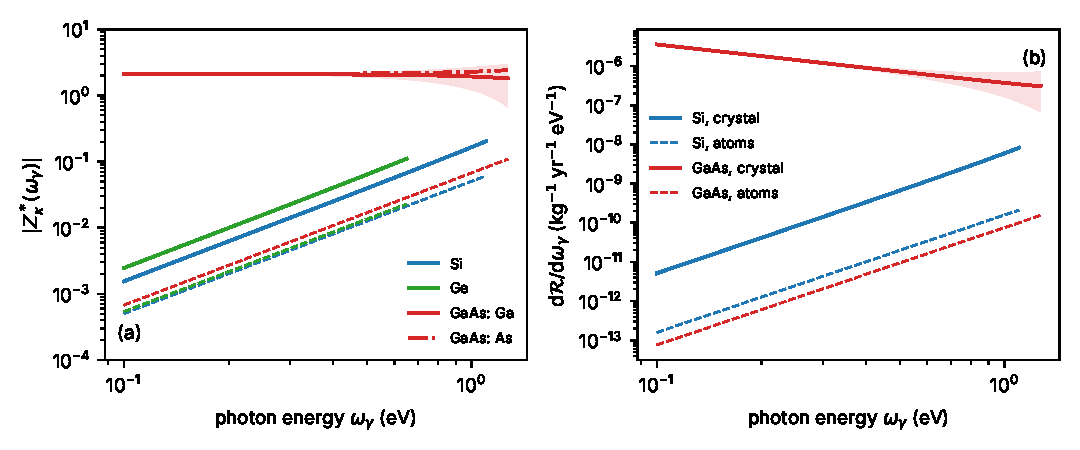
\includegraphics[width=\linewidth]{figures/ch12/fig12_5.pdf}
  \caption{Nuclear-recoil bremsstrahlung in silicon, germanium and GaAs below their absorption edges. (a) The dynamical Born charge $|Z^*_\kappa(\omega_\gamma)|$ against the photon energy (solid; dash-dotted for the arsenic site), from the sum rule \cref{eq:12.6-sum} with measured refractive indices: silicon at \SI{300}{K}~\cite{franta2017temperature} (0.1--\SI{1.1}{eV}), germanium at \SI{293}{K}~\cite{li1980refractive} (0.1--\SI{0.65}{eV}) and GaAs at \SI{295}{K}~\cite{skauli2003improved,polyanskiy2024refractiveindex} (0.1--\SI{1.27}{eV}, the range of the dispersion formula; its phonon term removed from the electronic $\varepsilon$). GaAs: $Z^* = 2.11$ at zero frequency and the dispersion of the sum split equally between the sites; shaded, the range allowed by the bound $|Z^*_\kappa(\omega) - Z^*_\kappa(0)| \le 0.9\,(\omega/\SI{1}{eV})^2$. Dashed: the free atoms, \cref{eq:12.6-atom} with the static polarizabilities 37.3 (Si), 40 (Ge) and 50 (Ga) atomic units~\cite{schwerdtfeger2019table}. (b) Rate per unit photon energy for $\mchi = \SI{100}{MeV}$, a heavy mediator coupled to nucleon number, $\sigma_p = 10^{-38}\,\mathrm{cm}^2$, the halo of \cref{sec:1.2}, \cref{eq:12.6-brems} with a free recoil. Solid: crystals; dashed: the same nuclei with the free-atom charges and $n_r = 1$; shaded: the GaAs band of panel (a).}
  \label{fig:12-brems}
\end{figure}

\Cref{fig:12-brems} shows the result. In GaAs the photons per kick are almost flat in $\ln\omega_\gamma$, as for a bare charge; half of them lie below \SI{0.36}{eV}. In silicon and germanium the spectrum climbs as $\omega_\gamma^3$ up to the absorption edge. The absolute numbers are small. A recoil of \SI{100}{eV} emits $4.0\times10^{-13}$ photons between 0.1 and \SI{1.1}{eV} in silicon and $1.7\times10^{-10}$ between 0.1 and \SI{1.27}{eV} in GaAs, against the Migdal probability of $6.1\times10^{-3}$ in silicon at the same recoil. At \SI{100}{MeV} the GaAs rate in panel (b) integrates to $9\times10^{-7}$ events per kilogram-year, and the silicon rate to $2\times10^{-9}$, while the Migdal rate of silicon with the same coupling is 30 (\cref{sec:12.3-rate}). The photons of GaAs lie below the gap, where the Migdal effect is closed, but they come with a Migdal signal above the gap that, judged by silicon, is larger by more than seven orders of magnitude. Bremsstrahlung in these crystals is therefore a check of the theory, not a search channel. At photon energies of hundreds of eV and above, where Kouvaris and Pradler found the reach of their xenon search, $\varepsilon \to 1$, the crystal emits as its atoms, and \cref{eq:12.6-sum} returns the bare charges as the electrons fall behind.

\begin{workedexample}{The GaAs enhancement over the atomic rate}\label{we:12-gaas}
How much more does a GaAs crystal radiate than a gas of the same atoms? We work at $\omega_\gamma = \SI{1}{eV}$ and then over the transparent band.

\emph{The dynamical Born charges.} The cell volume is $\Omega = a^3/4 = \SI{44.80}{\angstrom^3}$ with the static-lattice constant $a = \SI{5.638}{\angstrom}$ of \cref{tab:E-functionals}, the cell of the computed phonons and Born charge of \cref{sec:5.5}, and $\Omega m_e/e^2 = \SI{3.249e-2}{eV^{-2}}$. The dispersion formula of Skauli and collaborators~\cite{skauli2003improved}, as tabulated in Ref.~\cite{polyanskiy2024refractiveindex}, gives $n_r = 3.4185$ at \SI{1}{eV}, and without its phonon term the electronic dielectric function $\varepsilon = 11.688$. By \cref{eq:12.6-sum} at $\omega = \SI{1}{eV}$ the sum of the charges is $-(3.249\times10^{-2})(10.688) = -0.347$. Split equally, $Z^*_{\mathrm{Ga}}(\SI{1}{eV}) = 2.11 - 0.174 = 1.936$ and $Z^*_{\mathrm{As}}(\SI{1}{eV}) = -2.11 - 0.174 = -2.284$, so that the sum of their squares is 8.965. For any other split the sum of squares is $2(2.11 + b)^2 + 2(0.174)^2$, with $b$ half the difference between the two dispersions; the band of \cref{fig:12-brems} carries the values of $b$ that the bound allows.

\emph{The free atoms.} With $\alpha_{\mathrm{pol}} = 50$ and 30 atomic units~\cite{schwerdtfeger2019table}, that is $4\pi\times50\,a_0^3 = \SI{93.1}{\angstrom^3}$ and \SI{55.9}{\angstrom^3} in Heaviside--Lorentz units, \cref{eq:12.6-atom} gives $Z^*_{\mathrm{at}} = -0.0675$ for gallium and $-0.0405$ for arsenic at \SI{1}{eV}, and the sum of squares is $6.20\times10^{-3}$.

\emph{Per photon.} The two nuclei have nearly the same nucleon number per mass and nearly the same $q^2/M_\kappa^2$ at a given recoil, so the ratio of \cref{eq:12.6-brems} to its atomic form is the ratio of $n_r\sum_\kappa Z^{*2}_\kappa$ to $\sum_\kappa Z^{*2}_{\mathrm{at},\kappa}$: $3.4185\times8.965/6.20\times10^{-3} = 4.94\times10^3$ at \SI{1}{eV}. The crystal emits five thousand times more. Of that, $n_r$ contributes 3.4 and the Born charge the rest.

\emph{Over the band.} The ratio grows toward small $\omega_\gamma$ as $\omega_\gamma^{-4}$, since the atomic charges fall as $\omega_\gamma^2$ and the crystal charges do not. Integrated with the weight $1/\omega_\gamma$ of \cref{eq:12.6-brems} from 0.1 to \SI{1.27}{eV}, $\int n_r\sum_\kappa Z^{*2}_\kappa\,\dd\omega_\gamma/\omega_\gamma = 75.4$ and $\int\sum_\kappa Z^{*2}_{\mathrm{at},\kappa}\,\dd\omega_\gamma/\omega_\gamma = 4.03\times10^{-3}$, a ratio of $1.87\times10^4$. The full rate at $\mchi = \SI{100}{MeV}$ gives $1.88\times10^4$, the same to the precision shown, because the kinematics hardly depends on photon energies so far below the kinetic energy of the dark matter.

\emph{Per recoil.} A gallium nucleus with $E_R = \SI{100}{eV}$ has $v_N^2 = 2E_R/M = 3.08\times10^{-9}$, and with $2\alpha/3\pi = 1.549\times10^{-3}$ it emits $1.7\times10^{-10}$ photons in the band. The enhancement over the atom is large, four orders of magnitude, but it multiplies a small number. Its uncertainty is the band of \cref{fig:12-brems}: the rate at \SI{100}{MeV} lies between \SI{-19}{\percent} and \SI{+25}{\percent} of its central value.
\end{workedexample}

\subsection{Migdal-type absorption of a scalar}\label{sec:12.6-absorption}

A scalar of mass \SI{1}{keV} from the halo, absorbed in silicon, deposits \SI{1}{keV} with a momentum of only $k = m_\phi v \approx \SI{1}{eV}$. If it couples to nucleons, the nucleus takes that momentum, and its recoil energy, $k^2/2M_\kappa$, is \SI{e-11}{eV}. The energy must go somewhere else, and it goes to the electrons. Dzuba, Flambaum and Samsonov computed this for atoms~\cite{dzuba2024migdal}. In the language of \cref{sec:12.2} it is a Migdal effect at the momentum $k$ instead of $q$. The exact center-of-mass separation \cref{eq:12.2-cm} turns the kick $\ee^{\ii\vect{k}\cdot\vect{X}}$ into a kick of the whole atom and the boost $\exp(-\ii\vect{k}_e\cdot\sum_e\vect{\rho}_e)$ of the electrons, with $\vect{k}_e = m_e\vect{k}/m_A$. At the dipole order of \cref{eq:12.2-dipole} the amplitude to excite the electrons to $\Psi_f$ is $-\ii k_e\langle\Psi_f|D_{\hat k}|\Psi_0\rangle$. What differs from scattering is the energy. The field supplies $\omega = m_\phi$, and the whole of it goes to the electrons, $\omega_e = m_\phi$, while the lattice receives nothing to the precision of interest.

\emph{The coupling.} A scalar coupled to protons and neutrons, $\mathcal{L} \supset \phi\,(g_{\phi pp}\,\bar pp + g_{\phi nn}\,\bar nn)$, couples to each nucleus coherently, as in \cref{eq:8.1-nuclear}, with the nuclear form factor equal to one at these momenta. The interaction is $H_\phi = -\phi\sum_\kappa c_\kappa n_\kappa(\vect{p}_\phi)$, the nuclear density row of \cref{sec:8.1-absorption} with
\begin{equation*}
  c_\kappa = Z_\kappa\,g_{\phi pp} + (A_\kappa - Z_\kappa)\,g_{\phi nn} , \qquad g^\phi_{n_\kappa} = -c_\kappa ,
\end{equation*}
the per-species weight $c_\kappa$ of \cref{sec:11.3}, which here carries the couplings themselves rather than their ratio to a reference coupling. For equal couplings, $c_\kappa = A_\kappa g_{\phi nn}$.

\emph{The acceleration form.} For an atom the center-of-mass separation is exact; in a crystal there is no atom to separate, and we need another route to the same amplitude. The equations of motion give it. Whatever the interactions, the potential energy $V$ of the crystal depends on the positions alone, so $[H,\vect{X}_I] = -\ii\vect{P}_I/M_\kappa$ and $[H,\vect{P}_I] = \ii\nabla_{\vect{X}_I}V$, and the double commutator is $[H,[H,\vect{X}_I]] = \nabla_{\vect{X}_I}V/M_\kappa$. Between eigenstates with $\omega_{fi} = E_f - E_i \neq 0$ this reads $\omega_{fi}^2\langle f|\vect{X}_I|i\rangle = \langle f|\nabla_{\vect{X}_I}V|i\rangle/M_\kappa$. Expanding the kick to first order in $\vect{k}$,
\begin{equation}
  \Bigl\langle f\Big|\sum_Ic_\kappa\ee^{\ii\vect{k}\cdot\vect{X}_I}\Big|i\Bigr\rangle = \frac{\ii}{\omega_{fi}^2}\sum_I\frac{c_\kappa}{M_\kappa}\,\vect{k}\cdot\langle f|\nabla_{\vect{X}_I}V|i\rangle + O(k^2) ,
  \label{eq:12.6-accel}
\end{equation}
the acceleration form of the amplitude. It is exact, at every order of the Born--Oppenheimer expansion. Its matrix element is minus the total force on nucleus $I$, from the electrons and the other nuclei, between the initial and final states. Between electronic states this is the derivative coupling of \cref{eq:5.1-dcoup}, and \cref{eq:12.6-accel} is the boost amplitude \cref{eq:8.6-boost} with $q$ replaced by $k$ and the excitation energy by $\omega_{fi}$. In scattering the boost is the first term of an expansion in the velocity of the nucleus. Here the momentum is so small that only the dipole term matters, and the equations of motion give it exactly.

\emph{Couplings proportional to mass.} Let $c_\kappa = \tilde cM_\kappa$ for every species, with one constant $\tilde c$. The potential depends only on differences of positions, so the gradients with respect to all particles sum to zero, $\sum_I\nabla_{\vect{X}_I}V = -\sum_j\nabla_{\vect{r}_j}V$, the sum over electrons: the total force on the nuclei is minus the total force on the electrons. The same double commutator for the electrons, with $m_e$ in place of $M_\kappa$, turns the right-hand side of \cref{eq:12.6-accel} into a dipole matrix element of the electrons, and
\begin{equation}
  \Bigl\langle f\Big|\tilde c\sum_IM_\kappa\ee^{\ii\vect{k}\cdot\vect{X}_I}\Big|i\Bigr\rangle = -\tilde c\,m_e\,\langle f|n_e(\vect{k})|i\rangle\,\bigl[1 + O(kr)\bigr] ,
  \label{eq:12.6-mass}
\end{equation}
with $r$ the size of the states involved. The physical reading is the equivalence principle. A field that couples to the mass of every particle cannot, at zero momentum, distinguish them: it pushes the center of mass and nothing else, and its matrix elements between different states start at order $k^2$. A coupling to the mass of the nuclei is the coupling to the total mass minus that to the electrons, and only the second term excites the crystal. It is the electronic counterpart of the cancellation by which a coupling proportional to mass excites no optical phonon (\cref{eq:11.8-Gamma}).

The scalar therefore acts on the electrons as a density coupling of strength $\tilde cm_e$. The absorption formula \cref{eq:8.2-abs} with $S_{ee} = (2k^2/e^2)L$, \cref{eq:4.4-SL}, the electron-density form that holds above the phonon band, gives the rate.
\begin{keyresult}[Migdal-type absorption in a crystal]
For a scalar whose couplings to the nuclei are proportional to their masses, $c_\kappa = \tilde cM_\kappa$, absorbed with momentum $\vect{p}_\phi$ and energy $\omega_\phi \simeq m_\phi$ above the phonon band,
\begin{equation}
  \varGamma_{\mathrm{abs}} = \frac{\tilde c^2m_e^2\,p_\phi^2}{e^2\,m_\phi}\,L(\vect{p}_\phi \to 0, m_\phi) , \qquad
  \mathcal{R} = \frac{\rho_\chi}{\rho_T}\,\frac{\tilde c^2m_e^2\langle v^2\rangle}{e^2}\,L(m_\phi) ,
  \label{eq:12.6-absrate}
\end{equation}
with $L = \Imag[-1/\varepsilon]$ the loss function at zero momentum and $\langle v^2\rangle$ the mean squared speed of the halo in the laboratory.
\end{keyresult}
\noindent For the halo of \cref{sec:1.2}, $\langle v^2\rangle^{1/2} = \SI{379}{km.s^{-1}}$. The spectrum is that of dark-photon absorption, whose rate is $(\rho_\chi/\rho_T)\zeta^2L(m_\phi)$ (\cref{sec:10.7}), with $\zeta^2$ replaced by $\tilde c^2m_e^2\langle v^2\rangle/e^2$. Everything \cref{sec:10.7} found about screening carries over: the scalar is absorbed with the loss function, not with the absorptive part $\varepsilon_2$, suppressed near the absorption peaks of silicon, where $|\varepsilon|^2$ is large, and enhanced at the plasmon. In silicon and germanium, with one species, every coupling to nucleons is proportional to the mass up to the isotopes, so \cref{eq:12.6-absrate} is the whole rate.

The atomic result is the dilute limit. For a gas, $|\varepsilon| \to 1$ and $L \to \varepsilon_2$, and the photoabsorption cross-section $\sigma_\gamma$ of one atom fixes $\omega\varepsilon_2 = \nd_{\mathrm{at}}\sigma_\gamma$, with $\nd_{\mathrm{at}}$ the density of atoms. Then $\varGamma_{\mathrm{abs}} = \nd_{\mathrm{at}}v\,\sigma_\phi$ with $\sigma_\phi = \tilde c^2m_e^2(p_\phi/m_\phi)\sigma_\gamma/e^2$, which for $\tilde c = g_{\phi nn}/m_p$ is the relation of Dzuba, Flambaum and Samsonov between scalar absorption and photoionization~\cite[Eqs.~(14), (17)]{dzuba2024migdal}. They cautioned that rates in solids could differ from the atomic estimate, and \cref{eq:12.6-absrate} says by how much. Applied to a crystal with the measured photoabsorption, which in a medium is $\nd_{\mathrm{at}}\sigma_\gamma = \omega\varepsilon_2/n_r$, the atomic formula uses $\varepsilon_2/n_r$ where the crystal has $\varepsilon_2/|\varepsilon|^2$. The ratio, $n_r/|\varepsilon|^2$, is the medium factor. Far above the absorption edges, $\varepsilon \simeq 1 - \omega_p^2/\omega^2$ with $\omega_p$ the plasma frequency of the electrons bound below $\omega$, so that $n_r \simeq 1 - \omega_p^2/2\omega^2$ and $|\varepsilon|^2 \simeq 1 - 2\omega_p^2/\omega^2$, and
\begin{equation}
  \frac{n_r}{|\varepsilon|^2} = 1 + \frac32\,\frac{\omega_p^2}{\omega^2} + O\Bigl(\frac{\omega_p^4}{\omega^4},\ \varepsilon_2^2\Bigr) .
  \label{eq:12.6-medium}
\end{equation}
For silicon at \SI{1}{keV}, with the twelve electrons per atom bound by less than \SI{1}{keV} and $\omega_p = \SI{28.8}{eV}$, this is $1 + 1.2\times10^{-3}$. Near the plasmon and the absorption peaks it is far from one.

\begin{limitbox}[Migdal-type absorption of a scalar][lim:12.6a]
$\sigma_\phi = g_{\phi nn}^2(m_e^2/m_p^2)(p_\phi/m_\phi)\,\sigma_\gamma/4\pi\alpha$ per atom, with $\sigma_\gamma$ the photoionization cross-section at $\omega = m_\phi$~\cite[Eqs.~(14), (17)]{dzuba2024migdal}.
\par\smallskip
{\centering
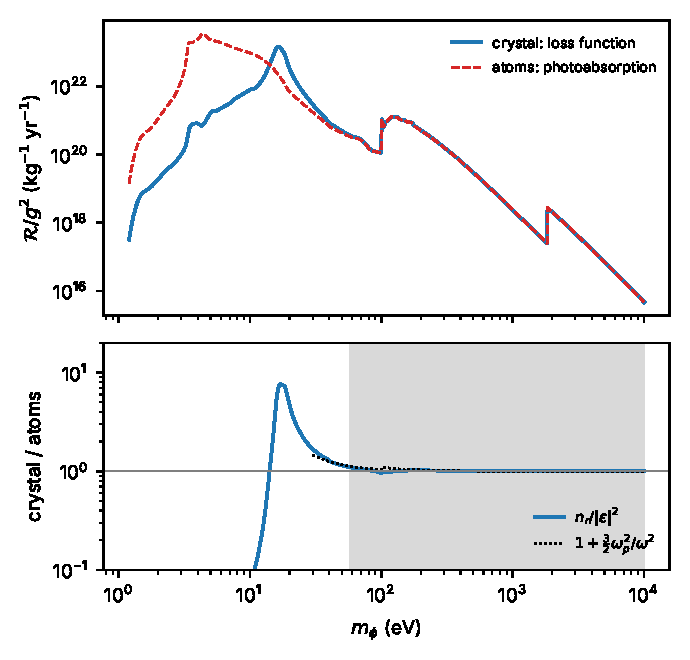
\includegraphics[width=0.92\linewidth]{figures/ch12/limit12_6a.pdf}
\captionof{figure}{Absorption of a scalar coupled equally to protons and neutrons ($c_\kappa = gA_\kappa$) in silicon against its mass $m_\phi$. Top: rate per unit mass divided by $g^2$, from the loss function, \cref{eq:12.6-absrate} (solid), and from the atomic formula with the measured photoabsorption of the crystal, $\nd_{\mathrm{at}}\sigma_\gamma = m_\phi\varepsilon_2/n_r$ (dashed); halo of \cref{sec:1.2}. Bottom: their ratio $n_r/|\varepsilon|^2$, with the expansion \cref{eq:12.6-medium} (dotted, $\omega_p$ from the electrons bound below $m_\phi$, binding energies of the $L$ and $K$ shells as in \cref{sec:10.6}). Dielectric function of silicon at \SI{300}{K}~\cite{franta2017temperature} below \SI{40}{eV} and from the atomic scattering factors~\cite{henke1993xray} above, as in \cref{sec:10.7}. Gray band: $m_\phi \ge \SI{57}{eV}$, where the atomic formula is within \SI{10}{\percent}.}\label{fig:12-limit-6a}
\par}
\smallskip
Below about \SI{60}{eV} the atomic formula misses the screening of the crystal, and is too high by about 400 near the absorption peak at \SI{4.2}{eV} and too low by 7.7 near the plasmon, at \SI{17}{eV}.
\end{limitbox}

\noindent On the truncation label \cref{lim:12.6a} sits at dipole order, $n_D = 2$ in the rate, with no Born--Oppenheimer truncation, since \cref{eq:12.6-accel,eq:12.6-mass} are exact; $\mathcal{X}$ is the measured loss function, and the lattice plays no role at these energies. Its next corrections are the multipoles of order $kr$, which at \SI{10}{keV} and a $1s$ radius of $a_0/Z$ are below $10^{-3}$, and, outside the shaded band, the full loss function in place of the atomic formula.

\emph{Couplings not proportional to mass.} If $c_\kappa/M_\kappa$ differs between species, write it as $\tilde c + \delta\tilde c_\kappa$, with $\tilde c$ a mean. The mean part is \cref{eq:12.6-absrate}. The remainder keeps the forces in \cref{eq:12.6-accel}, $\ii\omega^{-2}\sum_I\delta\tilde c_\kappa\,\vect{k}\cdot\langle f|\nabla_{\vect{X}_I}V|i\rangle$, and these no longer sum to anything simple. For transitions of the electrons the force on a nucleus is the density component of \cref{eq:12.1-force}, the vertex of the Migdal entry. The sum over the sites of one species, weighted by $\ee^{\ii\vect{k}\cdot\vect{X}_I}$, then forces the momentum given to the electrons to be $\vect{k} + \vect{G}$. The remainder is therefore a sum over reciprocal-lattice vectors weighted by the basis structure factor of $\delta\tilde c_\kappa Z_\kappa$, and it samples the off-diagonal elements $S^{ee}_{\vect{0}\vect{G}}$ and $S^{ee}_{\vect{G}\vect{G}'}$ of the electronic response at vanishing reduced momentum (\cref{eq:E.18-X}). These are nonadiabatic matrix elements in the sense of \cref{sec:12.1}: the response of the electrons to the force of one sublattice, which no optical measurement provides. For the core shells, which belong to one nucleus, the atomic dipole formula with $\delta\tilde c_\kappa$ in place of $\tilde c$ applies shell by shell. For the valence electrons \cref{app:E.18} specifies the calculation, with $S^{ee}_{\vect{G}\vect{G}'}$ to $|\vect{G}| = 6(2\pi/a)$ and the test that the (200) channel of the diamond structure vanishes for equal $\delta\tilde c_\kappa$. How large the remainder is depends on the coupling. For nucleon number in GaAs the two species differ in $A_\kappa/M_\kappa$ by $2.6\times10^{-5}$ per u (\cref{we:8-nucleon}), and the remainder is negligible. For a coupling to protons alone, $Z_\kappa/M_\kappa$ is 0.4446 per u for gallium and 0.4405 for arsenic, and the isotopes of natural silicon differ by up to \SI{7}{\percent}; the isotopic part is a random remainder, incoherent between sites, like the isotope scattering of \cref{sec:11.6}.

A scalar may also couple to electrons. Its amplitude adds $\tilde cm_e$ to the density coefficient $g^\phi_{n_e} = -g_{\phi ee}$ of \cref{eq:8.1-scalar}, and the kinetic row of the electron coupling, which dominates its absorption (\cref{sec:10.7}), interferes with the density row through their cross response. The nucleon coupling adds no new row.

\subsection{Nuisance table of the Migdal sector}\label{sec:12.6-table}

\Cref{tab:12-nuisances} collects the truncations and inputs of the chapter, each with its size and the section that treats it, in the classes of \cref{sec:8.8}.

\begin{table}[tbp]
  \caption{Nuisances of the Migdal sector. Type in the classes of \cref{sec:8.8}: normalization, tilt (in $\omega_e$, in $q$ or in the dark-matter mass), threshold and lattice spectrum (the share of a Migdal event that goes to phonons, at fixed electronic energy transfer). Basis of the size: ``computed'' (next order computed), ``model'' (next order computed in a model), ``est.''\ (parametric estimate), ``bound'' (only an inequality is known), ``named'' (no size). Sizes are for silicon unless another crystal is named. The last column gives the section where the item is treated.}
  \label{tab:12-nuisances}
  \centering\footnotesize\setlength{\tabcolsep}{3pt}
  \begin{tabular}{@{}>{\raggedright\arraybackslash}p{0.27\linewidth}>{\raggedright\arraybackslash}p{0.12\linewidth}>{\raggedright\arraybackslash}p{0.36\linewidth}>{\raggedright\arraybackslash}p{0.09\linewidth}>{\raggedright\arraybackslash}p{0.10\linewidth}@{}}
    \toprule
    Truncation or input & Type & Size & Basis & Section \\
    \midrule
    Local fields on the diagonal of $\varepsilon^{-1}$ (scalar $\varepsilon$ against $\varepsilon^{-1}_{\vect{G}\vect{G}}$) & normali\-zation; tilt in $\omega_e$ & factor 1.35 on the total, concentrated at $p \gtrsim q_{\mathrm{BZ}}$ (\cref{lim:12.3a}) & computed & \cref{sec:12.3} \\
    Off-diagonal elements $\vect{G} \neq \vect{G}'$ of $\varepsilon^{-1}$ & normali\-zation & raises the rate: full over diagonal 1.38 at $8^3$ points $\vect{k}$ and $|\vect{G}|^2 \le 19\,(2\pi/a)^2$, about 1.2 extrapolated, in an empirical-pseudopotential random-phase model of Si that carries about 2/3 of the diagonal local-field effect; still falling with $\vect{G}$, so the lower end is not a bound; flat in $\mchi$; the full local-field calculation is open; incoherent, zone-averaged form, not applicable at $q \ll q_{\mathrm{BZ}}$ & model & \cref{sec:12.1,sec:12.3} \\
    Loss-function table ($\omega_e \le \SI{89}{eV}$, $p \le \SI{22.5}{keV}$) & normali\-zation & $P_{\mathrm{Mig}}$: $\le\SI{1.6}{\percent}$ above \SI{89}{eV}; $p > \SI{10}{keV}$ holds \SI{2.3}{\percent}; drag mass: missing part $\le\SI{24}{\percent}$ & bound & \cref{sec:12.3,sec:12.5} \\
    Ion charge $Z_{\mathrm{ion}}(p)$ against a point ion & normali\-zation & $P_{\mathrm{Mig}}$ $\times1.57$; drag mass $18.6$ against $11.8\,m_e$ & model & \cref{sec:12.3,sec:12.5} \\
    Valence on-site drag mass & normali\-zation of the added lattice rate & Si $18.6\,m_e$ (12 to $24\,m_e$), Ge $39.5\,m_e$ (11.5 to $52\,m_e$); trace value $14\,m_e$ is not the on-site element & bound & \cref{sec:12.5} \\
    Per-mass form of the rate & tilt in $\mchi$ & within \SI{10}{\percent} above \SI{66}{MeV} & computed & \cref{sec:12.3} \\
    Frame of the transition density (lattice at $\vect{q} - \vect{p}$ or $\vect{q}$; Herzberg--Teller) & lattice spectrum & phonon-emitting fraction $\times2.4$ at \SI{5}{keV}; $+\SI{12}{\percent}$ in the displaced-oscillator model & model & \cref{sec:12.1,sec:12.4} \\
    Incoherent lattice factor below the zone & lattice spectrum & zero-phonon line within \SI{8}{\percent} of the Bragg sum; multiphonon terms uncertified below \SI{6.6}{keV} & computed; named & \cref{sec:12.4} \\
    Coherent zero-phonon response at $q < 2q_{\mathrm{BZ}}$ (cross-site terms of the lattice factor) & normali\-zation; tilt in $\omega_e$ & limit $q \ll q_{\mathrm{BZ}}$ (\cref{eq:8.3-boostward}): $1/14.9$ of the diagonal form, median $\omega_e$ \SI{17.4}{eV} against \SI{4.5}{eV}; within \SI{15}{\percent} only for $q \le \SI{0.75}{keV}$ (model), which carries $\le\SI{0.2}{\percent}$ of the rate at every mass; \SI{0.75}{keV} to $2q_{\mathrm{BZ}}$ unsized, nearly all of the rate up to \SI{1}{MeV}, \SI{33}{\percent} at 2 and \SI{7}{\percent} at \SI{3}{MeV} & computed (limit); model; unsized & \cref{sec:12.4} \\
    Exact energy denominators (recoil of $\vect{p}$, binding, Doppler; \cref{eq:12.3-bracket,eq:12.4-corr}) & tilt in $q$ & near the gap $-2.1\times10^{-3}$, $+2.8\times10^{-3}$ and at most $5.1\times10^{-4}$ below the impulse onset; free recoil: probability within \SI{10}{\percent} to $E_R \approx \SI{160}{eV}$, factor 1.6 at \SI{500}{eV}, rate within \SI{10}{\percent} to \SI{1}{GeV} & computed & \cref{sec:12.3,sec:12.4} \\
    Germanium lattice inputs (Debye-scaled) & lattice spectrum & $\langle\omega^{-1}\rangle^{-1} \approx \SI{17.6}{meV}$ from $\Theta_{\mathrm{D}} = \SI{373}{K}$; regime boundaries near 41 and \SI{113}{keV}; no first-principles phonon spectrum & est. & \cref{sec:12.4} \\
    Dipole order of the atomic boost (cores) & tilt in $q$ & within \SI{10}{\percent} to $\xi_D = 0.188$ (Si), 0.127 (Ge) & computed & \cref{sec:12.2} \\
    Bound final states of the atom & normali\-zation & lower bound only & bound & \cref{sec:12.2} \\
    Wannier picture of the boost & normali\-zation & absolute bound 1.6, 0.54, 0.25 at 20, 50, \SI{100}{eV}; non-rigid ratio open & bound & \cref{sec:12.3} \\
    Relativistic contact density (third moment) & normali\-zation of the check & $+\SI{8}{\percent}$ (Si), $+\SI{42}{\percent}$ (Ge); non-logarithmic Dirac remainder and $p_{1/2}$ contact density uncontrolled, each of relative order $(Z\alpha)^2$ (\SI{5}{\percent} in Ge) & computed; est. & \cref{sec:12.5} \\
    Site difference of $Z^*_\kappa(\omega)$, GaAs bremsstrahlung & normali\-zation & $-19$ to $+\SI{25}{\percent}$ at \SI{100}{MeV} & bound & \cref{sec:12.6} \\
    Atomic formula for Migdal-type absorption & tilt in $m_\phi$ & within \SI{10}{\percent} above \SI{57}{eV}; about $400\times$ high at \SI{4.2}{eV} & computed & \cref{sec:12.6} \\
    Couplings not proportional to mass & normali\-zation & Umklapp remainder (\cref{eq:E.18-X}) & named & \cref{sec:12.6} \\
    \bottomrule
  \end{tabular}
\end{table}

For the silicon Migdal probability above a few MeV the table has one large computed row, the local fields on the diagonal, and one large row sized only in a model, the off-diagonal part, which acts in the opposite direction. The table truncation, by contrast, costs a few percent, and the ion charge is fixed by the frozen core. The per-mass form is not an uncertainty of a correct calculation but the error of a simpler one, and its size says where the simpler one may be used. The counting of Migdal and lattice events depends on the on-site drag mass, which is known only within a factor of two. And the frame of the transition density changes how a Migdal event shares its energy between electrons and lattice without changing how many events there are, which matters to a detector that reads both charge and phonons.

\subsection{Open problems}\label{sec:12.6-open}

The dynamical Born charges of a polar crystal are fixed by \cref{eq:12.6-sum} only in their sum; the difference between the sites needs the frequency-dependent calculation of \cref{app:E.17}, and until it is done the GaAs bremsstrahlung rate carries the band of \cref{fig:12-brems}. And the absorption of a scalar whose couplings are not proportional to the masses needs the off-diagonal response $S^{ee}_{\vect{G}\vect{G}'}$ at vanishing reduced momentum, which \cref{app:E.18} specifies. The open items of the earlier sections are rows of \cref{tab:12-nuisances}. Above all of them stands a measurement. No crystal Migdal signal has yet been observed. A tagged-recoil measurement, in which the energy and direction of each nuclear recoil are fixed independently, for instance by the kinematics of a neutron scattered at a known angle, and the electrons it releases are counted, would test the whole chain at once in silicon at the recoil energies of \cref{sec:12.5}.

\section*{Summary}

A kicked nucleus leaves energy in two places, the lattice and the electrons, and the joint response resolves the two (\cref{sec:12.1}). It is the response of \cref{sec:8.7} sorted by the electronic energy transfer $\omega_e$ and the lattice energy $\omega_l$; its marginal is the ordinary response, and the sectors of \cref{sec:8.6} fall on the two axes and the quadrant between them. At the leading nonadiabatic order its Migdal entry is the response of the electrons to the field of a suddenly moving nucleus: a boost $\vect{q}\cdot\vect{p}/M_\kappa\omega_e^2$, the bare vertex of the nucleus, the density response of the clamped electrons and the lattice response at the momentum the nucleus keeps. The four published Migdal formulas are truncations of that entry. Its first moment is fixed by the drag mass, and the estimate $P_{\mathrm{Mig}} \approx (E_R/\langle\omega_e\rangle)(\delta M_\kappa/M_\kappa)$ follows. Added to a lattice rate, a Migdal rate requires the lattice response with the weight $1 - P_{\mathrm{Mig}}$ and the dragged mass, and a measured nuclear-recoil yield already contains the Migdal ionization. In a metal the sudden expansion fails at small $\omega_e$.

The isolated atom is the truncation in which the boost can be done to all orders (\cref{sec:12.2}). The center of mass separates exactly, and the electrons receive the momentum $m_e\vect{q}/m_A$, with $m_A$ the mass of the whole atom. At dipole order the ionization probability at a recoil energy of \SI{1}{keV} is $2.09\times10^{-3}$ for silicon and $1.63\times10^{-3}$ or $1.73\times10^{-3}$ for germanium in two independent calculations, and the dipole form holds within \SI{10}{\percent} up to $\xi_D = 0.188$ and 0.127. Bound final states without ionization add to it, and the oscillator strengths give only a lower bound on their share. In a crystal the atomic form is the right one for the core shells, not for the valence.

At large momentum transfer the crystal Migdal probability is a weighted moment of the loss function, with the coefficient $4\alpha$ fixed by the $f$-sum rule and the valence ionization factor $Z_{\mathrm{ion}}(p)$ in the vertex (\cref{sec:12.3}). In silicon it is $6.1\times10^{-5}$ per eV of recoil energy, 29 times the atomic value. A scalar dielectric function overestimates it by about \SI{35}{\percent}, an error concentrated at $p \gtrsim q_{\mathrm{BZ}}$; the off-diagonal elements of the dielectric matrix raise it in a model by a factor of about 1.4 as computed and 1.2 extrapolated, the lower end not a bound, and their full calculation is open. The soft limit has no correction in $p/q$ and holds at low mass; it fails only when the nucleus moves fast during the transition, above about \SI{160}{eV} of recoil. The factorized rate per unit mass holds within \SI{10}{\percent} above \SI{66}{MeV}. The Wannier picture of the boost is exact for flat bands and bounded only in absolute terms for the valence band of silicon.

Below the impulse onset the lattice factor of the Migdal entry is the multiphonon response at the momentum the nucleus keeps (\cref{sec:12.4}). The electronic spectrum does not depend on it, since the lattice factor has unit weight. What it decides is how a Migdal event shares its energy: at \SI{10}{keV} in silicon \SI{92}{\percent} of the events leave the lattice in its ground state, and most events stay zero-phonon until the zero-phonon weight of the kick itself falls to one half, at \SI{33.2}{keV}. The phonon-mediated form is the same process with the bound-nucleus propagator, exact in the phonon energies at first order in $\vect{p}$; for silicon and germanium its correction is a few parts in a thousand at the gap, and it matters only where gaps approach phonon energies.

The moments of the Migdal spectrum are inverse moments of the force that the electrons exert on one nucleus (\cref{sec:12.5}). The first is the on-site drag mass, which differs from the trace value of $14\,m_e$ for silicon that a uniform translation fixes; the loss function gives $18.6\,m_e$ for the valence electrons alone, uncertain by a factor of two. Two moments bound the probability from both sides. The cross first moment fixes the Migdal interference of a mixed coupling, and the third moment is the electron density at the nucleus, which relativity raises by \SI{8}{\percent} in silicon and \SI{42}{\percent} in germanium.

A recoiling nucleus also radiates, and an absorbed scalar coupled to nucleons gives its energy to the electrons through the same boost (\cref{sec:12.6}). The crystal emits with the dynamical Born charge, which in silicon and germanium follows exactly from the measured dielectric function and suppresses the emission as the fourth power of the photon energy. Silicon still emits 33 to 38 times more than its atoms, and GaAs, with its static Born charge, $1.87\times10^4$ times more over its transparent band. The rates are seven orders below the Migdal rate, so bremsstrahlung is a check, not a channel. A scalar whose couplings to the nuclei are proportional to their masses is absorbed with the loss function, by the equivalence principle, and the atomic formula holds in silicon only above \SI{57}{eV}. The chapter's nuisances are collected in \cref{tab:12-nuisances}. Throughout, the electronic final states were reached by kicking a nucleus; \cref{chap:13} turns to the other mixed sector, the electrons kicked directly while a phonon carries the missing momentum.

\printbibliography[heading=subbibliography]
